%% Abraham Tishelman-Charny's PhD Thesis 
%% 14 June 2022

\documentclass[thesis]{neu}
\input{packages}
% If you are using the alpha bibliography style, keep these next three lines in your preamble, so that the references are left-aligned; or, you can comment it out and see what happens
\makeatletter
\renewcommand{\@biblabel}[1]{[#1]\hfill}
\makeatother

% \title{
% \fontsize{20}{0}  \selectfont Search for Higgs boson pair production in the \texorpdfstring{WW$\gamma\gamma$}{WWyy} final state at the CMS experiment with Run 2 LHC Data
% }

\title{
Search for Higgs boson pair production in the \texorpdfstring{WW$\gamma\gamma$}{WWyy} final state \\ \newline at the CMS experiment with Run 2 LHC Data
}

% Author name
\author{Abraham Tishelman-Charny}

% Department
\department{Department of Physics} 

% Default style for front pages
\frontpagestyle{1} % 7 is preferred by Rackham, but should be set individually for each front page

% Acknowledgments (the input [7] determines the style -- 7 is Rackham's preferred style)
\acknowledgments{ 
    I first would like to thank my advisor, Toyoko Orimoto. I am sincerely grateful to have had an advisor who has been on my side every step of the way during the course of my PhD, and who clearly prioritized my well-being above all else. Toyoko always enthusiastically encouraged me to follow my heart when it came to choosing research projects and activities, which led to me enjoying my research. I would not have had such a meaningful and fruitful PhD experience if it were not for her. 

I would also like to thank the HH to WW$\gamma\gamma$ analysis team: Mingshui Chen, Peiran Li, Petr Mandrik, Badder Marzocchi, Fabio Monti, Ram Krishna Sharma, Sergei Slabospitskii, Junquan Tao, Joshuha Thomas-Wilsker, Chu Wang, and Jin Wang. One of the many fortunate circumstances which made my PhD experience special was the opportunity to lead a physics analysis working group. I am grateful to have had that opportunity, through which I learned from everybody in the group. 

During my PhD, I was also very fortunate to be part of the wonderful CMS ECAL community. While I am grateful for all of the many people who I have learned from in this group, I would like to express special thanks to Giacomo Cucciati, David Petyt, and Davide Valsecchi. Giacomo was always incredibly kind and willing to thoroughly answer my countless questions about ECAL DAQ, and was a great partner in crime at ECAL Run Coordination. The experience I have gained working with David has been invaluable and an important part of my PhD. David was also willing to answer my endless questions, in this case about ECAL TPG, and always took the time to share his insightful perspective and feedback as the projects we worked on developed over time. Finally, whether it was through Italian lessons or ECAL trigger discussions, Davide and I always had \textit{fun} with what we discussed. This was an absolutely essential aspect of our work. Keeping things fun kept us interested in collaborating over our multi-year projects. 

I also want to thank Tanvi, Chad and Andrew for keeping me company while we were under lockdown during the pandemic. All of the meaningful conversations, support, silly jokes, and laughter kept me sane.  

Finally, I want to thank my parents for encouraging me to pursue a PhD in the first place, and for believing in me more than I believed in myself. 
}

\abstract{
    \input{Sections/abstract}
}

\hidepreface

% Committee
\committee{ %
Professor Toyoko Orimoto, Chair \\
Professor Emanuela Barberis \\
Professor James Halverson \\
Professor Darien Wood
}

% Chair must be entered separately for formatting reasons.
\chair{Professor Toyoko Orimoto}

%%-- Begin Document
\begin{document}
% \maketitle
% \doublespacing
% \tableofcontents
% \singlespacing % if you want single spacing after showing the table of contents
\newpage 

\input{common-definitions} 

% Define variables for only rendering certain portions of the document, in order to save time when editing a section.
\newcounter{RenderPreAnalysisSections}
\setcounter{RenderPreAnalysisSections}{1}

\newcounter{RenderAnalysisSection}
\setcounter{RenderAnalysisSection}{1}

\newcounter{RenderAppendices}
\setcounter{RenderAppendices}{1}

% Build the desired chapters 

\ifthenelse{\value{RenderPreAnalysisSections}=1}
{

    \chapter{Introduction} \label{ch:introduction}
    Through the study of particle physics, human beings are able to probe the fundamental building blocks of the very universe they inhabit. This field is rich in expertise. Firstly, particle physicists seeking to answer fundamental questions about the universe determine the experimental setups, namely the types of particle accelerators and detectors, that are required in order to attempt to answer these questions. Incredible efforts are then required of engineers and technicians to build these accelerators and detectors. Multi-year long data-taking periods then commence, warranting undying dedication from a multitude of accelerator and detector operations teams. The unprecedented amounts of data recorded by these particle detectors, and their associated simulations, then require state of the art computational tools and resources to be processed and analyzed in a reasonable time frame. Finally, novel statistical interpretations must then be invoked in order to infer results from the recorded data, in an attempt to answer the questions with which physicists began. This monumental effort requires expertise from scientists around the world, where CERN (Organisation Europ\'eenne pour la Recherche Nucl\'eaire) is one of the main sites where these collaborators come together. 

In 2012, the experimental discovery of the Higgs boson by the CMS (Compact Muon Solenoid) and ATLAS experiments at the CERN LHC (Large Hadron Collider) \cite{Aad:2012tfa,Chatrchyan:2012ufa,Chatrchyan:2013lba} marked a historic achievement for humanity. Physicists had finally experimentally verified the existence of the Higgs boson, a particle first theorized in the 1960s, and one that is central to the current framework of particle physics: The Standard Model (SM).

The SM is a quantum field theory describing the fundamental forces of nature and its constituent particles. It accounts for the electromagnetic, weak, and strong forces and includes particles classified as quarks, leptons, and bosons. The SM is consistent with the vast majority of experimental observations in particle physics, and continues to be widely used to this day when interpreting data. Additionally, it is often used as a basis from which extensions are made to new theories. In the SM, observable particles arise as excitations of their corresponding quantum fields. The Higgs field adds a potential energy term to the SM Lagrangian, and due to its shape and the requirement of a vacuum energy value, its mathematically described symmetry is spontaneously broken. This process is known as electroweak symmetry breaking, and is a crucial mechanism described by the SM as it explains the origin of mass for massive particles which interact with the Higgs field.

In the post Higgs-discovery era, physicists are aiming to further understand and characterize the Higgs boson, and by extension the electroweak symmetry breaking mechanism. A fundamental test of the SM is to measure the coupling strengths of the Higgs boson to massive SM particles, where many couplings have now been measured with precisions down to around 10\% with respect to their SM predicted values. A coupling of particular interest which has not yet been precisely measured is the Higgs self-coupling. This coupling has a direct effect on the shape of the Higgs potential, and its magnitude is explicitly predicted by the SM. Based on this predicted value and the current measurements of the top quark mass and Higgs boson mass, it is predicted that the Higgs vacuum energy currently sits at a metastable minimum. This would mean there is a non-zero probability that the minimum of the Higgs potential can tunnel to a lower minimum, which would change the laws of physics as we know them. An experimental measurement of the Higgs self-coupling could have profound implications on physicists' understanding of the universe: It may confirm the predictions of the SM, or it may refute the SM entirely and prompt physicists to make sense of this in a way that is in agreement with all previous observations. 

Through the study of Higgs pair production, the production of two Higgs bosons in a single process, the Higgs self-coupling is directly accessible. Additionally, through the use of an Effective Field Theory (EFT) framework, a wide model-independent search for physics beyond the standard model (BSM) through searches of Higgs pair production can be performed. Due to destructive interference between its two leading order (LO) processes, non-resonant Higgs pair production has a low production cross section, meaning that the combination of many di-Higgs final states will be necessary in order to maximize the chances for observation, and obtain as precise a measurement as possible of the Higgs self-coupling. In order to search for this relatively small signal and include a new search channel, a search for Higgs pair production by the CMS experiment in the WW$\gamma\gamma$ channel was performed. This channel benefits from the sensitive H$\rightarrow\gamma\gamma$ process which provides a narrow, distinguishable signature. The H$\rightarrow$WW leg of the decay contributes a relatively large branching ratio among Higgs boson decay processes of about 22\%, increasing the expected yields of the di-Higgs process. Because the W boson can decay both leptonically and hadronically, the H$\rightarrow$WW and by extension the HH$\rightarrow$WW$\gamma\gamma$ process has three possible final states: The Fully-Hadronic, Semi-Leptonic, and Fully-Leptonic final states, corresponding to 0, 1, and 2 leptonically decaying W-bosons respectively.

During Run 2 of the LHC (2016-18), about 138 fb$^{-1}$ of data was recorded by the CMS detector from proton-proton collisions at a center-of-mass energy of $\sqrt{s}=13$ TeV. Using this dataset, the first search for Higgs pair production in the WW$\gamma\gamma$ final state by the CMS experiment was performed. The CMS ECAL (Electromagnetic Calorimeter) was vital for this analysis, as it is the sole sub-detector of CMS that can directly detect photons which leave a trace of the sensitive H$\rightarrow\gamma\gamma$ signature in all three final states of this di-Higgs channel. It is additionally crucial for the detection of electrons, present in two of the three WW$\gamma\gamma$ final states. 

In order to potentially improve the sensitivity of this analysis and similar analyses using the CMS dataset to be collected during Run 3 of the LHC beginning in 2022, existing CMS ECAL features have been optimized and new features have been investigated. During the commissioning period of the CMS ECAL for Run 3, the performance of the CMS ECAL operations teams will be crucial for the detector's successful operation and its commissioning of these features.

Additionally, it is important to estimate the expected sensitivity of this analysis and similar analyses using data to be collected by the upgraded CMS detector during the running period of the future High Luminosity LHC, in order to gauge the prospects of these future physics analyses. This is done through projection studies, the first of which in the WW$\gamma\gamma$ and $\tau\tau\gamma\gamma$ di-Higgs final states has been performed by the CMS collaboration.

This thesis is organized as follows: Chapter \ref{chapter:TheoreticalBackground} will describe the theoretical background which comprises our current understanding of particle physics, and inherently motivates experimental analyses. Chapter \ref{chapter:Experimental_Setup} will describe the experimental setup: The Large Hadron Collider and the CMS detector. Chapter \ref{chapter:HHWWyy} makes up the ``Past" portion of this thesis, and will describe the first search by the CMS collaboration for Higgs pair production in the two W-boson and two-photon final state. Chapter \ref{chapter:ECAL_Run3} makes up the ``Present" portion of this thesis, and will describe the ongoing efforts to optimize the CMS Electromagnetic Calorimeter for Run 3, a crucial subdetector for detecting photon and electron signatures of the HH$\rightarrow$WW$\gamma\gamma$ process. This chapter will also include a description of the roles of the various CMS ECAL operations teams. Chapter \ref{chapter:Phase_II_HH} makes up the ``Future" portion of this thesis, and will describe the first sensitivity projection of the search for Higgs pair production in the WW$\gamma\gamma$ and $\tau\tau\gamma\gamma$ final states at the future High Luminosity LHC with the upgraded CMS detector. Finally, Chapter \ref{chapter:summary} will summarize the full content of the thesis, and highlight the importance of making the most of the data taken in the past while simultaneously optimizing the quality of the data taken during the present, and investigating the potential prospects for physics analysis using data to be taken in the future. 
    
    \chapter{Theoretical background} \label{chapter:TheoreticalBackground}
    The history of particle physics encompasses a slew of discoveries of fundamental particles and force mediators that describe the matter and interactions of the universe. While much has been theorized and experimentally verified, the story of particle physics is far from over. As we progress, theoretical and experimental results will continue to influence other with the goal of understanding the nature of the universe. In this chapter, the current theoretical foundation of particle physics will be described in order to motivate the experimental setup and physics analyses later described in this thesis.

This chapter is structured as follows: The most successful theoretical model of particle physics to date, the standard model, will be described in Section \ref{sec:SM}. In Section \ref{sec:Higgs}, the Higgs boson and its corresponding electroweak symmetry breaking mechanism will be described. Finally, Section \ref{sec:Higgs_Pair_Production} will describe the process of Higgs pair production.

\section{The Standard Model} \label{sec:SM}

The standard model (SM) is a quantum field theory which defines a set of quantum fields, whose excitations correspond to observable particles, and describes how they interact. The SM is considered one of the most successful and widely encompassing physical theories to date, as it is consistent with most of the phenomena observed in particle and nuclear physics experiment, and therefore forms a bedrock of understanding of the nature of the universe. The SM defines a quantum field for each type of particle, where the particles include force mediating gauge bosons, a scalar boson, and fermions making up massive material. 

The difference between these two classes of particles is as follows: Bosons obey Bose-Einstein statistics, meaning many of them in a given system can simultaneously exist in the same quantum state, while fermions obey Fermi-Dirac statistics, under which no two fermions within a system can exist in the same quantum state. The particles described by the standard model are depicted in Fig \ref{fig:SM_Diagram}.  

%%-- Standard model diagram 
\begin{figure}[H]
    \centering
    \includegraphics[width=\textwidth]{Images/Theory/Standard_Model_of_Elementary_Particles.pdf}
    \caption{Particles described by the Standard Model}
    \label{fig:SM_Diagram}
\end{figure}

An important feature of the SM lagrangian is its invariance under the product group shown in Equation \ref{eq:ProductGroup}.

\begin{equation} \label{eq:ProductGroup}
    SU(3)_{C}\times SU(2)_{W}\times U(1)_{Y}
\end{equation}

The invariance of the SM lagrangian under these gauge groups corresponds to the conservation of color charge, weak isospin, and hypercharge. In addition, these gauge groups correspond to three fundamental forces: The electromagnetic force mediated by the photon (U(1)), the weak force mediated by the $W^{\pm}$ and Z bosons (SU(2)), and the strong force mediated by the gluon (SU(3)). A known fourth fundamental force of nature, the gravitational force, is not described by the standard model. The absence of the gravitational force in the standard model is a sign that while the SM explains the majority of observations, it is an incomplete description of the fundamental particles and interactions of the universe. 

\subsection{Particles}

The SM predicts the existence of particles, which manifest in observation as excitations of their corresponding quantum fields. The particles are classified as fermions described in Section \ref{sec:fermions}, and bosons described in Section \ref{sec:bosons}.

\subsubsection{Fermions} \label{sec:fermions}

Fermions are defined as particles which obey Fermi-Dirac statistics, meaning that no two fermions in a quantum system can occupy the same quantum state. At a macroscopic scale, this can be qualitatively thought of as the impossibility for two pieces of matter to go through each other. At a microscopic scale, one implication of Fermi-Dirac statistics is that as an atom gains more electrons, they must occupy ``shells'' at higher energy states, as lower energy states may already be occupied by existing electrons. 

The two types of fermions are quarks and leptons, each of which has three generations, increasing in mass with each generation. The quarks are composed of up and down (1st generation), charm and strange (2nd generation), and top and bottom quarks (3rd generation). When describing particle masses, the base unit used is the electronvolt (eV), where 1 eV corresponds to the amount of kinetic energy gained by an electron when accelerated from rest across one volt of electric potential in a vacuum. The six SM quarks have a large mass range spanning a few MeV up to 173 GeV (current mass measurement of the top quark), and account for the quantum numbers of hadrons. A common instance of quarks is the composition of the most common hadrons we see around us: Protons (neutrons) have three valence quarks: two up (down) quarks and one down (up) quark.

% https://en.wikipedia.org/wiki/Color_confinement

In the SM, quarks are predicted to be confined, meaning they cannot exist freely and must always be in a bound state with other particles. This means when quarks are produced in experiment, such as from particle collisions, these quarks immediately form pairs with quarks from the QCD vacuum. This process continues with subsequent quarks, leading to the detection of a jet of hadronic activity rather than a single quark. This phenomenon is called hadronization, and is shown in Figure \ref{fig:Quark_Hadronization}. This phenomenon is constantly seen at hadron colliders, and is a fundamental handle for detecting quarks and gluons.

\begin{figure}[H]
    \centering
    \includegraphics[width=\textwidth]{Images/Theory/Quark_confinement.png}
    \caption{Diagram of quark hadronization}
    \label{fig:Quark_Hadronization}
\end{figure}

The three generations of leptons are the electron, muon, and tau, each with a corresponding flavour of neutrino. Electrons are present in atoms, as they exist in quantum states surrounding the atomic nucleus comprised of neutrons and protons. 

While electrons, muons, and taus have mass, in the SM there is no mechanism by which neutrinos gain mass. However, experimental measurements of neutrino oscillations have observed non-zero differences between the squared masses of different neutrino flavors, implying that neutrinos have mass. This is further evidence that the SM is incomplete.  

All leptons also have an associated anti particle, which posses the same traits as its corresponding particle but with a negated electric charge. 

\subsubsection{Bosons} \label{sec:bosons}

Bosons are defined as particles which obey Bose-Einstein statistics. The SM predicts five bosons, namely the gluon, photon, Z boson, W boson and Higgs boson. 

Gluons are responsible for mediating the strong force, the mechanism which keeps protons in a bound state by binding their valence and sea quarks. The energy stored in this binding of quarks via gluons accounts for most of the mass of the proton. 

The photon is a massless boson which mediates the electromagnetic force between charged particles. It is also the particle corresponding what we see as light: Electromagnetic radiation, which at certain frequencies is visible to the human eye. 

% https://cds.cern.ch/record/2103277/files/9789814644150_0006.pdf?subformat=pdfa&version=1

The W and Z bosons mediate the weak force, and were experimentally discovered by the UA1 and UA2 experiments at CERN in 1983.

The quantum field corresponding to the Higgs boson plays the special role of providing the mechanism by which massive fermions and bosons obtain their mass. 

\subsection{Forces}

While predicting the existence of fermions and bosons, the SM also predicts three types of interactions between these particles: The strong, weak, and electromagnetic interactions. 

\subsubsection{The strong interaction}

The strong force is mediated by the gluon, and is the force by which gluons and quarks interact. This type of interaction is called Quantum Chromodynamics (QCD), and corresponds to the SU(3) gauge symmetry in the SM, for which color charge is the conserved quantity. 

This force is crucial to our qualitative conception of matter, as it is responsible for the binding of quarks into protons and neutrons, as well as the binding of protons and neutrons into stable molecules. 

\subsubsection{The weak interaction}

The weak force is a fundamental force mediated by the W$^{\pm}$ and Z bosons, and corresponds to the SU(2) gauge symmetry of the SM, whose conserved quantity is weak isospin. 

A fundamental concept in particle and nuclear physics is that of decay: Unstable particles tend to decay towards a more favorable energy state, in which they are transformed into subsequent ``daughter'' particles, and the weak force is the mechanism by which radioactive decays occur. A common decay known as beta decay, the process by which a neutron decays into a proton, does so via the decay of one of its valence quarks to the opposite signed quark. A Feynman diagram illustrating this is shown in Figure \ref{fig:BetaDecay_FD}. 

\begin{figure}[H]
    \centering
    \includegraphics[width=0.65\textwidth]{Images/Theory/Beta_Decay_FD.png}
    \caption{Feynman diagram of $\beta$ decay.}
    \label{fig:BetaDecay_FD}
\end{figure}

In this interaction, the down-flavoured valence quark of a neutron (d) spontaneously decays into an up quark via the emission of a W boson. This W boson then subsequently decays into an electron and an anti-electron neutrino, leaving a traceable signature. This is known as the lepton decay mode of the W boson, and is one signature through which physicists can search for the W boson in particle collisions.

\subsubsection{The electromagnetic interaction}

The electromagnetic interaction is mediated by the photon, a spin 1 gauge boson. The conserved quantity in the SM through this interaction is hypercharge, corresponding to the U(1) gauge symmetry in the SM, illustrated in Equation \ref{eq:U1_Symmetry}. 

\begin{equation} \label{eq:U1_Symmetry}
    \phi\rightarrow\phi^{\prime}=e^{i\alpha}\phi
\end{equation}

Where $\phi$ represents a scalar field, and $\alpha$ represents a constant. Under this transformation the SM lagrangian is invariant.

The photon interacts with all electromagnetically charged particles, which includes quarks, massive leptons, and the W boson. An example interaction, that of the repulsion of two electrons via the electromagnetic force, is shown in the form of a Feynman diagram in Figure \ref{fig:EM_FD}.

\begin{figure}[H]
    \centering
    \includegraphics[width=0.65\textwidth]{Images/Theory/EM_FD.png}
    \caption{Feynman diagram of the electromagnetic interaction between two electrons.}
    \label{fig:EM_FD}
\end{figure}

\section{The higgs boson and electroweak symmetry breaking} \label{sec:Higgs}

While the electromagnetic and weak forces can be defined individually, and act separately at low energy scales, at the electroweak energy scale of about 246 GeV, they are unified into a single force called the electroweak force. This energy scale is convenient for describing the potential energy term from the Higgs boson, and the subsequent spontaneous breaking of its symmetry.

The Higgs potential term of the SM lagrangian looks as shown in Equation \ref{eqm-1}.

\begin{eqnarray}
  V(\Phi) = - \frac{\mu^2}{2}\left|\Phi \right|^2
  +\frac{\lambda}{4} \left|\Phi \right|^4
  \label{eqm-1}
\end{eqnarray}

The shape of the higgs potential is shown in Figure \ref{fig:HiggsPotential}, in a two dimensional phase space made up of the real and imaginary parts of the field $\Phi$. 

\begin{figure}[H]
    \centering
    \includegraphics[width=0.65\textwidth]{Images/Theory/Higgs_Potential_Shape.png}
    \caption{Shape of the Higgs potential}
    \label{fig:HiggsPotential}
\end{figure}

A minimum energy value, or vacuum expectation value (VEV), must be taken by the higgs potential. Due to the shape of the higgs potential, an infinite number of points in the two dimensional phase space made up by the real and imaginary parts of the field $\Phi$ lie on a circle which all take on the same value of the Higgs potential. This means that a choice must be made as to which point is taken for the VEV, which leads to a spontaneous breaking of this symmetry. 

After electroweak symmetry breaking, additional terms are added to the lagrangian including mass terms for the known massive particles, and terms which determine the shape of the Higgs potential, shown in Equation \ref{eq:HiggsPotentialShape}. 

\begin{eqnarray}
  V &=& \frac{m_H^2}{2}H^2 + \lambda_3 v H^3 + \frac{\lambda_4}{4} H^4,
\quad
 \lambda_3 = \lambda_4 = \lambda_{HHH} = \frac{m_H^2}{2v^2} \label{eq:HiggsPotentialShape}
\end{eqnarray}

Thus, the shape of the higgs potential depends on the coupling strength values of a Higgs to two Higgs (the tri-linear coupling $H^{3}$), and of two Higgs to two Higgs (the quartic Higgs coupling $H^{4}$). The values of these couplings are predicted by the SM in terms of the Higgs boson mass and VEV, and based on experimental measurements the higgs self-coupling is predicted to be 0.13 by the SM.  

% After electroweak symmetry breaking, the higgs potential gains additional terms leading to the relations shown in Equation \ref{eq:Higgs_Relations}.

% \begin{eqnarray} \label{eq:Higgs_Relations}
%   \lambda = \frac{m_H^2}{2 v^2}, \;\;  \mu^2 = \frac{m_H^2}{2},
%   \;\; m_H^2 = \frac{\partial^2 V}{\partial \phi^2}
%   \label{eqm-2}
% \end{eqnarray}

% Additionally, 

Based on its predicated shape and the current measurements of the top quark mass and Higgs boson mass, the type of stability in which the Higgs VEV is predicted to sit is shown in Figure \ref{fig:HH_Stability_Plot}. 

\begin{figure}[H]
    \centering
    \includegraphics[width=0.65\textwidth]{Images/Theory/HH_stability_Plot.png}
    \caption{Higgs VEV stability as a function of top quark mass and Higs mass}
    \label{fig:HH_Stability_Plot}
\end{figure}

Based on current measurements of the top quark mass and Higgs boson mass, the Higgs VEV is predicted to sit at a meta-stable minimum, as depicted in Figure \ref{fig:PossibilityToTunnel}. 

\begin{figure}[H]
    \centering
    \includegraphics[width=0.65\textwidth]{Images/Theory/HH_potential_Stability.png}
    \caption{Depiction of a metastable Higgs VEV.}
    \label{fig:PossibilityToTunnel}
\end{figure}

This allows for a non-zero probability of the Higgs minimum to shift to a lower, global minimum value, through the process of quantum tunnelling. A shift of the minimum of this sort would completely change the laws of physics as we understand them. 

As this is the prediction made by the SM based on the current top quark and Higgs boson mass measurements, it is crucial to be able to compare this to experiment. This implies that an experimental measurement of the shape of the Higgs potential, accessible via its tri-linear and quartic couplings, would provide a fundamental test of the SM. 
\section{Higgs pair production} \label{sec:Higgs_Pair_Production}

A process through which the Higgs self-coupling can be directly accessed is Higgs pair production, the production of two Higgs bosons in a single process. The access of this coupling can allow for a measurement of its value, meaning that physics analyses of Higgs pair production can allow physicsts to provide experimental input into the shape of the Higgs potential. This comparison would be fundamental, and could have profound implications: This measurement may agree with the SM, or it may disagree and prompt physicists to consider how to reconcile the SM with their current observations. 

The two Feynman diagrams at leading order (LO) which have the largest impact on the production likelihood of Higgs pair production in the gluon-gluon fusion production mode are shown in Figure \ref{fig:HH_GF_LO_FD}.

\begin{figure}[H]% 
    \setcounter{subfigure}{0} % reset subcaption counter to 0 (a) 
    \centering
    \subfloat[Triangle diagram]{\includegraphics[width=.45\linewidth]{Images/Theory/fey_HH_Triangle.pdf}}%
    \qquad
    \subfloat[Box diagram]{\includegraphics[width=.45\linewidth]{Images/Theory/fey_HH_Box.pdf}}%
    \caption{Leading order Higgs pair production Feynman diagrams in the gluon-gluon fusion production channel.}%
    \label{fig:HH_GF_LO_FD}
\end{figure}  

These diagrams are referred to as the ``triangle'' and ``box'' diagrams, where the triangle diagram is sensitive to both the Higgs self-coupling and top yukawa coupling (the coupling of the Higgs boson to two top quarks), while the box diagram is sensitive only to the top yukawa coupling. These diagrams destructively interfere in the computation of the process' matrix element, leading to a low production cross section. The contributions and interference of these two diagrams as a function of di-Higgs invariant mass for a center-of-mass energy of proton-proton collisions equal to $\sqrt{s} = 14 TeV$ is shown in Figure \ref{fig:LOXS_Contributions}. 

\begin{figure}[H]
    \centering
    \includegraphics[width=0.85\textwidth]{Images/Theory/LO_contributions_ggF.pdf}
    \caption{Contribution to HH production cross section as a function of di-Higgs system invariant mass, for the triangle and box diagrams and their interference term.}
    \label{fig:LOXS_Contributions}
\end{figure}

Taking the higher order Feynman diagrams into account, including at next to leading order (NLO) and next-to-next-to leading order (NNLO), a more precise value of the di-Higgs production cross section is computed as a function of center of mass energy for different production modes, and is shown in Figure \ref{fig:ProductionModeXSs}. 

\begin{figure}[H]
    \centering
    \includegraphics[width=0.85\textwidth]{Images/Theory/cxn_HH.pdf}
    \caption{Higgs pair production cross sections for different production modes, as a function of center of mass energy.}
    \label{fig:ProductionModeXSs}
\end{figure}

For proton-proton collisions at center-of-mass energies between 13-100 TeV, the dominant production mode of Higgs pair production is gluon-gluon fusion. For most of this energy spectrum, the next most sensitive production mode is Vector Boson fusion, roughly a factor of 20 less likely. Theoretical productions of Higgs pair production cross section, and physics processes in general, are extremely important for motivating the types of particle colliders and detectors to be built in the future. This allows the matching of a desired physics program with colliders and experiments expected to be capable of producing and detecting these expected physics signatures, in order to answer physicists' questions. 
    
    \chapter{Experimental Setup: The LHC and the CMS Detector} \label{chapter:Experimental_Setup}
    From the theoretical background described in the previous chapter, we know what type of physics we expect to see given an initial set of conditions. In order to test the consistency of this theory and search for its expected signatures in order to answer fundamental questions, we require an experimental setup designed to produce and study these physical interactions. 

This chapter is divided into two sections: Section \ref{sec:LHC} will describe the Large Hadron Collider, and Section \ref{sec:CMS} will describe the Compact Muon Solenoid detector. 

\section{The Large Hadron Collider} \label{sec:LHC}

The Large Hadron Collider is a particle accelerator located about 100 meters underground, straddling the border of France and Switzerland. It is the largest machine ever built, and an aerial view is shown in Fig \ref{fig:LHC_BirdsEye}, including the positions of the major experiments it delivers collisions to: The ALICE, ATLAS, CMS, and LHCb detectors. Its construction took place from 1998 to 2008, with the intention of building a machine which can produce proton-proton collisions at a center of mass energy not yet achieved, where part of its physics program was to experimentally discover the Higgs boson, and enhance the ability to test a variety of beyond the standard model (BSM) theories. 

\begin{figure}[H]
    \centering
    \includegraphics[width=\textwidth]{Images/LHC/LHCCollage_withExperiments.jpeg}
    \caption{The geographical location of the Large Hadron Collider (yellow solid), relative to the French-Swiss border (white dashed) and LHC experiments (white labels)}
    \label{fig:LHC_BirdsEye}
\end{figure}

The LHC is the final acceleration stage in a complex of linear and circular accelerators, all of which are depicted in Figure \ref{fig:CERN_Acc_Complex}. 

\begin{figure}[H]
    \centering
    \includegraphics[width=\textwidth]{Images/LHC/CERN_Accelerator_Complex.png}
    \caption{CERN accelerator complex}
    \label{fig:CERN_Acc_Complex}
\end{figure}

% https://www.lhc-closer.es/taking_a_closer_look_at_lhc/0.proton_source
% https://home.cern/science/accelerators/proton-synchrotron-booster
% https://home.cern/science/accelerators/proton-synchrotron
% https://home.cern/science/accelerators

Proton-proton collisions are a useful basis for performing a variety of particle physics analyses, as with a high enough initial energy, all of the SM fermions and bosons can be produced. As the mass of the proton is small compared to that of other SM particles such as the W and Z bosons (about 1/90th) or the Higgs boson (about 1/125th the mass), particle accelerators are used in order to increase the energy of the protons such that this energy can be converted into these more massive particles. Also as seen in the theoretical background chapter, higher center-of-mass energies can lead to higher likelihoods of producing rare processes, such as Higgs pair production. 

In Figure \ref{fig:LHC_Long_Term_Schedule}, the long term schedule of the LHC is shown. It should be noted that this schedule is always subject to change, as unforeseen circumstances may come up during this long time period.

% At the end of LHC Run 3, the LHC will enter Long Shutdown 3 (LS3), where the LHC will be upgraded to the High Luminosity LHC (HL-LHC). The LHC long term schedule, which is subject to change, is shown in Figure \ref{fig:LHC_Long_Term_Schedule}.

\begin{figure}[H]
    \centering
    \includegraphics[width=\textwidth]{Images/LHC/LHC_LongTermSchedule_MyVersion.png}
    \caption{LHC long term schedule}
    \label{fig:LHC_Long_Term_Schedule}
\end{figure}

\subsection{Run 2}

Run 2 of the LHC took place from 2015-2018 as shown in Figure \ref{fig:LHC_Long_Term_Schedule}, where very little data was delivered to the experiments in 2015, and therefore the vast majority of Run 2 analyses include data collected from 2016-2018. 

In order to prepare proton-proton collisions with a high center of mass energy and instantaneous luminosity, during LHC Run 2 the CERN accelerator complex began with a source of H$_{2}$, a hydrogen gas. This H$_{2}$ gas was injected into a cavity in the presence of an electric field in order to strip it of its electrons, yielding a pure proton source. These protons were then sent to LINAC 2 (Linear Accelerator 2) to perform an initial acceleration of protons to an energy of 50 MeV. The proton beam then enters the Proton Synchrotron Booster, where they are further accelerated to 1.4 GeV for injection into the Proton Synchrotron, where the beam is further accelerated to 26 GeV. The penultimate stop in the proton beams' acceleration journey is the Super Proton Synchrotron (SPS). In SPS, proton are accelerated up to 450 GeV each and are then injected into the LHC. It is in the LHC where the proton beams, during Run 2, were accelerated up to 6.5 TeV each corresponding to a center of mass energy of 13 TeV, then a world record. 

Each stage of acceleration is performed thanks to a variety of superconducting magnets and radio-frequency cavities, with additional magnets used to focus the beams.

During LHC Run 2, the LHC delivered about 156 fb$^{-1}$ of proton-proton collisions to the CMS and ATLAS experiments, with a average number of simultaneous collision interactions, known as pile-up, around 36. 

% https://twiki.cern.ch/twiki/bin/view/AtlasPublic/LuminosityPublicResultsRun2

\subsection{Run 3}

Run 3 of the LHC is expected to last from 2022-2025, as shown in Figure \ref{fig:LHC_Long_Term_Schedule}. During LHC Run 3, the acceleration stages will generally be the same as during LHC Run 2, but with the replacement of LINAC 2 in favor of LINAC 4. 

On July 5th 2022, the LHC delivered its first ``stable beam" collisions at a new world record center-of-mass energy: 13.6 TeV, corresponding to beam energies of 6.8 TeV each, displayed on the LHC monitor shown in Figure \ref{fig:LHCMonitor_first13p6TeV}. 

\begin{figure}[H]
    \centering
    \includegraphics[width=\textwidth]{Images/LHC/First_13p6TeV_Collisions.png}
    \caption{LHC monitor during the first stable beams collisions at $\sqrt{s} = 13.6$ TeV}
    \label{fig:LHCMonitor_first13p6TeV}
\end{figure}

This marked the official start of LHC Run 3. The LHC will spend July 2022 increasing the number of proton bunches in the machine, and starting around the end of July 2022 and early August 2022, will have a full machine of proton bunches in order to provide high intensity collisions to the experiments so that large amounts of data can be recorded.

During LHC Run 3, it is expected that the average pileup will be around 55 simultaneous interactions per bunch crossing, and early estimates of total integrated luminosity are about double that delivered during Run 2. Due to this increase in pileup and total radiation dose to the detectors, it will be important to continue to optimize the LHC detectors during Run 3 to ensure quality data is taken. 

\subsection{The High-Luminosity LHC}

At the end of LHC Run 3, the LHC will enter Long Shutdown 3 (LS3), during which the LHC will be upgraded to the High Luminosity LHC (HL-LHC). The HL-LHC is then planned to deliver record amounts of collisions data to the experiments over Runs 4 and 5 between the years 2029-2038, as shown in Figure \ref{fig:LHC_Long_Term_Schedule}. 

The sensitivity and uncertainty of a plethora of physics analyses is driven by the yields, or number of events, of the analyzed dataset. Increasing the number of events of the available data to be used for analysis is one of the main motivations for upgrading the LHC, allowing for a higher integrated luminosity which will lead to more sensitive BSM searches, and more precise SM measurements. 

The HL-LHC expects to deliver an unprecedented 3000 fb$^{-1}$ to the main LHC experiments, which will make up about 90\% of the experiments' total datasets. A visualization of the integrated luminosity to be delivered by the LHC and HL-LHC over time, with a slightly shifted timeline, is shown in Figure \ref{fig:LHC_Int_Lumi}.

\begin{figure}[H]
    \centering
    \includegraphics[width=\textwidth]{Images/LHC/LHC-nom-lumi-proj-with-ions.png}
    \caption{LHC and HL-LHC expected integrated luminosity over time} % https://lhc-commissioning.web.cern.ch/schedule/images/LHC-nom-lumi-proj-with-ions.png
    \label{fig:LHC_Int_Lumi}
\end{figure}

While the upgraded HL-LHC will deliver extremely large datasets to the experiments, this will also lead to very challenging data-taking conditions: One aspect will be the increased pileup which will be produced during HL-LHC collisions, expected to increase from about 55 simultaneous interactions during Run 3 data-taking, to about 140 during HL-LHC. This means that while more interesting signal-like interactions may occur during this data-taking period, there will be many more less-interesting background interactions which will need to be separated from signal interactions. Additionally, during this period detectors will receive a very large amount of radiation which will degrade their sub-detectors. In order to deal with the increase in pileup and radiation, the LHC experiments plan to implement major upgrades so that they can collect high quality data during HL-LHC in order to extend their BSM reaches and SM measurement precisions. 
% All of the answers are here: https://twiki.cern.ch/twiki/bin/viewauth/CMS/Internal/PubDetector

\section{The CMS detector} \label{sec:CMS}

The Compact Muon Solenoid (CMS) is a general purpose particle detector located at one of the main interaction points of the LHC. CMS began operation at the start of the LHC in 2009, and collected data delivered by the LHC during LHC Runs 1 (2010-12) and 2 (2015-18). CMS has just recently completed its commissioning phase and started recording data as a part of LHC Run 3, which officially began in July 2022. CMS resides in an underground cavern (UXC), shown in Figure \ref{fig:CMS_image}.

\begin{figure}[H]
    \centering
    \includegraphics[width=\textwidth]{Images/CMS/CMS.jpg}
    \caption{The Compact Muon Solenoid}
    \label{fig:CMS_image}
\end{figure}

CMS is designed as a hermetic layered structure made of different technologies in order to detect different particles coming from proton-proton and heavy ion collisions delivered by the LHC. A slice of the CMS detector and its different technologies, and the different particles detected, is shown in Figure \ref{fig:CMS_PF}.

\begin{figure}[H]
    \centering
    \includegraphics[width=\textwidth]{Images/CMS/CMS_PF.png}
    \caption{CMS detector technologies and particles detected.}
    \label{fig:CMS_PF}
\end{figure}

% Generic CMS description below:

% The central feature of the CMS apparatus is a superconducting solenoid of 6\unit{m} internal diameter, providing a magnetic field of 3.8\unit{T}. 
% Within the solenoid volume are a silicon pixel and strip tracker, a lead tungstate crystal electromagnetic calorimeter (ECAL), and a brass and scintillator 
% hadron calorimeter (HCAL), each composed of a barrel and two endcap sections. Forward calorimeters extend the pseudorapidity coverage provided by the barrel 
% and endcap detectors. Muons are measured in gas-ionization detectors embedded in the steel flux-return yoke outside the solenoid. A more detailed description 
% of the CMS detector, together with a definition of the coordinate system used and the relevant kinematic variables, can be found in Ref.~\cite{CMS:2008xjf}.

% Events of interest are selected using a two-tiered trigger system. The first level (L1), composed of custom hardware processors, uses information from the 
% calorimeters and muon detectors to select events at a rate of around 100\unit{kHz} within a fixed latency of about 4\mus~\cite{CMS:2020cmk}. The second level, 
% known as the high-level trigger (HLT), consists of a farm of processors running a version of the full event reconstruction software optimized for fast processing, 
% and reduces the event rate to around 1\unit{kHz} before data storage~\cite{CMS:2016ngn}.

% In the barrel section of the ECAL, an energy resolution of about 1\% is achieved for unconverted or late-converting photons in the tens of GeV energy range. 
% The energy resolution of the remaining barrel photons is about 1.3\% up to $\abs{\eta} = 1$, changing to about 2.5\% at $\abs{\eta} = 1.4$. In the endcaps, 
% the energy resolution is about 2.5\% for unconverted or late-converting photons, and between 3 and 4\% for the other ones~\cite{CMS:2015myp}.

% The diphoton mass resolution, as measured in $H\rightarrow\gamma\gamma$ decays, is typically in the 1--2\% range, depending on the measurement of the photon 
% energies in the ECAL and the topology of the photons in the event~\cite{CMS:2020xrn}.

% The integrated luminosities for the 2016, 2017, and 2018 data-taking years have 1.2--2.5\% individual uncertainties~\cite{CMS-LUM-17-003,CMS-PAS-LUM-17-004,CMS-PAS-LUM-18-002}, 
% while the overall uncertainty for the 2016--2018 period is 1.6\%.

\subsection{Tracker}
The CMS tracker is the innermost layer of CMS, and is composed of silicon pixel and strip trackers. The main purpose of the tracker is to detect tracks left by electrically charged particles. These tracks are used to measure particle momentum, corresponding to the track's radius. Additionally, the tracker is used to identify the sign of the particle's charge, and is crucial for identifying the vertex of hard interactions from LHC collisions. The tracker is the most sensitive of the CMS sub-detectors, and is subject to the brunt of radiation produced by LHC collisions.  

\subsubsection{Pixel tracker} \label{sec:PIXEL}

The innermost layer of the CMS detector, and first layer of the CMS tracker, is the pixel tracker. This pixel tracker is composed of silicon sensors, of which there were initially about 65 million individual pixel readout channels in 2016. After the first full year of Run 2 data taking in 2016, the pixel detector was upgraded to the Phase-I pixel detector \cite{PhaseI_Pixel} in order to maintain performance following the upgrade of the LHC during the first Long Shutdown (LS1) from 2013-14, from which an instantaneous luminosity larger than the original pixel detector design was produced. The Phase-I pixel detector was installed during the 2016 Year End Technical Stop (YETS), which lasted from December 2016 to April 2017. After its installation, the Phase-I pixel detector, now containing about 124 million individual channels, was used during the 2017 and 2018 data-taking periods of Run 2.

The pixel tracker is composed of the Barrel (BPIX) and Forward (FPIX) pixel detectors, which result in a combined pseudorapidity region for particle detection of $|\eta| < 2.5$. A layout of the Phase-I pixel detector, and a comparison to the original design, is shown in Figure \ref{fig:Pixel_Tracker}. 

% \begin{figure}[H]
%     \centering % trim=left botm right top
%     \includegraphics[clip, trim=0cm 0cm 0cm 6cm , width=\textwidth]{Images/CMS/Tracker/Tracker_Phase_Compare.pdf}
%     \caption{The Phase-I CMS pixel detector (upper), compared to its original design (lower).}
%     \label{fig:Pixel_Tracker}
% \end{figure}

\begin{figure}[H]
    \centering % trim=left botm right top
    \includegraphics[width=\textwidth]{Images/CMS/Tracker/Tracker_Phase_Compare.pdf}
    \caption{The Phase-I CMS pixel detector (``Upgrade"), compared to its original design (``Current").}
    \label{fig:Pixel_Tracker}
\end{figure}

It can be seen that the main additions to the original CMS pixel detector are the addition of a layer in BPIX, and the addition of several disks in FPIX. Half of the BPIX system during production is shown in Figure \ref{fig:BPIX_Half}. In this image, the four half-circles concentric to the center of the image correspond to the four layers, L1-4. 

\begin{figure}[H]
    \centering
    \includegraphics[width=0.7\textwidth]{Images/CMS/Tracker/BPIX.png}
    \caption{Half of the Phase-I BPIX.}
    \label{fig:BPIX_Half}
\end{figure}

The Phase-I pixel detector was able to deliver its expected performance, as shown in Figure \ref{fig:PIX_HitEfficiency}. 

\begin{figure}[H]
    \centering
    \includegraphics[width=\textwidth]{Images/CMS/Tracker/Pixel_HitEfficiency.pdf}
    \caption{Pixel hit efficiency during 2018.}
    \label{fig:PIX_HitEfficiency}
\end{figure}

The hit efficiency is shown as a function of different instantaneous luminosities during the 2018 data-taking year of Run 2, where higher values correspond to a higher number of simultaneous interactions, and therefore harsher data-taking conditions. Hit efficiency is defined as the probability that a cluster of pixel hits corresponds to an extrapolated track. Layers 1-3 of BPIX, and the entire FPIX were able to maintain hit efficiencies around 99\% even for large instantaneous luminosity values of 2*$ 10^{34}$cm$^{-2}$s$^{-1}$. Additionally, the L1 hit efficiency, which suffers the most from the harsh data-taking conditions at it is closest to the interaction region, begins to drop around 1.4*$10^{34}$cm$^{-2}$s$^{-1}$ down to about 97.5\% at 2cm$10^{34}^{-2}$s$^{-1}$. However, this performance is greater than what would have been expected from the original pixel tracker which ran during 2016. 

This is an example of a detector upgrade which was unforeseen but deemed necessary to implement, in response to the data-taking conditions presented to CMS based on collisions delivered by the LHC.

\subsubsection{Strip tracker}

% https://pos.sissa.it/309/013/pdf
% https://twiki.cern.ch/twiki/bin/view/CMSPublic/DPGResultsTRK

The second layer of the CMS detector, and outer portion of the CMS tracker, is the strip tracker. A view of one quarter of the Phase I strip tracker used during Run 2 can be seen in Figure \ref{fig:Strip_Tracker}. 

\begin{figure}[H]
    \centering
    \includegraphics[width=0.7\textwidth]{Images/CMS/Tracker/upper-Schematic-view-of-the-CMS-tracker-detector-1-and-lower-closeup-view-of-the.png}    
    \caption{A view of half of the CMS strip detector in the r-z plane of CMS.}
    \label{fig:Strip_Tracker}
\end{figure}

The CMS strip tracker is composed of 15,148 silicon sensors which are spread over several partitions to cover different regions around the collision point: The Tracker Outer Barrel (TOB), Tracker Inner Barrel (TIB), Tracker Inner Disks (TID) with a plus and minus side, and Tracker Endcaps (TEC) which have modules on the plus and minus side. As shown in the diagram, the strip tracker surrounds the pixel tracker described in Section \ref{sec:PIXEL}. 

The strip tracker performs the same task as the pixel tracker, namely recording hits from electromagnetically charged particles in order to track their movement - a vital task for measuring particle $p_{T}$, identifying interaction vertices, and identifying jets from quark/gluon hadronization. The pixel and strip measurements are combined in order to obtain more accurate track measurements.  

During Run 2, the strip tracker maintained an excellent signal over noise ratio, and held a very stable percentage of problematic channels during Run 2, shown in Figure \ref{fig:Run2_StripTracker}.

\begin{figure}[H]% 
    \setcounter{subfigure}{0} % reset subcaption counter to 0 (a) 
    \centering
    \subfloat[2017 Signal over noise of TIB ]{\includegraphics[height=.25\textheight]{Images/CMS/Tracker/StripTracker_SON_TIB_SOverN_run296786_2017A.pdf}}%
    \qquad
    \subfloat[Run 2 problematic channel fraction ]{\includegraphics[height=.25\textheight]{Images/CMS/Tracker/run2_stripBadComponent_All.pdf}}%
    \caption{Run 2 strip tracker performance.} \label{fig:Run2_StripTracker}
\end{figure}  

In 2017, TIB had an excellent MPV (Most probable value) of 17.5 as a signal-to-noise ratio, indicating good signal detection in the strip tracker partition closest to the CMS interaction point. Additionally, over the course of Run 2 operations the percentage of bad components remain stable at about 4\% even after receiving the full Run 2 intergrated luminosity, highlighting the robustness of the detector. 

\subsection{Calorimeters}
The two calorimeters contained within the CMS detector are the Electromagnetic Calorimeter (ECAL), and the Hadronic Calorimeter (HCAL). A description of ECAL is provided in Section \ref{sec:ECAL}, and a description of HCAL is provided in Section \ref{sec:HCAL}. 

% \subsubsection{The Electromagnetic Calorimeter}\label{sec:ECAL}

% The CMS Electromagnetic Calorimeter is the second layer of the CMS detector, with respect to the interaction point of collisions produced by the LHC. In this Chapter, the CMS ECAL will first be introduced in Section \ref{sec:ECAL_Introduction}. In Section \ref{sec:ECAL_TPG}, the method of ECAL Trigger Primitive Generation as input to the CMS L1 trigger will be described. In Section \ref{sec:DW}, the development and commissioning of a new ECAL feature known as ``Double Weights" will be described, and in Section \ref{sec:ECAL_Operations} the various ECAL operations teams and their responsibilities will be described.  

\input{Sections/ECAL/sections/Introduction}
% \input{Sections/ECAL/sections/Trigger_primitive_generation}
% \input{Sections/ECAL/sections/Operations}

\subsubsection{The Hadronic Calorimeter}\label{sec:HCAL}

% arxiv 1910.00079
% https://arxiv.org/pdf/1706.04965.pdf
% https://cms.cern/detector/measuring-energy/energy-hadrons-hcal

The CMS hadronic calorimeter is a sampling calorimeter composed of plastic scintillator and brass, whose purpose is to measure the energies of hadrons. This measurement is crucial for detecting clusters of hadronic energy, which can be matched with regions of high track activity in the identification of jets. 

A diagram of the HCAL layout during the start of Run 2 is shown in Figure \ref{fig:HCAL_Layout}. 

\begin{figure}[H]
    \centering
    \includegraphics[width=0.7\textwidth]{Images/CMS/HCAL/Figure_001.pdf}
    \caption{CMS HCAL layout in 2016}
    \label{fig:HCAL_Layout}
\end{figure}

The HCAL is composed of a hadron barrel (HB), hadron endcap (HE), hadron outer (HO), and hadron forward (HF) sections. HB (HE) has a pseudorapidity coverage of $|\eta| < 1.3$ ($1.3 < |\eta| < 3.0$). HO provides additional measurements in the barrel range, and the HCAL is complimented by HF which extends the angular coverage up to about $|\eta| = 5$. This is very useful, for example, for detecting high pseudorapidity jets originating from Vector Boson Fusion (VBF) quarks, allowing for the detection of an additional production mode for many physics signatures. 

% https://agenda.linearcollider.org/event/7889/contributions/42557/attachments/33904/52053/CMSCalRun2AdamsLCWS2018v2.pdf

During Run 2, HE was upgraded via a replacement of its HPD (Hybrid Photodetectors) in favor of SiPMs (Silicon PhotoMultipliers). In addition, HF was upgraded in order to improve its PMT (Photomultiplier Tubes) in order to better distinguish false signals resulting from cherenkov light, from direct PMT hits from high energy muons. 

% http://cds.cern.ch/record/2627475/files/CR2018_090.pdf?version=2

\subsection{Solenoid magnet}
The central feature of the Compact Muon Solenoid is a superconducting solenoid magnet with a 6m internal diameter, providing an internal magnetic field of 3.8 T - it is the most powerful solenoid magnet on earth. An image of the solenoid magnet placed within the CMS detector is shown in Figure \ref{fig:Magnet}.

\begin{figure}[H]
    \centering
    \includegraphics[width=0.7\textwidth]{Images/CMS/Magnet/CMS_Solenoid_Magnet.jpg}    
    \caption{The in-progress CMS detector, with the central solenoid magnet visible.}
    \label{fig:Magnet}
\end{figure}

The CMS solenoid magnet plays the dual purpose of producing a magnetic field both in the inner and outer detector, in the outer detector thanks to the ferromagnetic material composition of the CMS outer steel flux return yokes, while also acting as the main support unit to sustain the massive weight of CMS. The magnetic field strength across the inner and outer detector are shown in Figure \ref{fig:MagneticField}. 

\begin{figure}[H]
    \centering
    \includegraphics[width=0.7\textwidth]{Images/CMS/Magnet/CMS_Magnetic_Field.png}    
    \caption{CMS magnetic field produced by the solenoid magnetic and steel flux return yoke.}
    \label{fig:MagneticField}
\end{figure}

Having a strong magnetic field in the inner tracker region is crucial for the measurements of charged particle tracks and momentum measurement. Additionally, because particles produced in LHC collisions are moving near the speed of light as they traverse the CMS tracker, they spend a finite amount of time in the tracker region, and the stronger the magnetic field in the region the more likely the particle can be ``bent" allowing the a high transverse momentum measurement. In particular, the presence of a strong magnetic field to measure the tracks of high \pt particles is of high interest as these particles are more likely to have come from interesting hard interactions, such as those producing a massive particle. 

A magnetic field is also produced in the outer CMS detector, which is crucial for the measurement of muon tracks by the CMS muon system.

\subsection{Muon system}
During Run 2, the muon system of CMS was composed of three sub-detectors whose information was combined in order to optimize muon reconstruction. These three sub-detectors are the Cathode Strip Chambers, the Resistive Plate Chambers, and the Drift Tubes described in Sections \ref{sec:CSC}, \ref{sec:RPC} and \ref{sec:DT} respectively. During LS2, the installation of a new muon system called the Gas Electron Multiplier (GEM) was completed in order to improve muon identification through the addition of additional measurements. This new sub-detector is currently being commissioning for LHC Run 3. A diagram including all CMS muon subsystems, as of the beginning of LHC Run 3, is shown in Figure \ref{fig:MuonSystem}.

\begin{figure}[H]
    \centering
    \includegraphics[width=0.7\textwidth]{Images/CMS/Muons/MuonSystem.png}
    \caption{CMS muon system at the start of LHC Run 3.}
    \label{fig:MuonSystem}
\end{figure}

% Probably going to need all of these references later.
% https://cds.cern.ch/record/2665948/
% arXiv:1903.02186v2
% https://arxiv.org/pdf/1804.04528.pdf
% https://twiki.cern.ch/twiki/bin/view/CMSPublic/MuonDPGResults

\subsubsection{Cathode Strip Chambers}
\input{Sections/LHC_And_CMS/CMS_Detector/MuonSystem/CSC} \label{sec:CSC}

\subsubsection{Resistive Plate Chambers}
\input{Sections/LHC_And_CMS/CMS_Detector/MuonSystem/RPC} \label{sec:RPC}

\subsubsection{Drift Tubes}
\input{Sections/LHC_And_CMS/CMS_Detector/MuonSystem/DT} \label{sec:DT}

% \subsubsection{Gas Electron Multiplier}
% \input{Sections/LHC_And_CMS/CMS_Detector/MuonSystem/GEM} \label{sec:GEM}

\subsection{Trigger system}

During LHC Run 2, and at the start of Run 3, the LHC provides collisions to CMS at a rate of 40 MHz due to the spacing between bunches of protons. It is not feasible for the CMS detector to save recorded information from all collisions, as the on-detector electronics buffers would fill and halt the incoming flow of data. Additionally, this would lead to a very large amount of required offline storage space. 

In order to reduce the rate of data saved by the detector, CMS employs a two tiered trigger system in order to pre-select interesting physics events at the hardware level.. The first level, the Level 1 (L1) trigger, reduces the rate of data stored to 100 kHz. The second level, the High Level Trigger (HLT) further reduces this rate to 1 kHz. 

\subsubsection{Level 1 Trigger}

The CMS L1 trigger makes an initial judgement on the incoming data in order to determine if a physics event is worth keeping or not. The inputs into the CMS L1 are Trigger Primitives (TP) formed by individual subsystems, and the output is a decision on whether or not to save data for further processing. A diagram of the CMS Level-1 trigger is shown in Figure \ref{fig:CMS_L1_Trigger} \cite{Sirunyan_2020}.

\begin{figure}[H]
    \centering
    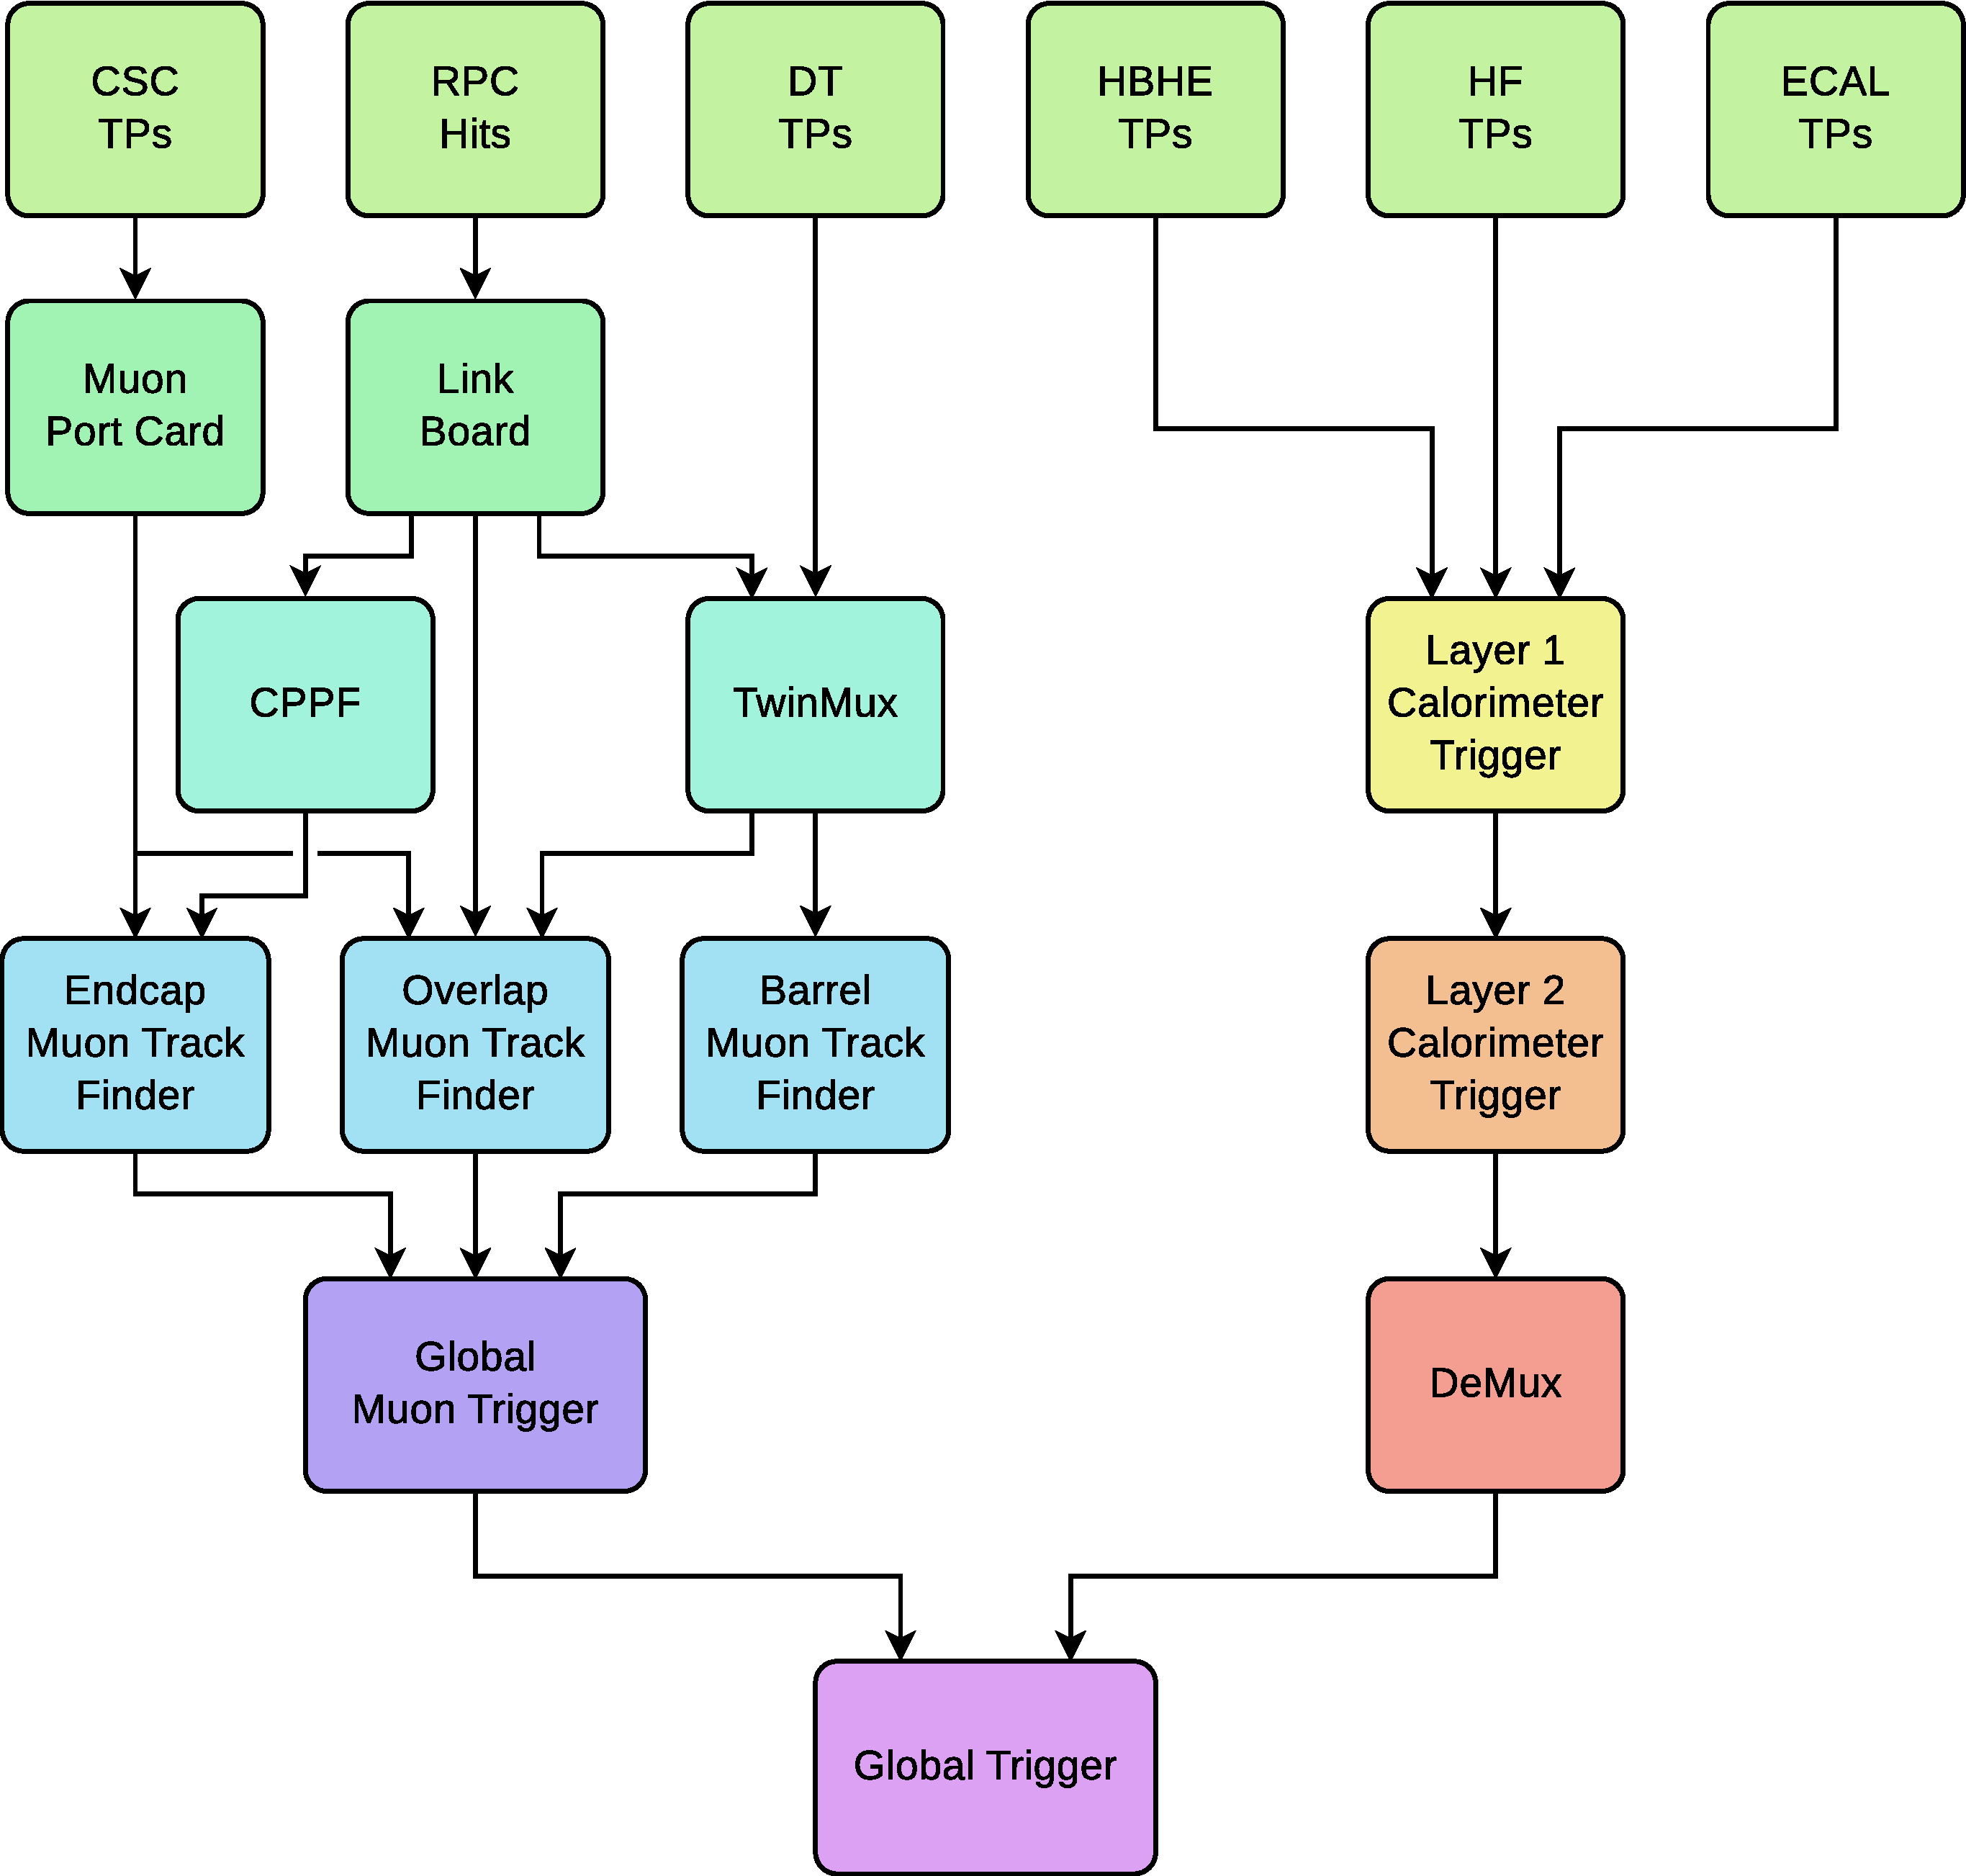
\includegraphics[width=0.75\textwidth]{Images/Trigger/CMS_L1_Trigger.pdf}
    \caption{The CMS Level-1 Trigger}
    \label{fig:CMS_L1_Trigger}
\end{figure}

It is imperative that Level-1 decisions are made in a timely fashion, quickly enough such that the on-detector electronics buffers do not fill. If this were to occur, the flow of incoming data would be halted and CMS would begin to lose events. It is for this reason that a latency of $\approx$4 $\mu$s is imposed as the maximum time limit for L1 to make a decision on whether or not to further process data from a bunch crossing (BX). 

During this $\approx$4 $\mu$s, TPs from the muon systems are input to the muon L1 algorithms: The EMTF (Endcap muon track finder), OMTF (Overlap muon track finder) and BMTF (Barrel muon track finder). These respective track finding algorithms make use of the multiple CMS muon sub-system information, and their outputs are all input to the Global Muon Trigger in order to build L1 muon objects. At the same time, the ECAL and HCAL TPs are input to the calorimeter layers: Calorimeter layers 1 and 2, which are responsible for producing L1 objects of the remaining physics objects of interest: EGamma (Electron or photon), jet, and tau objects. 

For a given event, this will result in a set of L1 objects. To determine whether or not an event passes the L1 trigger through a Level-1 accept (L1A), it is checked whether at least one of the Level-1 menu seeds meets the requirements of the event's L1 objects. If this is the case, an L1A is sent to the CMS sub-detectors in order to notify them to send the TP information stored in their on-detector electronics buffers to the central DAQ (Data acquisition) system for further processing at the HLT. It is for this reason that an appropriate level-1 menu must be designed based on the expected collisions delivered to CMS, and physics program the detector would like to pursue. 

During Run 2 and at the start of Run 3, the goal of the L1 trigger was to reduced the data-taking rate from 40 MHz to 100 kHz. 

A major update to the L1 trigger for CMS envisioned to be implemented for the Phase-II CMS detector, which will operate during the HL-LHC, is the addition of tracker information for making L1 decisions. This has the potentially to make L1 decisions based on a variety of additional physics signatures, including based on displayed vertices from b-quarks, potentially leading to much purer CMS datasets. 

\subsubsection{High Level Trigger}

% https://cms.cern/news/first-collisions-reconstructed-gpus-cms
% http://cds.cern.ch/record/2759072/files/CMS-TDR-022.pdf?version=3

After the L1 trigger makes an initial decision on which events recorded by CMS are interesting and warrant further inspection, reducing the data-taking rate from a maximum of 40 MHz to 100 kHz, events are passed to the HLT (High level trigger) to make a final decision on whether or not an event is saved at CMS. The HLT is a computing farm located above the CMS control room, which performs a reconstruction similar to the standard offline CMS event reconstruction on events passing the L1 trigger, and during Run 2 reduced the trigger rate from 100 kHz to 1 kHz for permanent storage. An image of the HLT computing farm is shown in Figure \ref{fig:HLT_Farm}.

\begin{figure}[H]
    \centering
    \includegraphics[width=0.7\textwidth]{Images/CMS/CMS_HLT_Farm.jpg}
    \caption{CMS HLT computing farm (2010)} % From 2010 
    \label{fig:HLT_Farm} % https://www.flickr.com/photos/irmp/4583961234
\end{figure}

During LS2, the CMS HLT began implementing the use of Graphical Processing Units (GPUs) in conjunction with CPUs (Central processing units) in order to decrease the time required to reconstruct physics events. The potential gain could be very useful for CMS, as if HLT processing time is decreased one would have more ``time budget'' to allocate to reconstruction, potentially allowing for more complex reconstruction, and to that end a purer dataset saved by the HLT farm. The CMS HLT is currently running with a combination of CPUs and GPUs, and has successfully commissioned this version of reconstruction for the start of LHC Run 3.  
    
    %%-- The Electromagnetic Calorimeter 
    \chapter{The CMS Electromagnetic Calorimeter}\label{chapter:ECAL}

The CMS Electromagnetic Calorimeter is the second layer of the CMS detector, with respect to the interaction point of collisions produced by the LHC. In this Chapter, the CMS ECAL will first be introduced in Section \ref{sec:ECAL_Introduction}. In Section \ref{sec:ECAL_TPG}, the method of ECAL Trigger Primitive Generation as input to the CMS L1 trigger will be described. In Section \ref{sec:DW}, the development and commissioning of a new ECAL feature known as ``Double Weights" will be described, and in Section \ref{sec:ECAL_Operations} the various ECAL operations teams and their responsibilities will be described.  

% \section{Introduction} \label{sec:ECAL_Introduction}

\subsubsection{The Electromagnetic Calorimeter}\label{sec:ECAL}

The CMS ECAL is a homogeneous crystal calorimeter composed of 75,848 PbWO$_{4}$ (lead tungstate) crystals that measures the energy of photons and electrons with high precision. The ECAL is composed of a barrel (EB) containing 61,200 crystals and covering the pseudorapidity $\eta$ region $|\eta| < 1.479$, and two endcaps (EE) containing 14,648 crystals and extending the coverage up to $|\eta| = 3$. Accurately measuring the energy and position information of electrons and photons is vital for an extensive array of physics analyses, in particular the decays of the Higgs boson in the two photon and ZZ to 4 leptons channels, considered the ``golden channels\,'' in the experimental discovery of the Higgs boson. The ECAL is supported by an additional subsystem called the ECAL Preshower (ES), located in front of each ECAL endcap. ES is composed of lead and silicon sensors, and is meant to improve two-photon separation, i.e. determine whether photons came from pion decays rather than from Higgs boson, or other interesting decays. The layout and geometry of the CMS ECAL and ES are shown in Figures \ref{fig:ECAL_Partitions} and \ref{fig:ECAL_Geometry}. Images of the EB and half of an EE endcap are shown in Figure \ref{fig:ECAL_Images}. 

\begin{figure}[H]
    \centering
    \includegraphics[width=0.65\textwidth]{Images/ECAL/Introduction/ECAL_ES_Diagram_colored.png}    
    \caption{CMS ECAL and ES partitions.}
    \label{fig:ECAL_Partitions}
\end{figure}

\begin{figure}[H]
    \centering
    \includegraphics[width=0.65\textwidth]{Images/ECAL/Introduction/ECAL_Diagram.png}    
    \caption{Geometric coverage of the CMS ECAL and ES.}
    \label{fig:ECAL_Geometry}
\end{figure}

% https://cms.cern/detector/measuring-energy/ecal-preshower

\begin{figure}[H]%
    \setcounter{subfigure}{0}
    \centering
    \subfloat[ECAL barrel]{\includegraphics[width=.4\textwidth]{Images/ECAL/Introduction/EB_Image.jpg}}%
    \hfill
    \subfloat[Half of an ECAL endcap]{\includegraphics[width=.4\textwidth]{Images/ECAL/Introduction/EE_Half.jpg}}%
    \caption{Images of the CMS ECAL. \label{fig:ECAL_Images}}%
\end{figure}  

The basis of detection at ECAL is an electromagnetic shower. As a high energy electron or photon approaches ECAL, the electron will emit a photon as bremsstrahlung radiation, and the photon will pair produce to an electron-positron pair in the presence of massive detector material. The resulting photons, electrons, and positrons from this initial process will then perform the same types of processes as a cascade of particles is produced in the ECAL crystals. This is shown as a diagram in Fig. \ref{fig:Photon_Shower} for a photon initiating a shower, Fig. \ref{fig:Electron_Shower} for an electron initiating a shower, and is visualized as a simulation in Fig. \ref{fig:Simulated_Shower}. 

\begin{figure}[H]
    \centering
    \includegraphics[width=0.7\textwidth]{Images/ECAL/Introduction/Photon_Shower.png}    
    \caption{Diagram form of a photon initiating an electromagnetic shower via pair production of an electron-positron pair.}
    \label{fig:Photon_Shower}
\end{figure}

\begin{figure}[H]
    \centering
    \includegraphics[width=0.7\textwidth]{Images/ECAL/Introduction/Electron_Shower.png}    
    \caption{Diagram form of an electron initiating an electromagnetic shower via bremsstrahlung radiation.}
    \label{fig:Electron_Shower}
\end{figure}

\begin{figure}[H]
    \centering
    \includegraphics[width=0.7\textwidth]{Images/ECAL/Introduction/EM_Crystal_Shower.png}    
    \caption{Simulated electromagnetic shower inside a material.}
    \label{fig:Simulated_Shower}
\end{figure}

In ECAL, this EM shower leads to scintillation in its lead tungstate crystals, producing light that is read by photodetectors on the back of the crystals. The EB uses APDs (avalanche photodiodes), and the endcaps use VPTs (vacuum phototriodes) to convert scintillation light into an electrical signal. Digitized samples of ECAL are taken every 25 ns, and through a series of calibrations, the samples can be converted into an energy in GeV. An image of an EE crystal with its attached VPT is shown in Figure \ref{fig:ECAL_XTAL}.

% https://indico.cern.ch/event/1002959/contributions/4211462/attachments/2192922/3706736/EGM_Seminar_21-02-18.pdf

\begin{figure}[H]
    \centering
    \includegraphics[width=0.7\textwidth]{Images/ECAL/Introduction/SC_VPT_and_crystal.jpg}    
    \caption{EE crystal with its attached VPT.}
    \label{fig:ECAL_XTAL}
\end{figure}
\section{Trigger primitive generation} \label{sec:ECAL_TPG}

ECAL provides an input to the CMS Level-1 trigger in the form of trigger primitives. It is one of several inputs to the CMS Level-1 trigger, as shown in Figure \ref{fig:CMS_L1_Trigger}. This section is structured as follows: Section \ref{sec:ECAL_TP} will describe the composition of ECAL trigger primitives, and section \ref{sec:PU_Optimized_Weights} will describe a re-optimization of ECAL TP generation, known as PU optimized weights.  

\subsection{ECAL trigger primitives} \label{sec:ECAL_TP}

ECAL TPs are one of three inputs into the Layer 1 Calorimeter Trigger, shown in Figure \ref{fig:CMS_L1_Trigger}. The basic building blocks of ECAL TPs, with the Phase-I electronics used during LHC data-taking, are ``strips" composed of 5 crystals each in EB, and 1-5 crystals in EE. Every 25 ns, a digitized sample is taken of ECAL signals in every crystal, shown in Figure \ref{fig:ECAL_Waveform_Digis}. During data taking, this leads to a constant stream of values measured in ADC (analog to digital converter) counts. These values are linearized to account for different gains that may be set in different amplifiers, summed within a strip. For each set of 10 linearized strip samples, a digital filter made of a set of 10 FIR (Finite impulse response) weights is multiplied by their corresponding sample values and summed to obtain a transverse energy ($E_{T}$) value, shown in Equation \ref{eq:weights_equations}. In this equation, $S_{i}$ represents digitized sample ``i", where ``i" can range from 0-10 for the 10 digitized samples taken from an ECAL pulse from 0-225ns. Additionally, $w_{i}$ represents the FIR weight assigned to sample ``i", which is pre-determined for each ECAL strip. A requirement on the FIR weights is that they sum to zero, in order to include a dynamic pedestal subtraction, also shown in Equation \ref{eq:weights_equations}. This is performed for every subsequent set of 10 samples, with the window of 10 samples shifting 25ns forward each time, leading to a constant stream of $E_{T}$ values. Additionally, a peak finder is then applied to strip sums in order to determine which BX (Bunch crossing) in a predefined window of BXs has the greatest calculated $E_{T}$ value. Strip energies are then summed to form trigger towers (5 strips in EB, 1-5 strips in EE), for which TPs are formed. An ECAL TP is an $E_{T}$ value of a trigger tower at a given BX, with up to two feature bits. One feature bit is the fine grain bit, and is used to distinguish EM signals from jets. In EB TPs, a bit is also reserved for the rejection on anomalous signals termed ``spikes". When a BX has a TP created, the other BXs in the window are not eligible to have a TP formed. Non-zero TPs are sent to TCC (Trigger concentrator card) boards for further processing and time alignment before being sent to the L1 trigger. A schematic showing this process and computation of strip $E_{T}$ is shown in Figure \ref{fig:ECAL_TP_Formation}.

\begin{figure}[H]
    \centering
    \includegraphics[scale=0.5]{Images/ECAL/TPG/EM_Waveform_Example.pdf}
    \caption{ECAL analog pulse shape example, with digitized samples taken every 25ns.}
    \label{fig:ECAL_Waveform_Digis}
\end{figure}

\begin{equation} \label{eq:weights_equations}
E_{T} = \sum_{i=1}^{10}S_{i}\times w_{i}
   \quad\text{,}\quad 
\sum_{i=1}^{10}w_{i} = 0 
\end{equation}

\begin{figure}[H]
    \centering
    \includegraphics[width=\textwidth]{Images/ECAL/TPG/XTAL_To_ET.png} \caption{ECAL strip $E_{T}$ formation.}
    \label{fig:ECAL_TP_Formation}
\end{figure}

Each ECAL TP in EB and EE is composed of an $E_{T}$ value computed as the sum of its strip $E_{T}$ values, information bits, and a BX assignment. ECAL TPs are created on-detector, and are transmitted to the Level-1 trigger at the LHC collisions rate of 40 MHz. Because the transverse momentum of two LHC proton bunches before colliding is 0, the detection of hits with a high $E_{T}$ or \pt component is a potential sign of an interesting hard interaction between protons, and thus is a quintessential quantity to consider when forming an L1 decision.  

\subsection{PU optimized weights} \label{sec:PU_Optimized_Weights}

Throughout Runs 1 and 2, two sets of amplitude weights were used when computing ECAL strip energies and hence TP energies, one for EB and one for EE, shown in Figure \ref{fig:ECAL_weights}.

\begin{figure}[H]
\begin{center}
\begin{tabular}{ccccccccccc} \toprule

sample & 1 & 2 & 3 & 4 & 5 & 6 & 7 & 8 & 9 & 10 \\ \midrule
EB & 0 & 0 & -0.5625 & -0.546875 & 0.25 & 0.484375 & 0.375 & 0 & 0 & 0 \\ EE & 0 & 0 & -0.65625 & -0.515625 & 0.25 & 0.515625 & 0.40625 & 0 & 0 & 0 \\ \bottomrule

\end{tabular} 
\end{center}
\caption{Run 1 and 2 ECAL FIR weights} % \cite{DPG_Slides}
\label{fig:ECAL_weights}
\end{figure}

These FIR weight values were obtained from ECAL pulse shapes measured in test beams, as for a given waveform shape, an optimal set of weights can be extracted for measuring the waveform's height.

One way to simulate the photo-detectors' response to crystal scintillation is with an analytic waveform. The function used to simulate the time evolution of the detector response for each crystal is the alpha-beta function defined in Equation \ref{eq:alphaBetaFunction}. 

\begin{equation} \label{eq:alphaBetaFunction}
	f(t) = 	
	\begin{cases} 
      f(t) = A*\Bigg(1 + \dfrac{(t - t_{0})}{(\alpha\beta)}\Bigg)^{\alpha}*e^{\frac{-(t-t_{0})}{\beta}} & t > (t_{0} - \alpha*\beta) \\
     0 & t \leq (t_{0} -\alpha*\beta)
  \end{cases}
\end{equation}

In this equation, A is the height of the waveform in ADC counts, $t_{0}$ is the time of the waveform's peak in nanoseconds, $\alpha$ describes the behavior of the polynomial term, and $\beta$ corresponds to the decay time in the exponential term. The pedestal (P) can also be set, giving the full analytic form of the detector response shown in Equation \ref{eq:FullECALresponsefcn}.

\begin{equation} \label{eq:FullECALresponsefcn}
G(t;P) = f(t)+P
\end{equation}

With dedicated fine grain time scans performed on ECAL signals, the parameters $A$, $t_{0}$, $\alpha$ and $\beta$ were measured for each crystal during Run 2. These scans were performed in October 2017, June 2018, and September 2018, and a variation of the parameters among the crystals can be seen over time due to the ageing of ECAL crystals caused by steady dosages of radiation from LHC collisions. 

By producing and sampling these waveforms and applying the Run 2 FIR weights to the samples, one can simulate the reconstructed amplitude of the ECAL TPs as a function of pseudorapidity ($\eta$). A fractional amplitude bias, defined as the percent difference between the reconstructed amplitude, $\hat{A}$ and the true amplitude $A$ and shown in Equation \ref{eq:bias}, is shown as a function of $\eta$ in Figure \ref{fig:ampBiasvseta} \cite{CMS-DP-2019-031, CMS-DP-2019-031_Plots}. 

\begin{equation} \label{eq:bias}
    \text{bias} = \frac{\hat{A}}{A} - 1
\end{equation}

\begin{figure}[H]
    \centering
    \includegraphics[width=\textwidth]{Images/ECAL/TPG/AmpBias_vs_eta_Sep18_ps.pdf}
    \caption{Average bias vs. $\eta$, with no simulated time shift (ts = 0ns), using September 2018 parameters for detector response and Run 2 weights for reconstruction.}
    \label{fig:ampBiasvseta}
\end{figure}

It can be seen from this result that there is a bias in the reconstructed amplitude, particularly in the high-$\eta$ region where a greater average and spread of bias is present. In the high-$\eta$ region occupied by the EE, the average fractional amplitude bias is about a factor of three larger than that in the EB region. This is consistent with the fact that ECAL crystals in the high-$\eta$ region receive more radiation from LHC collisions, and therefore their crystals and corresponding waveforms are more distorted and stray further from their original shapes use to derive their FIR weights. This indicates that a more ideal set of weights can be produced in order to produce more accurate TPs. This motivates the derivation of new amplitude weights to see if a reduction in bias average and spread can be made. 

In order to derive updated amplitude weights, a simulation of ECAL electronics' response to scintillation light was setup from the most recent timing scan data obtained in September 2018, including a realistic PU scenario which depends on $\eta$, and distorts the in-time ECAL pulses. Using the alpha-beta analytic waveform to model each crystal's response, and taking a realistic PU energy spectrum and LHC proton bunch train into account (48b7e), the fractional spread of energy biases was computed as a function of signal BX shown in Figure \ref{fig:gr_train_nonzero_Asf_48b7e_0_8_std} for ECAL EB crystals with $|\eta| < 0.7$, and for EE crystals with $2.3 < |\eta| < 3.0$ in Figure \ref{fig:gr_train_nonzero_Asf_48b7e_26_28_std} \cite{CMS-DP-2022-016, CMS-DP-2022-016_Plots}

\begin{figure}[H]
    \centering
    \includegraphics[width=\textwidth]{Images/ECAL/TPG/gr_train_nonzero_Asf_48b7e_0_8_std.pdf}
    \caption{Fractional spread of amplitude bias for simulated ECAL crystal responses in the region $|\eta| < 0.7$.}
    \label{fig:gr_train_nonzero_Asf_48b7e_0_8_std}
\end{figure}

\begin{figure}[H]
    \centering
    \includegraphics[width=\textwidth]{Images/ECAL/TPG/gr_train_nonzero_Asf_48b7e_26_28_std.pdf}
    \caption{Fractional spread of amplitude bias for simulated ECAL crystal responses in the region $2.3 < |\eta| < 3.0$.}
    \label{fig:gr_train_nonzero_Asf_48b7e_26_28_std}
\end{figure}

For both ECAL regions, fractional spread is shown when reconstructing amplitude with the Run 2 weights, PU optimized weights optimized for a strip $E_{T}$ of 2 GeV, and for a strip $E_{T}$ of 30 GeV. In the EB region, an improvement in fractional spread of about 1\% is obtained with respect to Run 2 weights when using weights optimized for PU and $E_{T}$ = 2 GeV. In EE, a more drastic improvement of about 15-20\% is obtained with respect to Run 2 weights. This is consistent with Figure \ref{fig:ampBiasvseta}, which shows there is more room for improvement in EE compared to EB. 

This indicates that updating the existing EB and EE FIR weights may improve the spread of fractional bias in TP $E_{T}$ computation. The effect of updated ECAL TP FIR weights on Level-1 quantities, and further evaluation of the potential gain from updating the ECAL L1 amplitude weights to account for changes in ECAL pulse shapes due to ageing and PU is currently being studied and tested in an effort to improve ECAL for Run 3. A potential positive impact of improved ECAL TP resolution is an increase in the L1 tagging efficiency of electron and photon objects, which can potentially increase the efficiency of triggering on HH$\rightarrow$WW$\gamma\gamma$ events, and events with similar signatures, at the CMS detector. 

In addition to amplitude weights, sets of timing sensitive weights can also be derived. Instead of returning an amplitude when multiplied by waveform samples, these return timing jitter, defined as the time displacement from the expected peak time. These ideal sets of weights are derived to return a bias of 0 when the input waveform is the one they were derived from. Therefore, the effectiveness of these two types of weights can be shown by plotting their bias when different time shifts are applied, defined as a translation of the waveform left or right. For example, a time shift of 5 ns means $t_{0}$ would go from $t_{0}$ to $t_{0} + 5ns$. The average fractional amplitude and time biases as a function of time shift are shown in Figures \ref{fig:ampBiasvsTimeShift} and \ref{fig:timeBiasvsTimeShift}. 

\begin{figure}[H]%
    \centering
    \subfloat[Average amplitude bias vs. time shift \label{fig:ampBiasvsTimeShift}]{\includegraphics[width=0.8\textwidth]{Images/ECAL/TPG/AmpBias_vs_ts_Sep18_Id.pdf}}%
    \\ \newline 
    \subfloat[Average timing bias vs. time shift \label{fig:timeBiasvsTimeShift}]{\includegraphics[width=0.8\textwidth]{Images/ECAL/TPG/TimeBias_vs_ts_Sep18_Id.pdf}}%
    \caption{(a) Amplitude and (b) time bias vs time shift for ECAL waveforms, using September 2018 parameters for detector response and ideal weights for reconstruction, for crystals in the $\eta$ region: $(-3.0,-2.6)$}%
\end{figure}

For time shifts of 0, there is no bias in amplitude or timing weights because the weights were derived for each non-time-shifted waveform. Because the bias is not large for small time shifts, ideal weights can be considered worth investigating. 

\section{Double weights} \label{sec:DW}

Throughout LHC Runs 1 and 2, the on-detector ECAL FENIX chip, a custom ASIC, was used for energy reconstruction to form $E_{T}$ sums for ECAL TPs, multiplying one set of weights by recorded digis as described in Section \ref{sec:ECAL_TP}. During LS2, it was discovered that the ECAL FENIX chip has the capacity to store and use two sets of weights. This essentially duplicates the ECAL FENIX data path, as shown in Figure \ref{fig:DW_Diagram}, into two electronically equivalent paths, one for each FIR filter named the ``EVEN" and ``ODD" filters.

\begin{figure}[H]
    \centering
    \includegraphics[width=\textwidth]{Images/ECAL/DW/ECAL_DW_Schematic.png}
    \caption{ECAL double weights mechanism.}
    \label{fig:DW_Diagram}
\end{figure}

This feature was implemented in the ECAL FENIX chip for potential further use, but was never used during Runs 1 and 2. 

\subsection{Spikes} \label{sec:spikes}

A commonly observed phenomenon at the ECAL is the direct ionization of the ECAL EB APDs, which produce anomalous signals termed ``spikes". Because these signals do not come from electromagnetic showers originating from the hard interactions of LHC collisions, they must be removed as efficiently as possible to keep trigger rates under control and preserve the quality of the offline reconstruction of electrons, photons and jets. Additionally, spike progenitors often spend time propagating in the CMS detector before directly ionizing the EB APDs, and therefore may be out-of-time with respect to electromagnetic signals.

There is a method in place used to remove spikes at L1 using a topological cut, termed the ``spike killer" \cite{Petyt_2012}. This operates by making a topological cut, exploiting the fact that spikes typically deposit all of their energy into a single ECAL crystal as they are due to the direct ionization of APDs, while EM showers are expected to be spread among multiple crystals. A diagram showing the mechanism of the spike killer is shown in Figure \ref{fig:spikeKillerDiagram}. 

\begin{figure}[H]
    \centering
    \includegraphics[width=\textwidth]{Images/ECAL/DW/SpikeKillerDiagram.png}
    \caption{Operation of the strip Fine-Grained Veto Bit (sFGVB) on an electromagnetic shower (left) and a spike-like energy deposit (right).}
    \label{fig:spikeKillerDiagram}
\end{figure}

The spike killer makes use of a per-strip bit, the strip Fine-Grained Veto Bit (sFGVB) which is set to 1 if at least 2 crystals in a strip are above a per-crystal energy threshold. If a trigger tower (set of 25 crystals, 5 strips) has at least one strip with a sFGVB equal to 1, it is preserved as it is considered EM shower-like due to its spread in energy. However, if a TT has no strips with at least one sFGVB set to 1, the TP energy is set to 0 if its energy is above the spike killer ``killing threshold" of 16 GeV. 

In order to optimize the spike killer for Run 3 where higher noise and everage PU is expected, the per-crystal energy threshold was increased, as there will be a higher expected contribution from noise and PU for all crystals. The spike contamination among TPs with the Run 2, and candidate Run 3 working point is shown in Figure \ref{fig:spikeKillerRun3optimization}. Notably in this spike contamination plot, produced using data from a ZeroBias dataset (no triggering on typical physics menus), there is a high spike contamination at high energy. This is because it is more likely to produce a high energy spike, which are high energy due to its direct ionization of the APDs, than a high energy EM shower, which requires the production of a truly high energy particle from proton-proton interactions. 

\begin{figure}[H]
    \centering
    \includegraphics[width=0.8\textwidth]{Images/ECAL/DW/spikekiller_run3_optimisation.pdf}
    \caption{Spike fraction vs. TP $E_{T}$ threshold with a Run 2, and Run 3 candidate working point of the existing ECAL L1 spike killer. The data comes from a ZeroBias dataset recorded in July 2018 with a peak pileup of 50.}
    \label{fig:spikeKillerRun3optimization}
\end{figure}

This shows that while updating the settings of the existing spike killer to a candidate Run 3 working point removes additional spikes at Level-1, there is much room for improvement, especially in the high energy regime. Additionally, at L1 there is no existing spike killer in the low energy regime 0-16 GeV, as this is below the spike killer threshold. 

\subsection{Timing weights}

The initial idea for optimizing ECAL double weights was to keep the original set of amplitude weights in the EVEN filter, and to utilize the second set of weights, the ODD filter, as a set of timing weights in order to compute an on-detector timing value for trigger primitives. These studies showed possible discrimination power, as the timing weights were able to identify out of time signals which came from spikes. Figures \ref{fig:ampvstime_EMlike} and \ref{fig:ampvstime_Spikelike} show the reconstructed amplitude computed as the EVEN weights times signal digis, vs. the reconstructed time as computed by multiplying a set of optimal timing weights occupying the ODD filter by signal digis for signal and spike-like TPs in CMS data. 

\begin{figure}[H]
    \centering
    \includegraphics[width=0.8\textwidth]{Images/ECAL/DW/EM_TPs.pdf}
    \caption{Reco amplitude vs. Reco time of EM-like signals in CMS data}
    \label{fig:ampvstime_EMlike}
\end{figure}

\begin{figure}[H]
    \centering
    \includegraphics[width=0.8\textwidth]{Images/ECAL/DW/Spike_TPs.pdf}
    \caption{Reco amplitude vs. Reco time of spike-like signals in CMS data}
    \label{fig:ampvstime_Spikelike}
\end{figure}

By eye, most EM-like signals fall within a reconstructed time window near zero, with a tail going out to around 20 ns for signals with a greater reconstructed amplitude. For spike-like signals, there is a larger time window with some TPs very out-of-time. Interestingly, in the EM-like signals on Figure \ref{fig:ampvstime_EMlike} one can see a low population line of entries which appears to follow the trend of the spike-like signals in Figure \ref{fig:ampvstime_Spikelike}, as these are possibly real spikes which are incorrectly tagged offline as signal-like. 

For the sake of quantifying the possible discrimination power of ECAL timing weights, a hypothetical timing cut of -5 $<$ t $<$ 20 ns would have been able to drastically reduce the rate of spikes, as shown in Figure \ref{fig:TimingCutSpikeReduction}.

\begin{figure}[H]%
    \setcounter{subfigure}{0} % reset subcaption counter to 0 (a) 
    \centering
    \subfloat[Spike Rates]{\includegraphics[width=0.49\textwidth]{Images/ECAL/DW/spikeTPet_beforeaftertimingcut.pdf}}%
    %\qquad
    \subfloat[Spike Fractions]{\includegraphics[width=0.49\textwidth]{Images/ECAL/DW/spikecontamination_beforeaftertimingcut.pdf}}%
    \caption{Spike quantities with/without timing cut \href{https://twiki.cern.ch/twiki/bin/view/CMSPublic/EcalDPGResultsCMSDPS2019031}{[EcalDPGResults]},\href{https://cds.cern.ch/record/2690933/files/DP2019_031.pdf}{[CDS]}}%
    \label{fig:TimingCutSpikeReduction}
\end{figure}     

A timing cut like this is not possible in the ECAL FENIX chip; However this study motivated the idea to use two sets of amplitude weights and a comparator in the FENIX chip in order to identify out-of-time signals with double weights. 

\subsection{Optimization}

In the ECAL FENIX chip, it is possible to compute two amplitudes via two sets of weights, and utilize a comparator in the electronics to set a boolean flag if one amplitude output is greater than the other. If an ODD set of weights is optimized to identify out of time signals, it is expected to returns a greater amplitude for out-of-time signals than the Run 2 weights designed for in-time signals. Therefore, the approach is taken to optimize an ODD set of weights for out-of-time signals.

Choosing an odd set of weights for out-of-time signal tagging is a multivariate problem, which must consider a realistic signal energy spectrum, spike energy spectrum, spike timing PDF, and the effects of pileup on signal waveform distortion. Therefore in order to extract ODD weights sets which are optimized to maximize signal efficiency and spike rejection, a numerical optimization was setup in order to derive optimal sets of weights to take the place of the second FIR filter weights. This optimization makes use of simulated signal waveforms using the alpha-beta analytic representation and simulated pileup described in Section \ref{sec:PU_Optimized_Weights}, and the simulation of spike waveforms from a standalone simulation. The optimization is setup as a loss minimization problem which makes use of gradient descent computation and backwards propagation of loss to maximize the amount of spike rejection, while minimizing the amount of signal rejection. This is incorporated in a loss definition, shown in Figure \ref{fig:NumOptLoss}.

\begin{figure}[H]%
    \setcounter{subfigure}{0} % reset subcaption counter to 0 (a) 
    \centering
    \subfloat[Loss function]{\includegraphics[width=0.31\textwidth]{Images/ECAL/DW/LossFunction.png}}%
    \hfill
    \subfloat[Use of $\delta_{min}$ in loss]{\includegraphics[width=0.31\textwidth]{Images/ECAL/DW/deltamin_use.png}}%
    \hfill
    \subfloat[Definition of ODD weights loss limit.]{\includegraphics[width=0.31\textwidth]{Images/ECAL/DW/W2LossLimit.png}}
    \caption{Loss definition used in optimization of ODD set of amplitude weights.}%
    \label{fig:NumOptLoss}
\end{figure}  

One of the input parameters in the optimization is a minimum separation of the two amplitude values computed by the EVEN (default weights) and ODD (out-of-time sensitive) sets of weights, termed $\delta_{min}$. Varying this parameter results in different working points. The different portions of a simulated spike timing PDF which were tagged as out of time by different working points is shown in Figure \ref{fig:DW_StandaloneSimulation_SpikeTimingPDFTagging} \cite{CMS-DP-2022-007, CMS-DP-2022-007_Plots}. 

\begin{figure}[H]
    \centering
    \includegraphics[width=0.8\textwidth]{Images/ECAL/DW/Double_Amplitude_Weights_SpikeTaggingwithOOTWeights_allDeltaMins.pdf}
    \caption{Tagging of out of time spikes in a standalone simulation.}
    \label{fig:DW_StandaloneSimulation_SpikeTimingPDFTagging} 
\end{figure}

In the spike timing PDF, most spikes are relatively in-time with respect to EM signals, while a non-negligible fraction have a late out of time tail. The reason for this is because spike progenitors often spend time propagating in the CMS detector before directly ionizing the EB APDs. It can be seen that increasing the value of the $\delta_{min}$ parameter tags later out of time spikes. This is somewhat expected, as a larger $\delta_{min}$ value will only use spike examples with larger differences in EVEN and ODD amplitudes in its optimization, which is more likely to come from out-of-time shifted spikes. 

While quantifying the expected gain in spike rejection from different $\delta_{min}$ working points, it is also important to check their effect on EM shower-like signals, as shown for a standalone simulation in Figure \ref{fig:SimSignaltaggedvsE}. 

\begin{figure}[H]
    \centering
    \includegraphics[width=0.8\textwidth]{Images/ECAL/DW/SigEff_vs_SigET.pdf}
    \caption{Signal efficiency vs. signal energy using a standalone simulation and simulation of ECAL double weights algorithm.}
    \label{fig:SimSignaltaggedvsE}
\end{figure}

It is observed that increasing the $\delta_{min}$ parameter value results in higher signal efficiency, as expected for the same reason that a greater spike rejection is observed for greater $\delta_{min}$ values: Only signal and spike waveforms which exhibit larger differences in EVEN and ODD amplitudes are used for weight optimization, leading to weights which are more optimized for very different waveforms and therefore less likely to touch signal waveforms. In order to identify a reasonable trade-off between signal efficiency and spike rejection, the resulting efficiencies are rejections for different $\delta_{min}$ working points is shown in Figure \ref{fig:SpikeRejSigEffTable}, where only signals with $E_{T} \leq 3$ GeV are considered as simulated signals with $E_{T} > $ 3 GeV have an efficiency near 100\%. Additionally, only spikes with a timing greater than 10 ns are considered, as these working points are not effective at tagging in-time spikes.

\begin{figure}
    \centering
        \begin{tabular}{|c|c|c|} \hline 
          $\delta_{min}$ (GeV) & Signal efficiency (\%) & Spike rejection (\%) \\ \hline 
         0.5 & 78.2 & 77.6 \\ \hline  
         2.5 & 95.6 & 62.5 \\ \hline 
         5.0 & 95.7 & 19.2 \\ \hline    
        \end{tabular}
    \caption{Signal efficiency and spike rejection for different $\delta_{min}$ working points.}
    \label{fig:SpikeRejSigEffTable}
\end{figure}

It is shown that moving from the $\delta_{min} = $ 2.5 GeV to 5.0 GeV working point returns a minimal gain in signal efficiency (0.1\%), while a large fraction of spike
rejection is lost (43.3\%). This indicates that the $\delta_{min} = 2.5$ GeV working point provides a good compromise between signal efficiency at low $E_{T}$ and overall spike rejection.

\subsection{Re-emulation of 2018 data} \label{sec:reEmuOf2018Data}

One of the ways to test new features during a long shutdown period when no new data is being taken is be re-emulating previously recorded data. As double weights were an undiscovered feature, they were not present in the CMS ECAL emulator. After verifying the existence of this feature in hardware through tests at CERN building 904 and at the CMS ECAL itself, the now confirmed second amplitude filter was added as a possible configuration in the CMS emulator \cite{CMSSW_DW}.

After including this implementation in the centrally used CMS software, 2018 CMS data was re-emulated using ECAL double weights in order to see how this would have affected data-taking. Double weights were run in "Killing mode", meaning that if an ECAL strip has a higher ODD amplitude than EVEN amplitude, its energy is set to zero. The idea behind this is to zero spikes which are often out-of-time, while trying to minimize the zeroing of signals which are in-time. 

In order to categorize ECAL TPs in data as signal-like or spike-like, an offline ``Severity" assignment is used. Each EB TT (Trigger tower) is composed of 25 ECAL crystals. An offline energy computation is performed for each crystal in highly energetic regions of events with an L1A, called a reconstructed hit or ``rec hit". In addition, a timing value is computed for each reconstructed hit, and a ``severity" level is assigned. A severity level of 0 corresponds to a reconstructed hit which does not appear problematic in the data. A severity level of 3 means a reconstructed hit is identified as out-of-time based on its reconstructed timing value, and a severity level of 4 means a reconstructed hit satisfies at least one of the following: Identified as out-of-time based on its reconstructed time value, fails a topological cut, known as a ``swiss-cross" cut. Because spikes come from isolated APD hits, rather than from a spread-out EM shower with energy spread over a group of ECAL crystals, spikes usually have their energy fully deposited in one crystal and are identified using a swiss cross variable, shown in Figure \ref{fig:SwissCross}. Thus, severity zero (four) reconstructed hits typically correspond to signal-like (spike-like) hits shown in its respective region of reconstructed time vs. swiss-cross score in Figure \ref{fig:TimeVsSwissCross} \cite{CMS-DP-2012-008, CMS-DP-2012-008_Plots}. 

\begin{figure}[H]%
    \setcounter{subfigure}{0}
    \centering
    \subfloat[Swiss cross definition, illustrated by the energy hits in a 3x3 ECAL crystal portion. E1 = energy of the central crystal, E4 = sum of the energies of the central crystal's four surrounding neighbors.  \label{fig:SwissCross}]{\includegraphics[width=.475\textwidth]{Images/ECAL/DW/SwissCross.png}}%
    \hfill
    \subfloat[Reconstructed time vs. swiss cross score \label{fig:TimeVsSwissCross}]{\includegraphics[width=.475\textwidth]{Images/ECAL/DW/timeVsSwissCross.png}}%
    \caption{Swiss cross definition, and reconstructed hit timing vs. swiss cross score from a 2010 CMS data sample.}%
\end{figure}

In order to assign a severity level and reconstructed time to an EB TP, the severity level and reconstructed time of the highest energy reconstructed hit in a given TP is assigned to that TP, as shown in Figure \ref{fig:RecHitTPMatching}. In this example TP with reconstructed crystal energies in arbitrary units, the highest energy reconstructed hit is in Strip 3, crystal 0 as its value is 201, and thus this TP is assigned the timing and severity of this crystal. 

\begin{figure}[H]
    \centering
    \includegraphics[width=0.8\textwidth]{Images/ECAL/DW/TPRecHitMatching.png}
    \caption{Reconstructed hit matching to TP. Crystal energy units are arbitrary.}
    \label{fig:RecHitTPMatching}
\end{figure}

In the re-emulation of 2018 CMS data, the resulting 1 - emu/real distributions, where emulated energy includes double weights in killing mode, and real energy corresponds to the energy of the TP from data with no double weights applied, are shown in Figure \ref{fig:2018Reemulation_KillingMode} for signals (TPs assigned to severity 0 reconstructed hits) which are in time (matched reconstructed crystal hit time $|t| < 3$ns), and spikes (TPs assigned to severity 4 reconstructed hits) which are out-of-time (matched reconstructed crystal hit time $t > 10$ns). 

\begin{figure}[H]%
    \setcounter{subfigure}{0}
    \centering
    \subfloat[2018 CMS data re-emulation, in time severity zero energies in killing mode \label{fig:DW_2018Reemulation_InTimeSevZeroKillingMode}]{\includegraphics[width=.475\textwidth]{Images/ECAL/DW/DW_2018_Reemulation_InTimeSevZeroEnergies.png}}%
    \hfill
    \subfloat[2018 CMS data re-emulation, very late severity four energies in killing mode \label{fig:DW_2018Reemulation_VeryLateSevFourKillingMode}]{\includegraphics[width=.475\textwidth]{Images/ECAL/DW/DW_2018_Reemulation_VeryLateSevFourEnergy.png}}%
    \caption{2018 Data reemulation with double weights in killing mode. \label{fig:2018Reemulation_KillingMode}}%
\end{figure}

This shows that relatively high energy spikes, greater than about 50 ADC (25 GeV), are being mostly zeroed, shown by the fact that the 1 - emulated / real is close to one, meaning the emulated (TP energy with double weights in killing mode) energy is nearly zeroed. There is also a non-negligible amount of zeroing being applied to in-time signals, as the per y-slice distributions show some entries greater than 0. 

To check the timings of TPs which have some energy subtracted by double weights in the full timing range, not just restricted to in time and very later, we can observe the data TP vs. its offline assigned time for all TPs shown in Figures \ref{fig:All_Sev_zero} and \ref{fig:All_Sev_four}, and for TPs in which at least 90\% of energy is removed by double weights in killing mode in figures \ref{fig:MostlyZeroed_Sev_zero} and \ref{fig:MostlyZeroed_Sev_four}. For both severity categories, a line is drawn at 32 ADC, equivalent to 16 GeV for ECAL TPs, as this is the spike killing threshold as defined in Section \ref{sec:spikes}. 

\begin{figure}[H]%
    \setcounter{subfigure}{0}
    \centering
    \subfloat[All severity zero TPs \label{fig:All_Sev_zero}]{\includegraphics[width=.475\textwidth]{Images/ECAL/DW/DW_2018_Reemulation_AllSevZeroTPs.png}}%
    \hfill
    \subfloat[Severity zero TPs mostly zeroed \label{fig:MostlyZeroed_Sev_zero}]{\includegraphics[width=.475\textwidth]{Images/ECAL/DW/DW_2018_Reemulation_SevZeroTPsMostlyZeroed.png}}%
    \caption{2018 Data reemulation - severity 0 TPs \label{fig:A}}%
\end{figure}

\begin{figure}[H]%
    \setcounter{subfigure}{0}
    \centering
    \subfloat[All severity four TPs \label{fig:All_Sev_four}]{\includegraphics[width=.475\textwidth]{Images/ECAL/DW/DW_2018_Reemulation_AllSevFourTPs.png}}%
    \hfill
    \subfloat[Severity four TPs mostly zeroed \label{fig:MostlyZeroed_Sev_four}]{\includegraphics[width=.475\textwidth]{Images/ECAL/DW/DW_2018_Reemulation_SevFourTPsMostlyZeroed.png}}%
    \caption{2018 Data reemulation - severity 4 TPs \label{fig:A}}%
\end{figure}

In the distributions containing all TPs, most signals are in-time as expected. It is also observed that a large portion of spikes are out of time, as expected. It is observed that many spikes have a negative timing around -12.5ns, which is due to a bias in the ECAL offline energy reconstruction, which is optimized for signal waveforms which are slightly different from spike waveforms. Spike waveforms with a negative reconstructed time are generally expected to really be in time. Additionally, the effect of the spike killer is visible for severity four TPs, as there is a sharp drop-off in the number of TP entries above the spike killer threshold of 32 ADC (16 GeV). 

The distributions of TPs which have at least 90\% of their energy subtracted by double weights in killing mode show that most signal-like TPs which are mostly zeroed are very low energy and out of time, which are likely coming from noise, and it can be seen that there is a non-zero chance of some in-time signal energy subtraction. For spike TPs, it is seen that the majority of TPs which have their energy mostly subtracted are positively out of time, as expected with double weights based on the standalone simulation shown in Figure \ref{fig:DW_StandaloneSimulation_SpikeTimingPDFTagging}. The spike contamination of ECAL TPs, with and without double weights activated in killing mode, is shown in Figure \ref{fig:DW_2018Reemulation_SpikeContamination}. 

\begin{figure}[H]
    \centering
    \includegraphics[width=0.8\textwidth]{Images/ECAL/DW/SpikeContamination_DoubleWeights.png}
    \caption{2018 CMS data re-emulation, expected improvement in spike contamination, including below the spike killer threshold.}
    \label{fig:DW_2018Reemulation_SpikeContamination}
\end{figure}

This shows that with ECAL double weights, there is some potential to lower the spike contamination rate, including in the high energy regime. This is also true for spikes with energy less than 32 ADC (16 GeV), the existing Level-1 spike killer threshold. 

While we see potential for a decrease in spike contamination, this re-emulation of 2018 CMS data also showed we may expect to have the unwanted removal of some signal energy at low TP energies with this double weights working point. In order to further study this, another re-emulation was performed with a full-readout ECAL run. The reason a full-readout run was included in this study is because in full-readout, information from all ECAL crystals is saved. In non full-readout runs, there is a selective readout procedure in which low interest regions are not readout. It is desirable to re-emulate full readout runs when comparing low energy TP energies between data and re-emulation, to ensure that all ECAL information is available for emulation in order to have a proper comparison to data. This re-emulation was performed with two double weights working points: $\delta_{min}$ = 0.5 and 2.5 GeV, running with double weights in killing mode. The resulting average energy fractions subtracted from in time signals and out-of-time spikes when re-emulating with these two working points are shown in Figure \ref{fig:2018Reemulation_FR_KillingMode_deltamincompare}. 

\begin{figure}[H]%
    \setcounter{subfigure}{0}
    \centering
    \subfloat[In time severity zero TPs \label{fig:2018Reemulation_FR_KillingMode_deltamincompare_InTimeSignals}]{\includegraphics[width=.475\textwidth]{Images/ECAL/DW/Sev_zero_inTime_Average_oneMinusEmuOverRealvstwrADCCourseBinningZoomed_log.pdf}}%
    \hfill
    \subfloat[Very late severity four TPs \label{fig:2018Reemulation_FR_KillingMode_deltamincompare_VeryLateSpikes}]{\includegraphics[width=.475\textwidth]{Images/ECAL/DW/Sev_four_VeryLate_Average_oneMinusEmuOverRealvstwrADCCourseBinningZoomed_linear.pdf}}%
    \caption{2018 Data reemulation, Full Readout run, with DW in killing mode. \label{fig:2018Reemulation_FR_KillingMode_deltamincompare}}%
\end{figure}

Firstly, this re-emulation with the $\delta_{min}$ = 0.5 GeV point shows similar trends observed in the previous study: Namely that low energy signals have a non-zero probability of having energy subtracted which decreases as the TP energy increases, and that out of time spikes have a large percentage of energy subtracted, which increases as spike energy increases. Secondly, both trends exhibit more desirable behavior with the $\delta_{min}$ = 2.5 GeV working point: The amount of signal energy subtraction is decreased, and the amount of spike energy subtraction is increased. These same trends were observed in the standalone simulation results in Figure \ref{fig:DW_StandaloneSimulation_SpikeTimingPDFTagging} for simulated spikes and Figure \ref{fig:SimSignaltaggedvsE} for simulated signals.

\subsection{Commissioning for LHC Run 3} \label{sec:ECALTrigger_Run3}

During the commissioning of CMS and LHC for Run 3, the accelerator complex provided beam splashes to the experiments, in which an LHC collimator upstream from CMS is closed, resulting in a proton bunch interaction and production of a shower of particles, chiefly muons, which traverse the entire CMS detector. An event display from a 2021 LHC beam splash is shown in Figure \ref{fig:2021PilotBeam_BeamSplash}, where red represents ECAL activity and blue represents HCAL activity. 

\begin{figure}[H]
    \centering
    \includegraphics[width=\textwidth]{Images/ECAL/DW/BeamSplash.png}
    \caption{2021 LHC pilot beam: Beam splash}
    \label{fig:2021PilotBeam_BeamSplash}
\end{figure}

During beam splashes, a broad range of ECAL reconstructed hit timings are returned. This is because a shower of particles arrives at the detector from one direction, where CMS is configured to trigger the event from ECAL activity in the central region around $\eta$ = 0. This defines in-time hits in the detector, akin to the time of a proton-proton bunch collision, and because the shower of particles continues to interact with the rest of ECAL as time passes, all of these hits will be recorded as positively out-of-time. Additionally, all of the hits from the shower of particles which strikes ECAL before the event is triggered will be negatively out-of-time with respect to $\eta$ = 0.  

As this means a large range of timings for offline ECAL crystal reconstructed hits is expected which can be matched to ECAL TPs in the same fashion performed in \ref{sec:reEmuOf2018Data}, the ECAL operations team used the opportunity to run with double weights in tagging mode, in which no energy is subtracted but a flag is set if a TP is marked as out-of-time by the double weights mechanism. The resulting ECAL TP timings, and the TPs which were tagged are shown in Figure \ref{fig:2021_BeamSplash_DWTagging}. 

\begin{figure}[H]%
    \setcounter{subfigure}{0}
    \centering
    \subfloat[TP timing distribution]{\includegraphics[width=.475\textwidth]{Images/ECAL/DW/BeamSplash2021_time.pdf}}%
    %\hfill
    \subfloat[TPs tagged as out of time]{\includegraphics[width=.475\textwidth]{Images/ECAL/DW/BeamSplash2021_FineGrainBit.pdf}}%
    \caption{TP timing distribution, and TPs which are tagged as out-of-time by the double weights mechanism, from a 2021 CMS beam splash. \label{fig:2021_BeamSplash_DWTagging}}%
\end{figure}  

It is observed that the TP timings, obtained by assigning the timing of the highest energy reconstructed hit in the TT, range from about -25ns to 10ns. The TPs which are tagged by the double weights mechanism as out-of-time have timings in the largely negative region of about -10 ns to -15 ns, with no tagging of in-time signals. This marked the first instance of out-of-time tagging at the ECAL TP level, and proved the functionality of the double weights mechanism for tagging out-of-time signals in data.

In addition, during the 2021 and 2022 LHC commissioning periods, CMS received low intensity 900 GeV center-of-mass energy collisions. During a 2 hour period, ECAL took data from these collisions in full readout mode running with double weights in tagging mode, in a 2021 run with the $\delta_{min}$ = 0.5 GeV working point, and in a 2022 run with the $\delta_{min}$ = 2.5 GeV working point. For the 2021 run, the data TP energies vs. offline matched times, and the fraction of TPs tagged over the total are shown in Figure \ref{fig:2021_Pilotbeam_TPsallAndTagged_sev0} for severity zero matched signal-like TPs, and Figure \ref{fig:2021_Pilotbeam_TPsallAndTagged_sev4} for severity 4 matched spike-like TPs. 

\begin{figure}[H]%
    \setcounter{subfigure}{0}
    \centering
    \subfloat[All severity 0 signal TPs: Data energy vs. time]{\includegraphics[width=.475\textwidth]{Images/ECAL/DW/2021PilotBeam_Energyvstime_sev0.png}}%
    \hfill
    \subfloat[Signal TPs tagged by double weights with $\delta_{min}$ = 0.5 GeV working point]{\includegraphics[width=.475\textwidth]{Images/ECAL/DW/2021PilotBeam_Energyvstime_sev0_tagged.png}}%
    \caption{2021 LHC pilot beam severity 0 signal TPs, all and tagged \label{fig:2021_Pilotbeam_TPsallAndTagged_sev0}}%
\end{figure}  

\begin{figure}[H]%
    \setcounter{subfigure}{0}
    \centering
    \subfloat[All severity 4 spike TPs: Data energy vs. time]{\includegraphics[width=.475\textwidth]{Images/ECAL/DW/2021PilotBeam_Energyvstime_sev4.png}}%
    \hfill
    \subfloat[Spike TPs tagged by double weights with $\delta_{min}$ = 0.5 GeV working point]{\includegraphics[width=.475\textwidth]{Images/ECAL/DW/2021PilotBeam_Energyvstime_sev4_tagged.png}}%
    \caption{2021 LHC pilot beam severity 4 spike TPs, all and tagged \label{fig:2021_Pilotbeam_TPsallAndTagged_sev4}}%
\end{figure}  

From these distributions, similar behavior is observed compared to that from the 2018 non full-readout and full-readout data re-emulation: Double weights are able to tag TPs which are positively out-of-time, as well as some spikes which are negatively out of time. For signals, there is a non-negligible amount of tagging seen for in-time signals. As the $\delta_{min}$ = 2.5 GeV working point was seen in 2018 re-emulation to have decreased signal tagging and increased spike tagging, the 2022 run with this working point is compared to the 2021 run as shown in Figure \ref{fig:2021_2022_900GeVCollisions_inTimeSignalTagging} for in-time severity 0 matched TPs, and Figure \ref{fig:2021_2022_900GeVCollisions_VeryLateSpikeTagging} for very late severity 4 matched TPs.

\begin{figure}[H]%
    \setcounter{subfigure}{0}
    \centering
    \subfloat[Linear y-scale]{\includegraphics[width=.475\textwidth]{Images/ECAL/DW/Sev_zero_inTime_Average_EnergyVsTimeOccupancy_linear.png}}%
    \hfill
    \subfloat[Logarithmic y-scale]{\includegraphics[width=.475\textwidth]{Images/ECAL/DW/Sev_zero_inTime_Average_EnergyVsTimeOccupancy_log.png}}%
    \caption{Tagging probability of in-time signal TPs as a function of TP transverse energy, with two double weights working points, shown in linear and logarithmic y-scale. \label{fig:2021_2022_900GeVCollisions_inTimeSignalTagging}}%
\end{figure}  

\begin{figure}[H]
    \centering
    \includegraphics[width=0.9\textwidth]{Images/ECAL/DW/Sev_four_VeryLate_Average_EnergyVsTimeOccupancy_linear.png}
    \caption{Tagging probability of in-time signal TPs as a function of TP transverse energy, with two double weights working points.}
    \label{fig:2021_2022_900GeVCollisions_VeryLateSpikeTagging}
\end{figure}

This comparison returns similar behavior compared to the 2018 full readout re-emualtion shown in Figure \ref{fig:2018Reemulation_FR_KillingMode_deltamincompare}, as the $\delta_{min}$ = 2.5 GeV working point has less in time signal tagging which decreases as energy increases, and more late spike tagging which increases as energy increases.

In order to ensure that the emulator is properly simulating the ECAL double weights tagging mechanism as observed in data, a comparison of the tagging by data and the emulator was investigated for these two low energy runs, shown in Figure \ref{fig:SevZeroDataEmulatorTagging} for in-time severity 0 matched TPs, and Figure \ref{fig:SevFourDataEmulatorTagging} for very late severity 4 matched TPs.

\begin{figure}[H]%
    \setcounter{subfigure}{0}
    \centering
    \subfloat[2021 collisions, $\delta_{min}$ = 0.5 GeV working point ]{\includegraphics[width=.475\textwidth]{Images/ECAL/DW/2021Collisions_Sev_zero_inTime_DataOverEmulatorTaggingProbability_linear.png}}%
    \hfill
    \subfloat[2022 collisions, $\delta_{min}$ = 2.5 GeV working point]{\includegraphics[width=.475\textwidth]{Images/ECAL/DW/2022Collisions_Sev_zero_inTime_DataOverEmulatorTaggingProbability_linear.png}}%
    \caption{Tagging probability in data and as computed by the emulator for Severity 0 matched TPs with offline matched reconstructed times $|t| < $ 3 ns. \label{fig:SevZeroDataEmulatorTagging}}%
\end{figure}  

\begin{figure}[H]%
    \setcounter{subfigure}{0}
    \centering
    \subfloat[2021 collisions, $\delta_{min}$ = 0.5 GeV working point]{\includegraphics[width=.475\textwidth]{Images/ECAL/DW/2021Collisions_Sev_four_VeryLate_DataOverEmulatorTaggingProbability_linear.png}}%
    \hfill
    \subfloat[2022 collisions, $\delta_{min}$ = 2.5 GeV working point]{\includegraphics[width=.475\textwidth]{Images/ECAL/DW/2022Collisions_Sev_four_VeryLate_DataOverEmulatorTaggingProbability_linear.png}}%
    \caption{Tagging probability in data and as computed by the emulator for Severity 4 matched TPs with offline matched reconstructed times $>$ 10 ns. \label{fig:SevFourDataEmulatorTagging}}%
\end{figure}  

For the in time severity zero matched TP cases shown in Figure \ref{fig:SevZeroDataEmulatorTagging}, the tagging probabilities as evaluated by the data and emulator are in agreement within 0.6\%. This indicates that for the most part, the emulator can be trusted for accurately estimating the performance of the double weights mechanism on in-time severity zero matched TPs when re-emulating CMS data. 

For the late severity four matched TP cases shown in Figure \ref{fig:SevFourDataEmulatorTagging}, in the 2021 data sample there is one TP with disagreement in data and emulator energy in the 11 GeV bin. This individual TP requires further investigation to understand if this disagreement is due to the double weights mechanism or not. Apart from this TP, the double weights tagging probability as determined by data and the emulator are in agreement within 1.4\%, and fully in agreement for highly energetic TPs. In the 2022 data, there are a number of TPs which different data and emulated energies, which may or may not change the tagging probabilities computed in the data and emulator, which disagree by about 10\%. These differences require further investigation: They may be found to be due to the double weights in which the algorithm or weight values may need to be updated, or there may be an issue in the emulator which would need to be fixed.

Finally, during 2022 the LHC provided further beam splashes to CMS. The ECAL operations teams took this opportunity to run with double weights in ``killing $+$ tagging" mode, in which ECAL strips which have a greater ODD amplotide than EVEN amplitude have their energy zeroed (killing), and if there is a large amount of zeroing in a given ECAL TP, a flag is set (tagging). The functionality of this configuration was tested as it may be a potentially useful mode to use in the future, for instance to have the information of which regions of ECAL have their energy at least partially killed by double weights. An event from a 2022 beam splash running with ECAL double weights in killing $+$ tagging mode is shown in Figure \ref{fig:2022_BeamSplash_DWTagging}. 

\begin{figure}[H]%
    \setcounter{subfigure}{0}
    \centering
    \subfloat[TP energy distribution]{\includegraphics[width=.475\textwidth]{Images/ECAL/DW/BeamSplash2022_DW_TagNKill_Energy.png}}%
    %\hfill
    \subfloat[TPs tagged as out of time]{\includegraphics[width=.475\textwidth]{Images/ECAL/DW/BeamSplash2022_DW_TagNKill_Tagging.png}}%
    \caption{ECAL TP energies and TPs tagged as out-of-time by double weights in killing $+$ tagging mode during a 2022 CMS beam splash. \label{fig:2022_BeamSplash_DWTagging}}%
\end{figure} 

In this configuration, the majority of the ECAL barrel ran with its nominal Run 2 configuration, but killing $+$ tagging mode was set for two supermodules in the center of the detector. In one supermodule in which negatively out-of-time signals are expected, it is observed that there is some amount of killing of energy as the energy in that region is lower than the other supermodules with similar TP times, as the particle from the splash propagate from -$\eta$ to $+\eta$ and are expected to have roughly the same timing per $\eta$ index, and it can be seen that TPs in the same region are tagged. This is the first instance of ECAL running with double weights in killing $+$ tagging mode, and shows that this previously untested configuration appears to work as expected. 

While these initial re-emulation and data checks with double weights show potential gain at the ECAL TP level, as high energy spikes are tagged and removed while there is a minimal impact on low in-time signals and the emulator appears to provide an accurate representation of the double weights mechanism applied to in time signal-like TPs, the next necessary thing to check is the impact of double weights on CMS L1 quantities. This includes the effect on L1 rates, and L1 turn-on curves. A potential gain would be a decrease in the L1 rates due to the removal of spikes, which may allow for a lowering of the L1 seed energy thresholds. This would potentially allow for the collection of more Higgs pair production events in electromagnetic final states, including HH$\rightarrow$WW$\gamma\gamma$, which may improve the sensitivity of this and other Higgs pair production analyses to be performed at CMS using the LHC Run 3 dataset. 

% %https://indico.cern.ch/event/418639/contributions/1018397/attachments/868759/1216511/proceeding.pdf

\section{Operations} \label{sec:ECAL_Operations}

In order to take take quality data at the CMS ECAL and test the re-optimized and new features of the ECAL trigger for LHC Run 3, a variety of operations teams is necessary. The CMS ECAL operations are subdivided into various operations groups, as there is a wide array of areas of technology and expertise required in order to successfully operate the ECAL for data-taking. Each group covers a different aspect of ECAL, all with the goal of minimizing the downtime of the experiment and ensuring quality data is taken. There are many sides to the operation of ECAL, for each of which the corresponding operations team is crucial, and all must remain vigilant for the successful operation and maintenance of ECAL. 

\subsection{Technical Coordination}

The purpose of the ECAL Technical Coordination (TC) is to ensure the safe operation of all hardware components of ECAL, both those stored in the Underground Experimental Cavern (UXC), and Underground Service Cavern (USC). In the event of a major hardware failure, or cooling related issue which may occur and possibly prevent ECAL from running in a safe state, the TC team leads the effort in repairing these components and is responsible for notifying the rest of the ECAL operations group that a particular partition of ECAL is unavailable. During periods of collisions, and especially during long shutdown or technical stop periods, CMS TC coordinates a vast number of physical interventions to repair, upgrade, and service the detector. This large coordination effort requires a deep understanding of the physical architecture and history of ECAL, as well as an understanding of how an intervention on one CMS subdetector may affect another CMS subdetector. The role of the ECAL TC team includes following the planned CMS TC activities, as this may have implications on partitions of ECAL. An example CMS underground plan of the day is shown in Figure \ref{fig:CMS_TC_Example}.

\begin{figure}[H]
    \centering
    \includegraphics[width=0.85\textwidth]{Images/ECAL_Operations/CMS_TC_Example.png}
    \caption{Example plan of the day in CMS UXC/USC from 27 May 2021.}
    \label{fig:CMS_TC_Example}
\end{figure}

As an example, during a long LHC shutdown period there may be a day when one of the CMS endcaps must be physically moved in order to allow for an intervention on the inner hardware of another sub-detector which is not accessible when the detector is closed. This has an implication of the ECAL endcaps, as they may need to be powered off during this time to ensure the safety of the electronics. In a case like this, ECAL TC would report this required action of powering off to the rest of the ECAL operations teams in order for all to be aware that one endcap will not be available for a certain period of time. This can then potentially delay planned tests on this endcap, and is therefore essential information for the entire ECAL operations group to be aware of. 

\subsection{Detector Control System}

% https://indico.cern.ch/event/1122238/contributions/4711434/attachments/2380818/4067982/TrainingSession%20ECAL%20DCS%20Operators.pdf

The ECAL Detector Control System (DCS) team maintains, develops, and operates the ECAL DCS in order to ensure the proper control and safety of the detector. An image of the ECAL DCS monitor is shown in Figure \ref{fig:ECAL_DCS_Monitor}, displaying the powering status of the full ECAL and ES as ON. 

\begin{figure}[H]
    \centering
    \includegraphics[width=0.85\textwidth]{Images/ECAL_Operations/ECAL_DCS.png}
    \caption{ECAL DCS monitor}
    \label{fig:ECAL_DCS_Monitor}
\end{figure}

In the example situation in which there is activity in UXC which requires the powering off of an ECAL Endcap, a request would be made to the ECAL DCS operator to use the DCS in order to power off the desired partition of ECAL. In the event in which issues during this powering off may occur, the operator follows a pre-defined set of protocols in order to safely identify and solve the encountered issue without harming the detector.  

\subsection{Run Coordination}

The purpose of ECAL Run Coordination (RC) is to coordinate the running operations of ECAL, including all times during which the detector is powered on. This primarily involves the planning of tests, coordination between ECAL and CMS, and training of on-call ECAL shifters in order to carry out operation plans. A diagram illustrating the paths of communication between ECAL and CMS during running can be seen in Figure \ref{fig:ECAL_CMS_RC_diagram}.

\begin{figure}[H]
    \centering
    \includegraphics[width=0.85\textwidth]{Images/ECAL_Operations/ECAL_RC_Diagram.png}
    \caption{ECAL / CMS running communication paths.}
    \label{fig:ECAL_CMS_RC_diagram}
\end{figure}

On a given day, the CMS run coordinators and Run Field Manager (RFM) make a plan of the day based on the plan of LHC and the requests of the individual subdetectors. It is the job of ECAL RC to make sure the requests made to CMS are consistent with the opinions and availability of the ECAL experts, and to then understand and share the implications of the CMS plan of the day on the ECAL subdetector. This may include planned tests for ECAL which use the CMS DAQ (Data AcQuisition) system, or the participation of ECAL in the tests of other CMS subsystems. It is essential for all participants in run coordination communications to execute fast and clear communication of information in order to minimize detector downtime, and optimize the use of commissioning and data-taking periods. 

\subsection{Data Acquisition} \label{sec:ECAL_DAQ}

% https://indico.cern.ch/event/1122210/contributions/4711234/attachments/2394725/4094305/ECAL_DAQ_Tutorial_for_DOCs_2021.pdf
% https://ecal-daq-doc.docs.cern.ch/
% https://gitlab.cern.ch/ecal-daq/ecal-daq-documentation/-/tree/master/docs/images

The ECAL DAQ (Data AcQuisition) team is responsible for ensuring effective data-taking by ECAL. A diagram of the ECAL DAQ path is shown in Figure \ref{fig:ECAL_DCC_Diagram}. 

\begin{figure}[H]
    \centering
    \includegraphics[width=0.85\textwidth]{Images/ECAL_Operations/ECAL_DCC_Diagram.png}
    \caption{ECAL DAQ path}
    \label{fig:ECAL_DCC_Diagram}
\end{figure}

Generally speaking, the data flow which takes place due to an energetic ECAL goes as follows: An energetic electromagnetically interacting particle produces scintillation light in the ECAL crystals (left-most side of Figure \ref{fig:ECAL_DCC_Diagram}), which reaches the crystals' photo-detectors (or an EB APD may be directly struck, leading to a spike which may fake an energetic ECAL signal). The signals from the photo-detectors are propagated through the VFE (very front end) cards, where in EB a set of five cards is connected to a single FE (front end card) for a 25 crystal TT, or a range of 1-25 crystals in EE. If an L1A is sent to the FE based on the CMS L1 trigger, the L1A will be received via the control token ring, triggering ECAL to readout its data first sending it to the DCC (data concentrator card), and then to the central CMS DAQ system to be processed at HLT. 

The ECAL DAQ team is additionally responsible for maintaining a slew of monitors used for monitoring various DAQ related quantities, to ensure that data acquisition is flowing as expected. An example is the ECAL payload monitor, used to monitor if very large amounts of data are being processed through each ECAL FED (Front end driver), corresponding to different parts of the detector (one supermodule in EB). The contents of this monitor during an ECAL full readout run, during a special run in which ECAL was running with double weights in tagging mode with the $\delta_{min}$ = 2.5 GeV working point as described in Section \ref{sec:ECALTrigger_Run3}, is shown in Figure \ref{fig:PayloadMonitor_ECAL} for ECAL, and \ref{fig:PayloadMonitor_ES} for the preshower.

\begin{figure}[H]
    \centering
    \includegraphics[width=\textwidth]{Images/ECAL_Operations/PayloadMonitor.png}
    \caption{ECAL payload monitor during a June 2022 full-readout run. On the y-axis, the size of a FED's payload fragment is plotted. On the x-axis, the ECAL FED number is plotted. Each FED number corresponds to an ECAL supermodule, and ranges from 601-654.}
    \label{fig:PayloadMonitor_ECAL}
\end{figure}

\begin{figure}[H]
    \centering
    \includegraphics[width=\textwidth]{Images/ECAL_Operations/PayloadMonitor_ES.png}
    \caption{ES payload monitor during a June 2022 full-readout run. On the y-axis, the size of a FED's payload fragment is plotted. On the x-axis, the ES FED number is plotted. Each FED number corresponds to a portion of ES.}
    \label{fig:PayloadMonitor_ES}
\end{figure}

Notably, the payloads in the ECAL barrel appear to be greater on average than the payloads in the ECAL endcaps. This may potentially be due to the fact that there are more readout channels in the EB (61,200 crystals compared to 14,648). 

\subsection{Trigger}

The primary role of the ECAL trigger team is to ensure the smooth operation and proper calibration of ECAL trigger primitive generation. Responsibilities include the identification and masking of noisy or problematic towers, the monitoring of ECAL's contribution to the CMS trigger rate, and the testing and commissioning of new features and protocols for future data-taking periods. A diagram of the ECAL trigger primitive generation path is shown in Figure \ref{fig:ECAL_TCC_Diagram}.

\begin{figure}[H]
    \centering
    \includegraphics[width=0.85\textwidth]{Images/ECAL_Operations/ECAL_TCC_Diagram.png}
    \caption{ECAL trigger primitive path}
    \label{fig:ECAL_TCC_Diagram}
\end{figure}

While data is first sent to the FE card as described in the previous Section \ref{sec:ECAL_DAQ}, it is stored on the FE electronics buffers while a trigger primitive is formed and sent to the TCC (Trigger concentrator card). The TCC passes the TPs to the calorimeter layers of L1, while the FE waits to receive, or not receive an L1A. 

\subsection{Electronics}

The ECAL electronics team is responsible for the maintenance of the ECAL on- and off- detector electronics. The main off-detector ECAL electronics modules are the TCC (Trigger Concentrator Card), CCS (Clock and Control system), and DCC (Data Concentrator Card). In the ECAL Barrel (EB), there is one TCC, CCS, and DCC per supermodule. By monitoring ECAL electronics, and performing physical maintenance such as the cleaning of electronics fibers or uploading of updated firmware when necessary, the ECAL electronics experts ensure the robustness and ability of the ECAL electronics to take quality data. 

% https://cmsdoc.cern.ch/~jlfaure/OD_Web_Folder/June-02/CCS-veryprelimspecs.pdf

\subsection{Laser and LED}

Due to radiation received by LHC delivered collisions, the transparency of ECAL crystals degrades over time due to radiation damage. A laser correction system is in place in order to measure and correct for losses in ECAL crystal transparency, as shown over the course of LHC Runs 1 and 2 in Figure \ref{fig:ECAL_Laser_History}. It can also be seen that during long shutdown periods without collisions, the ECAL crystals anneal and recover some transparency, as seen by the slight increases in transparency before and after a shutdown period.

\begin{figure}[H]
    \centering
    \includegraphics[width=\textwidth]{Images/ECAL_Operations/ECAL_Laser_History.png}
    \caption{ECAL crystal transparency history during LHC Runs 1 and 2.}
    \label{fig:ECAL_Laser_History}
\end{figure}

While similar shapes are observed for different $\eta$ regions of the detector, more radiation is received at higher $\eta$ regions, leading to lower transparency with respect to that from the start of LHC Run 1. In the highest pseudo-rapidity region in the last EE rings 2.7 $< \eta$, the crystals have an average transparency down to $\approx$ 4\% with respect to their original transparency. The high levels of radiation damage in the high $\eta$ regions are consistent with the higher amplitude fractional bias shown in Figure \ref{fig:ampBiasvseta}, and is one of the motivations for replacing the ECAL EE for the Phase-II CMS detector in favor of a new endcap detector called HGCAL (High granularity calorimeter).

An additional transparency measurement is taken by the LED for the ECAL endcaps. The ECAL laser team is responsible for ensuring the smooth operation of the ECAL laser and LED systems, which take crucial measurements to monitor the ECAL crystals and calibrate their outputs. 

\subsection{Data quality monitor} \label{sec:ECAL_DQM}

The purpose of the ECAL Data Quality Monitor (DQM) group is to maintain and develop the ECAL DQM plots used by both the central CMS DQM monitoring page, and the local version used privately by ECAL. An example set of DQM plots is shown in Figure \ref{fig:ECAL_DQM_Plots}. 

\begin{figure}[H]
    \centering
    \includegraphics[width=0.75\textwidth]{Images/ECAL_Operations/ECAL_DQM_Plots.png}
    \caption{Example ECAL DQM plots}
    \label{fig:ECAL_DQM_Plots}
\end{figure}

These plots are essential for monitoring the quality of data being taken by ECAL. If large sections of ECAL DQM plots show issues, typically colored red, it may hint at a problem which can be confirmed by going through additional DQM plots in order to better understand the underlying issue. This information would then be propagated to the appropriate ECAL experts in order to take the necessary action, such as fixing a certain piece of hardware or software. It is then checked if a problem has been solved by starting a new run, and confirming that the DQM plots no longer indicate an issue.  

\subsection{Prompt feedback group}

The role of the ECAL Prompt Feedback Group (PFG) is the provide prompt feedback regarding the quality of ECAL data. One of the main roles of the PFG group is to provide daily reports to the entire ECAL operations team, notifying everyone of the general status of ECAL based on a variety of monitoring plots, largely from the DQM previously described in Section \ref{sec:ECAL_DQM}. This daily report is crucial for catching any clear issues in ECAL data-taking, which may affect large portions of CMS data if left un-noticed. 

\subsection{Detector performance group}

The role of the ECAL Detector Performance Group (DPG) includes the maintenance, and improvement in quality of calibration applied to ECAL data. This also includes the tracking of physics performance of the ECAL detector, which can for instance be checked by analyzing the reconstruction of expected physics processes such as $\pi_{0}\rightarrow\gamma\gamma$, shown for runs from a 2022 commissioning period in black and a 2018 data taking period in blue in Figure \ref{fig:piZero_peak_13p6UnstableCollisions}.

\begin{figure}[H]
    \centering
    \includegraphics[width=0.85\textwidth]{Images/ECAL_Operations/pi0peak.png}
    \caption{Invariant mass of a diphoton pair from a $\pi_{0}$ candidate in EB during a 2022 commissioning run (black) and 2018 data-taking run (blue).}
    \label{fig:piZero_peak_13p6UnstableCollisions}
\end{figure}





}
{

}

\ifthenelse{\value{RenderAnalysisSection}=1}
{
    %%-- HH->WWgg 
    \chapter{Search for Higgs Boson pair production in the WW\texorpdfstring{$\gamma\gamma$}{yy} final state} \label{chapter:HHWWyy}
    As mentioned in Chapter \ref{ch:introduction}, the experimental discovery of a particle consistent with the SM Higgs boson by the CMS and ATLAS experiments at the CERN LHC in 2012 marked a milestone moment in the history of particle physics. After having verified the existence of this particle, physicists
have sought to further their understanding of the Higgs boson and the underlying electroweak symmetry breaking process. Additionally, the Higgs boson
is widely explored as a potential bridge to physics beyond the standard model (BSM).

Through the investigation of Higgs pair production, the production of two Higgs bosons in a single process introduced in Section \ref{sec:Higgs_Pair_Production}, physicists can both test SM predictions and 
search for BSM. On the SM front, investigating Higgs pair production allows for a fundamental test as the shape of the Higgs potential in the SM Lagrangian 
depends on the Higgs self-coupling value described in Section \ref{sec:Higgs}, which can be directly accessed via Higgs pair production. A precise measurement of this coupling would provide the first experimental insight 
into the shape of the Higgs potential, which can have profound implications on the understanding of our world, for example by providing evidence that the Higgs vaccum expectation value sits at a 
meta-stable minimum consistent with the SM prediction. Alternatively, a measurement which is not consistent with this SM prediction could hint to physics beyond the standard model \cite{10.3389/fspas.2018.00040}. 

The main LO processes which contribute the most to the di-Higgs production cross section destructively interfere, leading to a low production cross section of about 31.05 fb at a center of mass of $\sqrt{s} = $ 13 TeV, previously explained in Section \ref{sec:Higgs_Pair_Production}. 

% The main leading order (LO) processes which contribute to the cross section of Higgs pair production in the gluon fusion production mode ($gg \to HH$) are the ``triangle'' and ``box'' diagrams, shown in Fig. \ref{SMLO_ggHH_production}. 
% The box diagram is sensitive to the top Yukawa coupling, while the triangle diagram is sensitive to both the top Yukawa and trilinear self-coupling. 
% Hence, the resulting cross-section is particularly sensitive to these parameters, whose values are precisely predicted in the SM. Assuming a self-coupling strength as predicted
% by the SM, these diagrams destructively 
% interfere, leading to a small production cross section. 

In order to search for this relatively small signal, a search is performed in the WW$\gamma\gamma$ channel. 
This final state benefits from the sensitive $H\rightarrow\gamma\gamma$ process which provides a narrow, distinguishable signature. Additionally, the
$H\rightarrow WW$ leg of the decay contributes a relatively large branching ratio among Higgs boson decays of about 22\%. 
Because the W boson can decay both leptonically (W$\rightarrow\ell\nu$) and hadronically (W$\rightarrow$qq), the $H\rightarrow WW$ and by extension the $HH\rightarrow WW\gamma\gamma$ process has three possible final states:
The fully-hadronic (FH), semi-leptonic (SL), and fully-leptonic (FL) final states, corresponding to 0, 1, and 2 leptonically decaying W-bosons respectively, whose Feynman diagrams are shown in Figure \ref{fig:HHWWgg_FD_finalStates}. 

\begin{figure}[H]%
    \setcounter{subfigure}{0} % reset subcaption counter to 0 (a) 
    \centering
    \subfloat[{\footnotesize Semi-Leptonic}]{\includegraphics[width=.25\textwidth]{Sections/HHWWgg/images/Introduction/FD_HH_qqlnu.png}}%
    \qquad
    \subfloat[{\footnotesize Fully-Hadronic}]{\includegraphics[width=.25\textwidth]{Sections/HHWWgg/images/Introduction/FD_HH_qqqq.png}}%
    \qquad
    \subfloat[{\footnotesize Fully-Leptonic}]{\includegraphics[width=.25\textwidth]{Sections/HHWWgg/images/Introduction/FD_HH_lnulnu.png}}%
    \qquad
    \caption{The three decay modes of H$\rightarrow$ WW. \label{fig:HHWWgg_FD_finalStates}}%
\end{figure} 

These three final states can be identified in data and simulation
with separate selections and categorizations, and their corresponding
signal and background models can be simultaneously fit to data in order to improve the overall analysis sensitivity towards di-Higgs production. Due to the expected overlap between the FH WW$\gamma\gamma$, FH ZZ$\gamma\gamma$, and bb$\gamma\gamma$ di-Higgs
final states, an attempt is made to remove as much FH ZZ$\gamma\gamma$ and bb$\gamma\gamma$ as possible. Any residual yields from these non-WW$\gamma\gamma$ final states are considered as signal in the analysis when building simulation templates. 

In addition to the prediction of SM di-Higgs, several BSM models predict the existence of real and virtual heavy particles that can couple to a pair of Higgs bosons \cite{deFlorian:2016spz, Nakamura:2017irk, Englert:2019eyl, Robens:2019kga, Tang:2012pv}.
These can lead to the appearance of a resonant contribution to the invariant mass of the $HH$ system, or to a significant modification of Higgs boson pair production through virtual processes. As no direct searches for BSM particles have resulted in discoveries at the LHC, we choose to parameterize 
these possible effects at LHC energy scales using an Effective field theory (EFT) approach ~\cite{deFlorian:2016spz, Carvalho:2015ttv}. The effects are parametrized either as modifications to the SM couplings, 
or as contact interactions. In the SM coupling modifications, possible new resonances contribute through loop diagrams whereas the contact interaction is a way of 
describing a process where the mediator has a mass far above the momentum transfer in the event and therefore can be both via a triangular virtual loop or resonant production. 
The interpretations of this analysis include the purely SM interpretation, an EFT interpretation leading to scans of modified SM and purely BSM lagrangian coupling constants, 
and a search for 20 EFT benchmarks corresponding to points which are collectively largely representative of the explored 5-dimensional EFT phase space \cite{Carvalho:2015ttv,Buchalla:2018yce,Capozi:2019xsi}.  

This is the first search for Higgs pair production in the WW$\gamma\gamma$ final state performed by the CMS experiment, and is performed using pp collisions at $\sqrt{s} = $ 13 TeV.
The data sample corresponds to an integrated luminosity of 138 \unit{fb}$^{-1}$ collected with the CMS detector at the CERN LHC during Run 2 (2016-18).
A search in the SL WW$\gamma\gamma$ final state was performed 
by the ATLAS experiment using data collected at the LHC in 2016, where a cut-based analysis was performed to obtain an observed (expected) upper limit on SM di-Higgs
production of 7.7 (5.4) pb at a 95\% confidence level \cite{Aaboud2018}. 

The structure of this chapter is as follows: The overall strategy of the analysis is described in Section \ref{sec:Strategy}. A description of the EFT parameterization and
benchmarks is provided in Section \ref{sec:EFT_Description}. The data samples and simulated events are described in Section \ref{sec:samples}. 
The reconstruction of particles as detector objects is described in Section \ref{sec:Objects}. Event selection criteria and categorization are described in Section \ref{fig:HHWWgg_SelectionsAndCat}. 
The method of signal and background modelling using simulation and data is
described in Section \ref{sec:AnalyticFitting}. A description of the systematic uncertainties of the analysis is presented in Section \ref{section:Systematics}.
The results of the analysis are described in Section \ref{sec:results}, and a summary is provided in Section \ref{section:Summary}. 

%%%

\section{Strategy} \label{sec:Strategy}

In most searches for physical processes in particle physics data, a simulation template is formed and is then fit to data in a given signal region in order to determine if the expected physical process in present in the data. Typically the signal region is a single variable, or set of variables where more signal than background is expected. In this analysis, the signal region used to fit the simulation template to data is the diphoton invariant mass, in the window 115 $<$ $\mgg$ $<$ 135. This region is chosen due to the expectation that the H$\rightarrow\gamma\gamma$ leg of the HH$\rightarrow$WW$\gamma\gamma$ process should provide a peak in this region.

There are two background signatures present in this analysis: A resonant background from the single Higgs to $\gamma\gamma$ process, and a continuum background formed by a combination of background processes which do not contain a prompt diphoton. An illustration of the signal and background signatures is shown in Figure \ref{fig:Signatures}.

\begin{figure}[h!]
    \centering
    \includegraphics[width=0.75\textwidth]{Sections/HHWWgg/images/Strategy/HHWWgg_ResbkgPlot.png}
    \caption{Analysis signal and background signatures.}
    \label{fig:Signatures}
\end{figure}

In order to optimize the sensitivity of this analysis,
a DNN (Deep Neural Network) is employed for the Semi-Leptonic final state, as it is expected to be the most sensitive channel due to the increase in branching ratio
from the hadronic W decay, but with the benefit of maintaining a clean signature due to the presence of a lepton. A multiclass DNN is trained in order to separate the SM di-Higgs signal from background processes, while a binary parametric DNN is used to differentiate 20 EFT benchmark scenarios from background processes.

The FH channel also uses a DNN in order to optimize sensitivity, in this case by separating FH HH signal from backgrounds. In the FH channel, there is a significant overlap with the $HH\rightarrow$bb$\gamma\gamma$ final state, so two binary DNNs are trained:
The first binary DNN separates the FH WW$\gamma\gamma$ process from all backgrounds, and is used for categorization. To reduce the overlap of bb$\gamma\gamma$ events between the bb$\gamma\gamma$ and WW$\gamma\gamma$ phase spaces,
another binary DNN is trained that separates bb$\gamma\gamma$ from all backgrounds. The bb$\gamma\gamma$ training score is used as a ``bb$\gamma\gamma$ killer'', where a selection is applied on its value
to reduce the contamination of bb$\gamma\gamma$ events in the WW$\gamma\gamma$ phase space, while preserving the majority of WW$\gamma\gamma$ signal events. 

For the Fully-Leptonic channel, a cut based strategy is used due to a lack of number of events necessary to perform an MVA (Multivariate analysis) training. 

It is imperative to apply orthogonal selections to data and simulation events in order to avoid including the same events in multiple background categories. This is done via the event's number of leptons, where
each lepton must pass a common set of selections applied for all final state tags. After a set of lepton objects is selected for each data or simulation event, events fall into the FH category if they contain exactly zero leptons, the SL category if they contain exactly one lepton and the FL category if they contain exactly two leptons.

Further event selections are made for the three final state categories,
but by requiring an orthogonal separation of the number of leptons, it is guaranteed no one event can fall into more than one category. Thus, a simultaneous fit of background and signal models to data 
in different final state categories can be performed in order to obtain a final result which benefits from a combination of the physics signatures of all three final states. This is also summarised in the flow chart shown in Figure \ref{fig:HHflowChart}.

\begin{figure}[h!]
    \includegraphics[width=\textwidth,trim={0 3cm 0 3cm},clip=true]{Sections/HHWWgg/images/Strategy/HH_flowchart.pdf}
    \caption{$HH\rightarrow WW\gamma\gamma$ Analysis flow chart}
    \label{fig:HHflowChart}
\end{figure}

Signal and background models are constructed independently for each year of data and MC (2016, 2017 and 2018) and combined to produce signal and background models to fit to the LHC Run 2 dataset. Results are obtained by performing a simultaneous
likelihood fit to the invariant diphoton distribution, \mgg, among all categories. This procedure is performed in order to extract 95\% CL upper limits on di-Higgs production within the context of the SM interpretation. Additionally, through the use of an EFT lagrangian, various simulation templates are fit to data and a linear combination of EFT samples results in the scan of two EFT parameters, and upper limits are extracted on 20 EFT benchmark scenarios. 
\clearpage
\section{EFT description} \label{sec:EFT_Description}

As di-Higgs in the WW$\gamma\gamma$ final state is predicted in the SM, a search for its SM signature is performed. In order to increase the breadth of the search, the analysis is extended to a search for a variety of EFT scenarios predicting the HH$\rightarrow$WW$\gamma\gamma$ process with varying cross sections. This extension branches from the SM, where the Higgs potential before spontaneous symmetry breaking reads as shown in Equation \ref{eq:SM_H_Potential}, where $\Phi$ is an $SU(2)$ doublet scalar field, and $\phi$ is the real part of its neutral component, equal to $v + H$, where $v$ is the field's vacuum expectation value.

\begin{eqnarray} \label{eq:SM_H_Potential}
  V(\Phi) = - \frac{\mu^2}{2}\left|\Phi \right|^2
  +\frac{\lambda}{4} \left|\Phi \right|^4
\end{eqnarray}

Requiring there be a minimum value of this potential leads to the relations shown in Equation \ref{eq:Minimum_relations}.

\begin{eqnarray} \label{eq:Minimum_relations}
  \lambda = \frac{m_H^2}{2 v^2}, \;\;  \mu^2 = \frac{m_H^2}{2},
  \;\; m_H^2 = \frac{\partial^2 V}{\partial \phi^2}
   \label{eqm-2}
\end{eqnarray}

These relations include a determination of the structure of the Higgs self-coupling, $\lambda$, as a value depending on the Higgs mass $m_{H}$ and Higgs vacuum expectation value (VEV) $v$. After spontaneous symmetry breaking, the leading terms of the Higgs potential look as shown in Equation \ref{eq:HiggsPotential_after_SSB}. 

\begin{eqnarray} \label{eq:HiggsPotential_after_SSB}
  V = \frac{m_H^2}{2}H^2 + \lambda_3 v H^3 + \frac{\lambda_4}{4} H^4,
\quad
 \lambda_3 = \lambda_4 = \lambda_{HHH} = \frac{m_H^2}{2v^2}
\end{eqnarray}

Experimentally measuring $\lambda_{HHH}$ is a crucial test of the SM electroweak symmetry breaking mechanism, in order to compare the experimentally measured value to its SM predictions. Modifications of the Higgs self-coupling coupling ($\lambda_{HHH}$) can only be directly accessed via Higgs pair production, making this analysis a good use-case to search for possible BSM effects on the structure of the Higgs self-coupling. 

In this analysis, the effective Lagrangian \cite{deFlorian:2016spz, Carvalho:2015ttv} used to describe Higgs pair production is shown in Equation \ref{Eq:LagrangianBSM}, with its parameters' mathematical definitions shown in Equation \ref{Eq:LagrangianBSM_params}, and corresponding SM and BSM Feynman diagrams shown in Figure \ref{fig:ggHH_production}.

\begin{equation} \label{Eq:LagrangianBSM}
    \mathcal{L}_{BSM} = -{\textcolor{ForestGreen}{\kappa_{\lambda}}} \lambda^{SM}_{HHH} v H^3 -
      \frac{m_t}{v}({\textcolor{blue}{\kappa_t}} H + \frac{\textcolor{red}{c_2}}{v} H^2)(\bar{t_L}t_R + h.c.)
      + \frac{\alpha_S}{12 \pi v}(\textcolor{red}{c_g} H
      - \frac{\textcolor{red}{c_{2g}}}{2 v}H^2)G^a_{\mu \nu}G^{a, \, \mu \nu}
\end{equation}

\begin{eqnarray}\label{Eq:LagrangianBSM_params}
    &&{\textcolor{ForestGreen}{\kappa_{\lambda}}} = \frac{\lambda_{HHH}}{\lambda_{HHH}^{SM}}, \;
    \lambda_{HHH}^{SM} = \frac{ m^2_{H}}{2v^2}, \;\;
    {\textcolor{blue}{\kappa_{t}}} = \frac{ y_{t}}{y_{t}^{SM}}, \;\;
    y_{t}^{SM} = \frac{\sqrt{2} m^2_{t}}{ v}
\end{eqnarray}

\begin{figure}[!htbp]
  \subfloat[SM-like processes]{%
  \label{SMLO_ggHH_production}
            \begin{minipage}[t]{\linewidth}
                  \begin{center}
                          \raisebox{-0.7\height}{ \includegraphics[width=0.45\textwidth]{Sections/HHWWgg/images/EFT_Description/fey_HH_Triangle.pdf} }
                          \raisebox{-0.625\height}{ \includegraphics[width=0.45\textwidth]{Sections/HHWWgg/images/EFT_Description/fey_HH_Box.pdf} }
                  \end{center} 
          \end{minipage}%
  }
  
  \subfloat[Pure BSM processes]{%
  \label{BSMLO_ggHH_production}
          \begin{minipage}[t]{\linewidth}
                  \begin{center}
                          \raisebox{-0.7\height}{ \includegraphics[width=0.30\linewidth,clip]{Sections/HHWWgg/images/EFT_Description/fey_HH_anomal_2_colored.pdf} }
                          \raisebox{-0.7\height}{ \includegraphics[width=0.20\linewidth,clip]{Sections/HHWWgg/images/EFT_Description/fey_HH_anomal_3_colored.pdf} }
                          \raisebox{-0.7\height}{ \includegraphics[width=0.30\linewidth,clip]{Sections/HHWWgg/images/EFT_Description/fey_HH_anomal_4_colored.pdf} }
                  \end{center}
          \end{minipage}
  }
  \caption{Feynman diagrams for leading-order Higgs boson pair production via gluon fusion}
  \label{fig:ggHH_production}
  \end{figure}
  

Qualitatively, each of these variables are defined as follows:

\begin{itemize} \label{EFT_parameters_description}
  \item $G^a_{\mu \nu} = \partial_{\mu} G_{\nu}^a - \partial_{\nu} G_{\mu}^a + f^{abc}  G_{\mu}^b G_{\nu}^c$ is the gluon field strength tensor.
  \item $f^{abc}$ is the totally anti-symmetric $SU(3)$ structure tensor.
  \item \textcolor{ForestGreen}{$\kappa_{\lambda}$} is a measure of the deviation of the Higgs boson self-coupling from its SM expectation $\lambda_{HHH}^{SM}$. For example, \textcolor{ForestGreen}{$\kappa_{\lambda}$} = 2 corresponds to a self-coupling with twice the strength as the SM expectation.
  \item \textcolor{blue}{$\kappa_{t}$} is a measure of the deviation of the coupling of a single Higgs boson and two top quarks, called the top Yukawa coupling, from its SM expectation $y_{t}^{SM}$. For example, \textcolor{blue}{$\kappa_{t}$} = 2 corresponds to a top Yukawa coupling with twice the strength as the SM expectation.
  \item \textcolor{red}{$c_{2}$} is the strength of a purely BSM coupling between two Higgs bosons and two top quarks. In the SM this coupling strength equals zero, as the dimension of this added lagrangian term would be non-renormalizable.
  \item \textcolor{red}{$c_{g}$} is the strength of a purely BSM coupling between one Higgs boson and two gluons. In the SM this coupling strength equals zero, corresponding to the fact that gluons are massless in the SM.
  \item \textcolor{red}{$c_{2g}$} is the strength of a purely BSM coupling between two Higgs bosons and two gluons. In the SM this coupling strength equals zero, corresponding to the fact that gluons are massless in the SM.
\end{itemize}

In order to simplify the search of HH models across the entire 5-dimensional phase space and avoid the need to generate simulated events for a large number of points in the 5-dimensional EFT space, a reweighting technique is employed, a set of benchmark EFT points is searched for, and scans of multiple EFT parameters are performed. Within this lagrangian formalization, the differential cross section of of gluon-gluon fusion induced Higgs boson pair production, $\sigma_{HH}$, can be expressed as a polynomial in terms of the EFT model parameters using generator-level information on the HH system as shown in Equation \ref{eq:reweight_eq}.

\begin{equation} \label{eq:reweight_eq}
  \frac{d^2\sigma}{d m_{HH}d|\cos{\theta^*}| } = \sum A_i( m_{HH}, |\cos{\theta^*}| ) \, c_i
\end{equation}

where $c_i$ represents the combinations of couplings defined in \cite{Buchalla:2018yce}, and $A_i( m_{HH}, |\cos{\theta^*}| )$ are known coefficient values. Equation \ref{eq:reweight_eq} is used to extract per event weights, which are normalized by equation \ref{eq:LONLONorm}, where $\sigma_i$ ($\sigma_f$) is the cross section of the initial (final) benchmark point when reweighting i $\rightarrow$ f. This allows one to reweight any HH sample at NLO to any other HH sample at NLO precision. In this analysis, this is used to reweight from a set of generated HH samples at NLO to any point in the 5-dimensional EFT phase space \cite{Carvalho:2016rys,Buchalla:2018yce}. Additionally, when performing DNN trainings in the SL and FH final states, signal samples generated at LO are reweighted to the SM at NLO using this technique in order to provide a larger number of signal events for training.

\begin{equation} \label{eq:LONLONorm}
  w(m_{HH}, |\cos{\theta^*}|) = \frac{d\sigma_f(m_{HH}, |\cos{\theta^*}|)}{d\sigma_i(m_{HH}, |\cos{\theta^*}|)} \cdot \frac{\sigma_i}{\sigma_f}
\end{equation}

With this technique, twenty benchmark scenarios considered in this analysis, chosen as they are largely representative of different kinematic regions of the 5-dimensional EFT phase space \cite{Carvalho:2015ttv,Buchalla:2018yce,Capozi:2019xsi}, are produced via a reweighting of four generated simulation samples at NLO ($\kappa_{\lambda}$ = [0, 1, 2.45, 5]) and are shown in Table \ref{tab:eft_bench}.  

In addition, by considering a linear combination of the four generated simulation samples weighted to their corresponding contribution to arbitrary $\kappa_{\lambda}$ and $c_{2}$ signal hypotheses, scans of these two parameters can be performed in order to constrain their values. The $\kappa_{\lambda}$ parameter also affects the Higgs boson branching ratios and the single Higgs production cross sections because of next-to-leading (NLO) electroweak corrections \cite{Degrassi:2016wml,Maltoni:2017ims}, taken into account when scanning over $\kappa_{\lambda}$ values.

\begin{table}[h]
  \begin{center}
    \begin{tabular}{r|ccccc}
      Benchmark & $\kappa_{\lambda}$ & $\kappa_{t}$ & $c_{2}$	& $c_{g}$ & $c_{2g}$ \\ \hline
      SM &	1.0 & 1.0	 &	0.0		& 0.0	& 0.0 \\ \hline
      1 &	7.5	 & 1.0	 &	-1.0	& 0.0	& 0.0 \\
      2 &	1.0	 & 1.0	 &	0.5		& -0.8	& 0.6 \\
      3 &	1.0	 & 1.0	 &	-1.5	& 0.0	& -0.8 \\
      4 &	-3.5 & 1.5  &	-3.0	& 0.0	& 0.0 \\
      5 &	1.0	 & 1.0	 &	0.0		& 0.8	& -1 \\
      6 &	2.4	 & 1.0	 &	0.0		& 0.2	& -0.2 \\
      7 &	5.0	 & 1.0	 &	0.0		& 0.2	& -0.2 \\
      8 &	15.0 & 1.0	 &	0.0		& -1	& 1 \\
      9 &	1.0	 & 1.0	 &	1.0		& -0.6	& 0.6 \\
      10 &	10.0 & 1.5   &	-1.0	& 0.0	& 0.0 \\
      11 &	2.4	 & 1.0	 &	0.0		& 1		& -1 \\
      12 &	15.0 & 1.0	 &	1.0		& 0.0	& 0.0 \\[0.5ex] \hline 
      8a &  1.0  & 1.0   &  0.5   & $\frac{0.8}{3}$ & 0.0 \\[0.5ex] 
      1b &  3.94 & 0.94  & $\frac{-1}{3}$ & 0.75 & -1 \\[0.5ex] 
      2b &   6.84 & 0.61 &  $\frac{1}{3}$ &  0.0 & 1.0 \\[0.5ex] 
      3b &   2.21 & 1.05 & $\frac{-1}{3}$ &  0.75 &  -1.5 \\[0.5ex] 
      4b &   2.79 & 0.61 &  $\frac{1}{3}$ & -0.75 &  -0.5 \\[0.5ex] 
      5b &   3.95 & 1.17 & $\frac{-1}{3}$ & 0.25 &  1.5 \\[0.5ex] 
      6b &   5.68 & 0.83 &  $\frac{1}{3}$ & -0.75 &  -1.0 \\[0.5ex] 
      7b &   -0.10 & 0.94 &         1.0 & 0.25 & 0.5 \\
    \end{tabular}
  \end{center}
  \caption{Parameter values of the 20 EFT benchmarks and the Standard Model. \label{tab:eft_bench}}
\end{table}

\clearpage 
\section{Samples} \label{sec:samples}

In order to perform the analysis, datasets collected with the CMS detector from 2016-18 are used, as well as a slew of simulation samples in order to optimize the analysis strategy for the desired HH$\rightarrow$WW$\gamma\gamma$ physics signature, and perform statistical inferences by fitting simulation to data in order to extract the analysis' final results. 

In this Section, the CMS data samples used will be described in Section \ref{sec:data_samples}, the simulated signal samples will be described in Section \ref{sec:signal_simulation}, the simulated background samples will be described in Section \ref{sec:background_simulation}, and the corresponding simulation hadronization and detector response will be described in Section \ref{sec:HadronizationAndDetectorResponse}. 

\subsection{Data} \label{sec:data_samples}

The analyzed data correspond to a total integrated luminosity of 138 \unit{fb$^{-1}$} and were collected during Run 2 at the LHC from 2016 to 2018. In order to select events which may come from the HH$\rightarrow$WW$\gamma\gamma$ process, events with highly energetic photons are selected in order to tag the H$\rightarrow\gamma\gamma$ leg of the HH process.

Events are selected using double-photon triggers with thresholds on the leading (subleading) photon transverse momentum (\pt) of $p_T^{\gamma} > 30 \ (18)$ GeV
for the data collected during 2016
and $p_T^{\gamma} > 30 \ (22)$ GeV for 2017 and 2018.
In addition, loose calorimetric identification requirements \cite{Sirunyan:2018ouh}, based
on the shape of the electromagnetic shower, the isolation of the photon candidate, and the ratio
between the hadronic and electromagnetic energy deposit of the shower, are imposed on the
photon candidates at the trigger level.

The HLT paths applied to events from these datasets are:

\begin{center}
        {\tt HLT\_Diphoton30\_18\_R9Id\_OR\_IsoCaloId\-\_AND\_HE\_R9Id\_Mass90} (2016 data) \\ 
        {\tt HLT\_Diphoton30\_22\_R9Id\_OR\_IsoCaloId\-\_AND\_HE\_R9Id\_Mass90} (2017 and 2018 data) \\
        {\tt HLT\_Diphoton30\_22\_R9Id\_OR\_IsoCaloId\-\_AND\_HE\_R9Id\_Mass95} (2017 and 2018 data) \\ 
\end{center}

Datasets expected to contain events with two photons are used in order to obtain events containing the $H\rightarrow\gamma\gamma$ process,
and further selections are applied to identify events that also contain the $H\rightarrow WW$ process. 

\subsection{Signal simulation} \label{sec:signal_simulation}

% SIGNAL
Di-Higgs signal Monte-Carlo (simulation) samples in the gluon-gluon fusion production mode are generated using POWHEG v2 \cite{Nason:2004rx, Frixione:2007vw, Alioli:2010xd, Heinrich:2019bkc}
at NLO in QCD including the full top quark mass dependence
for four different sets of $(\kappa_{\lambda}, \kappa_{t})$ parameter values: $(1, 1)$, $(2.45, 1)$, $(5, 1)$ and $(0, 1)$, where these parameters are defined in section \ref{EFT_parameters_description}. 
In addition, 12 EFT benchmark samples in a five-dimensional EFT model space are generated at LO \cite{Carvalho:2015ttv} using MadGraph, where the EFT coupling parameter values are defined in the rows labelled 
1-12 of Tab. \ref{tab:eft_bench}.   

A combination of the four NLO signal simulation samples, in which the EFT parameters are varied as $(\kappa_{\lambda}, \kappa_{t}) = $ $(1, 1)$, $(2.45, 1)$, $(5, 1)$ and $(0, 1)$, is reweighted using an analytic formula derived in \cite{Carvalho:2016rys,Buchalla:2018yce}. The analytic formula is shown in Eq.\ref{eq:reweight_eq}. 
The signal hypotheses to which this combination of NLO samples is reweighted to are defined as the 20 benchmark scenarios (1-12 \cite{Carvalho:2015ttv}, 8a \cite{Buchalla:2018yce}, 1b-7b \cite{Capozi:2019xsi}), shown in Tab. \ref{tab:eft_bench}. 

A possible way to improve this analysis in the future would be to include the VBF production mode of HH in the signal definition, and include a dedicated VBF tagging category in order to improve the overall analysis sensitivity. While this may not have a significant impact on the final result due to its low production cross section, it may be able to improve the sensitivity of the analysis on order of $\approx$ 5\%. 

\subsection{Background simulation} \label{sec:background_simulation}

% add feynman diagrams?

% BACKGROUNDS
The analysis is affected by backgrounds from single Higgs boson production and by non-resonant backgrounds which manifest as a continuum in the $m_{\gamma\gamma}$ spectrum.
Monte Carlo event generators were used for the simulation of the background from SM single Higgs boson production, including
gluon gluon fusion ($ggH$), associated production with a $Z$ or $W$ boson ($VH$), associated production with a top quark pair ($ttH$)
simulated at NLO in QCD precision using MadGraph5\_aMCatNLO \cite{Alwall:2014hca, Artoisenet:2012st} with the FxFx merging scheme \cite{Frederix:2012ps},
and vector-boson fusion (VBF $H$) using POWHEG v2 \cite{Nason:2004rx, Frixione:2007vw}.

The continuum background contribution from SM processes with multiple photons is estimated using data-driven methods described in Sec. \ref{sec:AnalyticFitting_Background}. In the SL and 
FH final states, MVA methods are employed which use background MC for training.
The continuum background MC includes $\gamma+$jets modeled with the PYTHIA 8 \cite{Sjostrand:2014zea} generator, $\gamma\gamma+$jets modeled with the SHERPA v.2.2.1 generator \cite{Bothmann:2019yzt}, $0,1,2\gamma+W+$jets, $t\bar{t}$, and $t\bar{t}W$ modeled using MadGraph5\_aMCatNLO \cite{Alwall:2014hca,Artoisenet:2012st,Frederix:2012ps}.

% \subsection{MC}

% The analysis is affected by backgrounds from single-Higgs-boson production and by non-resonant backgrounds with continuum $m_{\gamma\gamma}$ spectra.
% The continuum background contribution from SM processes with multiple photons and jets is estimated using data-driven methods described in Sec. \ref{sec:AnalyticFitting_Background}. 
% Monte Carlo event generators were used for the simulation of the background from SM single Higgs boson production, including 
% gluon–gluon fusion ($ggH$), associated production with a Z or W boson ($VH$), associated
% production with a top quark pair ($ttH$) and vector-boson fusion (VBF H) (Table \ref{tab:SMH_MCMiniAODSamples}). 

% In addition, the DNN based analyses in the Semi-Leptonic channel uses the 2017 background MC MiniAOD samples in Table \ref{tab:MCMiniAODSamples} and Table \ref{tab:SMH_MCMiniAODSamples} for training.

% \subsection{Signal MC}
% In the Effective Field Theory (EFT) description, gluon-gluon fusion Higgs boson pair production can be generally described by five parameters ($\kappa_{\lambda}$, $\kappa_{t}$, $c_{2}$, $c_{g}$, $c_{2g}$) controlling the tree-level interactions 
% of the Higgs boson as described in Ref \ref{section:introduction}, and shown in Figure \ref{fig:ggHH_production}.
% For the experimental exploration of the five-dimensional EFT model space, 12 benchmarks (Table \ref{tab:eft_bench}) are considered following \cite{Carvalho:2016rys, Carvalho:2015ttv}.
% This manageably small set of benchmark points can be used to represent the volume of the unexplored parameter space.

% The LO EFT MC samples generated using the full CMS detector simulation are listed in Table \ref{tab:eft_samples}. 
% The generation is performed with MadGraph5\_aMCatNLO \cite{Alwall:2014hca}.
% Unfortunatly, when the simulation was launched within the CMS system, the version of the EFT benchmarks was preliminary, meaning the simulated 
% samples used an outdated version of the recommended benchmarks. 
% In addition, for 2017 and 2018 MC production, a mistake was made during the production of the SM sample, where the value of the $c_g$ coupling was set to 1.0.
% % Is this also true for all of the other benchmarks? I thought this was the case but perhaps I am remembering incorrectly.

% In order to use the updated clustering scheme with the 12 BSM benchmarks and SM point, a reweighting is implemented to obtain the benchmarks of interest.
% The reweighting procedure used is described in Section \ref{sec:reweighting}.

% %% I think we should add Feynman Diagrams to show the different EFT couplings. Maybe the SM diagrams can be added to the introduction.  
% \begin{table}[h]
%   \begin{center}
%     \begin{tabular}{r|ccccc}
%       Benchmark & $\kappa_{\lambda}$ & $\kappa_{t}$ & $c_{2}$	& $c_{g}$ & $c_{2g}$ \\ \hline \\
%       1 &	7.5	 & 1.0	 &	-1.0	& 0.0	& 0.0 \\
%       2 &	1.0	 & 1.0	 &	0.5		& -0.8	& 0.6 \\
%       3 &	1.0	 & 1.0	 &	-1.5	& 0.0	& -0.8 \\
%       4 &	-3.5 & 1.5  &	-3.0	& 0.0	& 0.0 \\
%       5 &	1.0	 & 1.0	 &	0.0		& 0.8	& -1 \\
%       6 &	2.4	 & 1.0	 &	0.0		& 0.2	& -0.2 \\
%       7 &	5.0	 & 1.0	 &	0.0		& 0.2	& -0.2 \\
%       8 &	15.0 & 1.0	 &	0.0		& -1	& 1 \\
%       9 &	1.0	 & 1.0	 &	1.0		& -0.6	& 0.6 \\
%       10 &	10.0 & 1.5   &	-1.0	& 0.0	& 0.0 \\
%       11 &	2.4	 & 1.0	 &	0.0		& 1		& -1 \\
%       12 &	15.0 & 1.0	 &	1.0		& 0.0	& 0.0 \\ \hline
%       SM &	1.0 & 1.0	 &	0.0		& 0.0	& 0.0 \\
%       Box &	0.0 & 1.0	 &	0.0		& 0.0	& 0.0 \\
%     \end{tabular}
%   \end{center}
%   \caption{Parameter values of the twelve benchmarks and the Standard Model and Box points. \label{tab:eft_bench}}
% \end{table}

% In addition, NLO in QCD MC samples are generated using Powheg \cite{Nason:2004rx, Frixione:2007vw, Alioli:2010xd, Heinrich:2019bkc} for four different sets of $(\kappa_{\lambda}, \kappa_{t})$ parameters: $(1, 1)$, $(2.45, 1)$, $(5, 1)$ and $(0, 1)$. The NLO samples are listed in Table \ref{tab:eft_nlo_samples}. 

% The PYTHIA 8 \cite{Sjostrand:2014zea} package is used for parton showering, hadronization, and the underlying event simulation of LO and NLO signal samples, 
% with parameters set by the CUETP8M1 tune \cite{Khachatryan:2015pea} (2016 data taking period) and the CP5 tune \cite{Sirunyan:2019dfx} (2017 and 2018 data taking periods). The signal samples are generated for the three possible final states of $WW$ system: Semi-Leptonic ($WW\rightarrow qql\nu$), Fully-Leptonic ($WW\rightarrow l\nu l\nu$) and Fully-Hadronic ($WW\rightarrow qqqq$) where $l = e, \mu$ or $\tau$.
% Signal samples are also generated for the Fully-Hadronic $ZZ$ final state: $ZZ \rightarrow qqqq$.  

\subsection{Hadronization and detector response} \label{sec:HadronizationAndDetectorResponse}

% HADRONISATON & DETECTOR RESPONSE
The PYTHIA 8 \cite{Sjostrand:2014zea} package is used for parton showering, hadronization, and the underlying event simulation of all signal and background samples (with the exception of $1,2\gamma+$jets MC from SHERPA v.2.2.1),
with parameters set by the CUETP8M1 tune \cite{Khachatryan:2015pea} (2016 data taking period) and the CP5 tune \cite{Sirunyan:2019dfx} (2017 and 2018 data taking periods). Parton distribution functions (PDFs) are taken from the NNPDF3.0 set \cite{Ball:2014uwa}.
The response of the CMS detector is modeled using the Geant4 package \cite{AGOSTINELLI2003250}.
The simulated events include additional $pp$ interactions within the same or nearby bunch crossings (pileup), generated using Pythia and overlaid on the MC events using event weights so that the distribution of the number of collisions matches the data.

\clearpage
\section{Objects} \label{sec:Objects}

When processing the CMS data and simulated physics samples described in Section \ref{sec:samples}, a particle flow (PF) \cite{CMS:2017yfk} algorithm is used in order to define objects from real or simulated CMS detector information. Objects corresponding to the following particles are utilized in the analysis: Photons, electrons, muons, and ``jets'' resulting from hadronized quarks or gluons. In addition, a special object called ``MET'' (Missing transverse momentum) is utilized in order to tag events which may contain particles which evade detection such as neutrinos. 

The same object definitions are used for all WW$\gamma\gamma$ final state categories when reconstructing objects from both data and simulation events.

In this section, the choice and reconstruction of the following objects is described: Vertex choice in Section \ref{sec:vertex}, photons in Section \ref{sec:photons}, electron and muons in Section \ref{sec:LeptonSelections}, jets in Section \ref{sec:Jets} and MET in Section \ref{sec:MET}. Finally, the yields and efficiencies of the signal and background processes in this analysis after the selections described in this section are described in Section \ref{sec:Preselection_yields}.

\subsection{Vertex} \label{sec:vertex}

Because there can be many simultaneous interactions in a given CMS event due to the large number of protons in colliding LHC protons bunches, many interactions points may be reconstructed. In order to identify the vertex corresponding to the highest energy interaction of the proton-proton collisions, called the ``hard interaction'', the vertex which has the highest sum of $p_{T}^{2}$ is chosen as the point from which photons are reconstructed and from which jets are taken. This is chosen as in the WW$\gamma\gamma$ processes, high $p_{T}$ tracks from the WW decay products are expected, namely from leptons and jets.

In Figure \ref{fig:VtxEff}, the probability of choosing a vertex with a z-position along the colliding axis within $|dZ|$ of the z-position of the generator level vertex is shown for the 2017 SM at NLO semi-leptonic signal sample. It is shown from the first few points
that the selected reconstructed vertex has an absolute z position within 0.1cm of the z position of the generator vertex for more than 99\% of events. This indicates that the choice of the vertex with the highest sum of $p_{T}^{2}$ is an appropriate choice for the HH$\rightarrow$WW$\gamma\gamma$ process. 

\begin{figure}[H]
    \centering
    \includegraphics[width=0.75\textwidth]{Sections/HHWWgg/images/Objects/VtxEff.pdf}
    \caption{Efficiency vs $|dZ|$ for the Semi-Leptonic Signal}
\label{fig:VtxEff}
\end{figure}

\subsection{Photons} \label{sec:photons}

Photons used in this analysis are selected from the PF set of photon candidates.
The energy of each photon candidate is estimated from the Supercluster (SC), which
includes deposits from the many particles comprising the electromagnetic shower. In
some cases, photons will interact with detector material upstream of the ECAL and
produce an electron-positron pair; these are known as ``converted'' photons. Converted
photons will also deposit energy in the ECAL preshower detector (ES), which is included
in the SC energy estimate. A correction is then made to this SC energy using a
multivariate regression technique~\cite{Sirunyan:2018ouh}. After that, data and MC are brought into agreement
by applying additional scale and smearing corrections to the photon energies. Once the
photon energy has been established, a set of preselection criteria is applied to obtain the
final set of photons considered in the analysis. One of these criteria is a requirement
placed on the output score of the photon identification BDT, which is trained to
reduce the contamination from other objects which mimic real photons. 

All data events are required to have fired the high-level trigger (HLT) double photon paths and pass diphoton preselections. Simulated events are only required to pass diphoton preselections, defined to be tighter than the HLT dataset requirements. 

The HLT trigger paths used in this analysis are defined in Section \ref{sec:data_samples}, and require the presence of two isolated photons with one photon \pt higher than 30 GeV and the other one with a \pt of at least 18 GeV for 2016 or 22 GeV for 2017 and 2018 in order to keep the bandwidth of the HLT at sustainable levels. The trigger efficiency of each year is measured using data collected at the LHC by CMS and is applied to simulation samples. Higgs candidates with diphoton decays are then built from pairs of photon candidates.

Photon candidates are subject to a pre-selection that imposes requirements on photon kinematics, hadronic leakage, and shower shape. The pre-selection is designed to be slightly more stringent than the trigger requirements, where the pre-selection cuts are summarized in Table~\ref{tab:preselection}. 
The shower shape and isolation variables in simulation are corrected with
a chained quantile regression method~\cite{DBLP:journals/corr/abs-1211-6581}
based on studies of \Ztoee events.
Each variable is corrected with a separately trained boosted decision tree (BDT),
taking the photon kinematic properties, per-event energy density, and the previously corrected features as inputs to ensure that correlations between the inputs are preserved and closer to those in data.
This correction method also improves the modeling of the photon identification (photon ID)
discriminant in MC simulation with respect to the previous CMS~\Htogg results~\cite{Sirunyan:2018ouh}.
A multivariate identification method, based on photon shower-shape, isoaltion and kinematic variables, is used to separate \Htogg signal from background photons (photon ID). A very loose requirement on the photon ID score above -0.9 is applied as a further selection, which eliminates a very significant amount of non-prompt photons while keeping almost 100$\%$ of prompt photons.
Each photon candidate is required to satisfy the ``conversion-safe" electron-veto, which aims to reject photon objects which may have been reconstructed from real electrons.

Additionally, both photons must pass either \RNINE$>$ 0.8,
 $Iso_{ch,had}<$ 20 GeV, or $Iso_{ch,had}$/ \pt $<$ 0.3 if their \pt is above 14 GeV and H/E is below 0.15. \RNINE is defined as the energy sum of the 3 × 3 crystal matrix centered on the most energetic
crystal in a given ECAL supercluster, divided by the energy of the supercluster, and H / E represents the ratio of hadronic energy to electromagnetic energy.

\begin{table}[htbp]
        \caption{List of photon preselection requirements.}
        \begin{center}
                \begin{tabular}{|l|l|l|l|l|l|}
                        \hline
                        & H/E     & $\sigma_{i\eta i\eta}$ & \RNINE & $Iso_{ph}$ & $Iso_{track}$ \\
                        \hline
                        EB; R9$>$  0.85   & $<$0.08 & --       & $>$0.5  & -- & --\\
                        \hline
                        EB; R9$\leq$0.85  & $<$0.08 & $<$0.015 & $>$0.5  & $<4.0$ & $<6.0$\\
                        \hline
                        EE; R9$>$0.90     & $<$0.08 & --       & $>$0.8  & -- & --\\
                        \hline
                        EE; R9$\leq$0.90  & $<$0.08 & $<$0.035 & $>$0.8  & $<4.0$ & $<6.0$\\
                        \hline
                \end{tabular}
        \end{center}
        \label{tab:preselection}
\end{table}

Preselection efficiencies and the loose photon ID cut efficiency are determined from data using \Ztoee~ events with the tag and probe method. By definition the tag and probe technique using \Ztoee~ does not allow for the measurement of the electron-veto efficiency, which instead is measured independently using \Ztommg~ events. The scale factors, defined as the ratio of efficiency in data to efficiency in simulation, are used to correct the signal efficiency in simulated signal samples and the uncertainties are propagated to the expected signal yields.

Each event is required to have at least one diphoton candidate constructed with respect to the
zeroth vertex that passes the preselections described above. The largest-\pt photon (leading) is required to have
\pt $>$ 35 GeV and the second largest (subleading) is required to
have  \pt $>$ 25 GeV. These photons must also pass a loose selection on a dedicated $H\rightarrow\gamma\gamma$ photon ID shown in Table \ref{tab:PhotonSelections}.

\begin{table}[htbp]
        \begin{center}
                \begin{tabular}{c|cc}
                         \hline
                         & Leading Photon & Subleading Photon \\ \hline
                         %$\frac{p_{T}}{m_{\gamma\gamma}}$ & (1/3) & (1/4) \\
                         Photon ID & -0.9 & -0.9 \\ \hline
                \end{tabular}
        \end{center}
        \caption{Additional photon object selections}
        \label{tab:PhotonSelections}
\end{table}


Finally, the events with the invariant mass of two photons within $100 < \mgg < 180$ GeV, are selected for the signal extraction.

\subsection{Leptons} \label{sec:LeptonSelections}

In this analysis, electron and muon objects are considered, and the analysis remains agnostic to tau leptons, as they are neither tagged nor rejected. Because the number of leptons is used as a handle of orthogonality between the three final state categories, it is necessary that all final state categories apply the same lepton selections. A possible way to improve this analysis in the future would be to include the tagging of tau leptons, which may be present in the leptonic WW$\gamma\gamma$ final states. 

For electrons and muons, ID MVA outputs are utilized in order to identify leptons with different balances of sensitivity and yields. Additionally, isolation criteria is defined and utilized in order to quantify how isolated leptons are from other objects. The decision of which electron ID, muon ID and muon isolation to select comes from comparing the ratio of signal yields after preselections and subsequent lepton selections for the two final state categories containing leptons: the semi-leptonic and fully-leptonic final states. This figure is checked
when applying a loose cut based electron ID with a tight Muon ID and isolation, versus applying a medium MVA based electron ID with a medium Muon ID and isolation. Comparing the ratios between sets of lepton
selections allows one to observe which categories lose the most signal due to the corresponding lepton selections. The relative yields are shown in Table \ref{tab:LeptonSelectionYields}.

\begin{table}[htbp]
    \begin{center}
            \begin{tabular}{|c|c|c|c|c|c|c|}
                    \hline
                    Category & $SL_{e}$ & $SL_{\mu} $ & $FL_{ee}$ & $FL_{\mu\mu}$ & $FL_{e\mu}$ & $FL_{\mu e}$ \\
                    \hline
                    Loose Electron, Tight Muon   & 0.16 & 0.20 & 0.018  & 0.053 & 0.038 & 0.037  \\
                    \hline
                    Medium Electron, Medium Muon  & 0.023 & 0.228 & 0.0006  & 0.062 & 0.0067 & 0.005 \\
                    \hline
                    Ratio & 0.14375 & 1.14 & 0.0333 & 1.17 & 0.176 & 0.135 \\
                    \hline
            \end{tabular}
    \end{center}
    \caption{Ratio of signal yields after preselections and \pt/\mgg cuts over the addition of lepton requirements, and the ratio between the two pairs of lepton requirements. In this analysis, the selections in the top row are used (Loose electron, tight muon), while the other two rows are produced in order to determine the ideal combination of lepton selections to use. \label{tab:LeptonSelectionYields}}
\end{table}

In the Fully-Hadronic final state category, events are required to contain exactly zero leptons. This means that the choice of lepton selection can impact the FH yields, as it may change whether an event has zero leptons or not. The ratio of FH signal yield between the two sets of lepton IDs and ISOs is found to be
0.947, where about 5\% of signal events are lost when using medium MVA based electron ID and medium Muon ID and ISO.

Exactly one lepton is required to pass selections in the SL (Semi-Leptonic) category, therefore for this check the yields for this process are split into the $SL_{e}$ (Semi-Leptonic electron) and $SL_{\mu}$ (Semi-Leptonic muon)
subcategories. For the FL (Fully-Leptonic) category, it is required that exactly two leptons pass the common set of lepton selections, and therefore for the purpose of this check, this process is split into four sub-categories corresponding to the flavours of the
leading two leptons. 

Applying a medium MVA based electron ID reduced subcategory yields containing electrons by factors of 0.14375, 0.0333, 0.176 and 0.135, while subcategories containing a muon
change by factors of 1.14, 1.17, 0.176 and 0.135. While a slight gain is obtained from loosing the muon ID and isolation, most signal events are rejected from tightening electron ID, especially
in the di-electron FL subcategory whose ratio of selected events to pre-selected events is reduced by a factor of about 30.

Because a DNN method is applied in the Semi-Leptonic final state, it is desirable to use looser selections in order to keep more events to input for training. In the Fully-Leptonic analysis,
as the expected yield is already low, it is desirable to preserve signal while also maintaining enough events in the data sideband regions to perform a data driven background fit. For muon subcategories,
as the yields are not affected drastically by tightening the muon ID and isolation from medium to tight, these selections are determined desirable in order to tag muons with
greater purity.

Therefore, all electrons are required to pass a loose cut based ID, and muons are required to pass a Tight ID and posses a relative PF isolation value in a cone of $\Delta R < 0.4$ less than 0.15, as defined in Eq. \ref{eqn:MuonIsoDef}. This is
required for all three final state categories.

\subsubsection{Electrons}

% https://github.com/cms-analysis/flashgg/blob/4e958a7c7997466be6c95115734527577d9d88d8/MicroAOD/python/flashggLeptonSelectors_cff.py
All PF Electrons considered must pass a group of selections in order to consistitue a high $p_{T}$ electron that may have come from a leptonically decaying W boson.
Each electron is required to pass the selections in Table \ref{tab:ElectronSelections}. Scale factors corresponding to loose cut based electron ID are applied as a multiplicative factor to
the central event weight to account for the discrepancy in data / MC electron ID assignment. 

In addition to a loose electron ID, electron candidates are required to have $p_{T} > $ 10 GeV, and a pseudorapidity in the range (0 $<$ $|\eta|$ $<$ 1.4442) or (1.566 $<$ $|\eta|$ $<$ 2.5) in order to remain in the CMS tracker region and avoid the ECAL overlap region. Furthermore, a distance parameter value ($\Delta R = \sqrt{(\Delta\eta)^{2} + (\Delta\phi)^{2}}$) greater than 
0.4 is required between each electron candidate and each of the two photon candidates from the event's highest $p_{T}$ diphoton in order to select isolated electron candidates. A distance parameter value 
of less than 0.4 is also required between the electron candidate's track and ECAL supercluster position, and a 
distance parameter value with each jet candidate $>$ 0.4 is required. Finally, the invariant mass of the electron with each photon candidate in the event's highest \pt diphoton 
candidate must be at least 5 GeV greater or less than the Z boson mass in order to avoid selecting events coming from Z$\rightarrow$ee decays. 

\begin{table}[H]
    \begin{center}
        \begin{tabular}{c|c}
        Variable & Selection \\ \hline
        $p_{T}$ [GeV] & $>$ 10 \\
        $|\eta|$ & (0 $<$ $|\eta|$ $<$ 1.4442) or (1.566 $<$ $|\eta|$ $<$ 2.5) \\
        ID & Loose Cut Based \\
        $\Delta R(e^{-},\gamma)$ & $>$ 0.4 \\
        $\Delta R(e^{-},jet)$ & $>$ 0.4 \\
        $\Delta R(track_{e^{-}},SC_{e^{-}})$ & $<$ 0.4 \\
        $|m_{e^{-}\gamma}$ - 91.187$|$ [GeV] & $>$ 5
        \end{tabular}
    \end{center}
    \caption{
        Electron object requirements
    }
    \label{tab:ElectronSelections}
\end{table}

\subsubsection{Muons}

Selections are applied to all muon objects with the aim of identifying a muon coming from a leptonically decaying W boson. Each muon object is required to pass
the selections in Table \ref{tab:MuonSelections}. In addition to a tight Muon ID, muon candidates are required to have $p_{T} > $ 10 GeV, a pseudorapidity in the range ($|\eta| < 2.4$) to remain in the CMS tracker region, a distance parameter value with each photon candidate $>$ 0.4, a 
distance parameter value with each jet candidate $>$ 0.4, and an isolation $<$ 0.15, as defined in Eq. \ref{eqn:MuonIsoDef}, in order to select isolated muon candidates, where sumPUPt is the summed transverse momentum of charged particles not from the primary vertex.

\begin{table}[H]
    \begin{center}
        \begin{tabular}{c|c}
        Variable & Selection \\ \hline
        $p_{T}$ [GeV] & $>$ 10 \\
        $|\eta|$ & $<$ 2.4 \\
        ID & Tight \\
        $\Delta R(\mu,\gamma)$ & $>$ 0.4 \\
        $\Delta R(\mu,jet)$ & $>$ 0.4 \\
        $I_{\mu}$ & $<$ 0.15
        \end{tabular}
    \end{center}
    \caption{
        Muon object requirements
    }
    \label{tab:MuonSelections}
\end{table}

Scale factors for each year corresponding to the applied tight muon ID are applied to the event weight for each lepton passing all Muon selections, in order to improve the agreement between data and simulation.

\begin{equation}
   I_{\mu} = \frac{( sumChargedHadronPt + max(0, sumNeutralHadronEt + sumPhotonEt - \frac{sumPUPt}{2}) )}{p^{\mu}_{T}}
   \label{eqn:MuonIsoDef}
\end{equation}
% https://twiki.cern.ch/twiki/bin/view/CMSPublic/SWGuideMuonId %% Muon ID definition
\subsection{Jets} \label{sec:Jets}

Jets are constructed using the anti-$k_{T}$ clustering method with a distance parameter of 0.4, classifying them as ``AK4 jets". The selections applied on jets are
shown in Table \ref{tab:JetSelections}. Jet candidates are 
required to have $p_{T} > $ 25 GeV, an absolute value of pseudorapidity $<$ 2.4, are required to pass a loose PU Jet ID in order to avoid reconstructing
jets from pileup interactions, a distance parameter value $>$ 0.4 between the jet 
candidate and each photon candidate from the diphoton candidate, and a distance parameter $>$ 0.4 with any electron and muon candidates which pass the previously defined 
electron and muon selections. Jet corrections applied include jet energy corrections and a jet energy regression.

\begin{table}[H]
    \begin{center}
        \begin{tabular}{c|c}
        Variable & Selection \\ \hline
        $p_{T}$ [GeV] & $>$ 25 \\
        $|\eta|$ & $<$ 2.4 \\
        ID & Tight \\
        PU Jet ID & Loose \\
        $\Delta R(j,\gamma_{l})$ & $>$ 0.4 \\
        $\Delta R(j,\gamma_{sl})$ & $>$ 0.4 \\
        $\Delta R(j,e^{-})$ & $>$ 0.4 \\
        $\Delta R(j,\mu)$ & $>$ 0.4 \\

        \end{tabular}
    \end{center}
    \caption{
        Jet requirements
    }
    \label{tab:JetSelections}
\end{table}

In addition, jets from the hadronization of bottom quarks are tagged using a Deep Neural Network (DNN) that takes secondary vertices and PF 
candidates as inputs \cite{Sirunyan:2017ezt}. The output of this DNN is referred to as the b-tagging score. In the Semi-Leptonic and Fully-Hadronic categories, the b-tagging score is input as a training variable
in Deep Neural Network trainings, and therefore no selection is applied before training. In the Fully-Leptonic category, medium b-tagging working points
for the years 2016, 2017 and 2018 are applied to all jets. This decision is based on the event yields of the 2017 HH SM NLO signals, and of the associated production of H$\rightarrow\gamma\gamma$ with a pair of top quarks process (ttH), a prominent b-quark background
in the WW$\gamma\gamma$ phase space due to b-quarks coming from the t$\rightarrow$bW decay. 

For each event, an event is considered b-vetoed if it contains at least one jet with a b-tagging score greater than a given threshold. The value of this threshold was scanned from 0 to 1, using the b-tagging score, and the ratio of process yields with and without a b-veto applied are shown for the WW$\gamma\gamma$ signal and
the ttH background process in Figure \ref{fig:YieldVsBThresh}, and a ratio of the two is shown in Figure \ref{fig:SigttHRatiovsbThresh}, where the three vertical lines represent
the Loose, Medium and Tight working points as defined by the CMS Jet-Met physics object group (POG).

\begin{figure}[H]
    \setcounter{subfigure}{0}
    \centering
    \subfloat[WW$\gamma\gamma$ Signal]{\includegraphics[width=0.45\textwidth]{Sections/HHWWgg/images/Objects/SigEffvsbVeto.png}}
    \qquad
    \subfloat[ttH]{\includegraphics[width=0.45\textwidth]{Sections/HHWWgg/images/Objects/ttHvsbVeto.png}}
    \caption{2017 Signal and ttH background signal yields, relative to signal yield with no bVeto, vs. bVeto threshold}
    \label{fig:YieldVsBThresh}
\end{figure}

\begin{figure}[H]
    \centering
    \includegraphics[width=0.75\textwidth]{Sections/HHWWgg/images/Objects/sigttHRatiovsbveto.png}
    \caption{Ratio of ttH signal region events over WW$\gamma\gamma$ signal events in signal region vs. bVeto threshold}
\label{fig:SigttHRatiovsbThresh}
\end{figure}

The signal efficiency curves look as expected for the three final states: The Fully-Leptonic final state is overall the most efficient because there are no quarks in its signal, Semi-Leptonic comes next
as it contains two quarks in its signal, and the Fully-Hadronic signal is the least efficient overall as it contains four quarks in its signal, and therefore is the most likely
to contain a jet with a higher b score due to high values of important b-tagging variables such as $p_{T}$. The ttH signal events as categorized by the three WW$\gamma\gamma$ categories have similar efficiencies among the three
categories, with about 75\% of events rejected from vetoing an event with at least one tightly b-tagged jet.

For the Semi-Leptonic and Fully-Hadronic final state categories, no b-veto is applied but rather is used as an input variable into DNN trainings. In order to properly reshape the MC b-tagging score distribution,
a btag-reshape scale factor is applied to these event weights for each jet passing event selections.

For the Fully-Leptonic final state category, the medium b-tagging score working point is applied as only about 5\% of signal is rejected, while about 85\% of ttH background is rejected.
Events falling into the fully-leptonic category are vetoed if they contain at least one jet with a b-tagging score greater than the medium working point.

The decision to apply a loose PU Jet ID to all jets with $p_{T}$ below 50 GeV comes from comparing the Fully-Hadronic final state category signal and data yields in the data sideband (defined as [100 $<$ $\mgg$ $<$ 115] or [135 $<$ $\mgg$ $<$ 180 GeV]) when applying
different PU Jet IDs. This category requires at least four jets, so applying different PU Jet ID requirements on all jets results in different yields, as shown in Figure \ref{fig:PUJetID},
with yields summarized in Table \ref{tab:PUJetIDYields}.

\begin{figure}[H]
    \setcounter{subfigure}{0}
    \centering
    \subfloat[Data Sidebands]{\includegraphics[width=0.45\textwidth]{Sections/HHWWgg/images/Objects/PUJet_ID_Sidebands.png}}
    \qquad
    \subfloat[Signal Region]{\includegraphics[width=0.45\textwidth]{Sections/HHWWgg/images/Objects/PUJet_ID_SR.png}}
    \caption{2017 Data (Signal) diphoton mass distributions in the sideband (signal) region for the Fully-Hadronic tagged category.}
    \label{fig:PUJetID}
\end{figure}

\begin{table}[!htbp]
    \begin{center}
            \begin{tabular}{|c|c|c|c|c||c|}
                    \hline
                    PUJet ID & Data Sidebands & Signal Region & Data Ratio to None & Signal Ratio to None & $\frac{S}{\sqrt{B}}$\\
                    \hline
                    None & 25940 & 0.09015 & 1 & 1 & 1 \\
                    \hline
                    Loose & 22119 & 0.08625 & 0.853 & 0.957 & 1.036 \\
                    \hline
                    Medium & 17418 & 0.07644 & 0.672 & 0.848 & 1.035\\
                    \hline
                    Tight & 14001 & 0.06707 & 0.540 & 0.744 & 1.012\\
                    \hline
            \end{tabular}
    \end{center}
    \caption{Number of data events in data sidebands and 2017 SM NLO Fully-Hadronic events in signal region, and relevant ratios. \label{tab:PUJetIDYields}}
\end{table}

If it is assumed that the relative change in dataside band events is roughly proportional to the relative change of data events in the signal region (defined as 115 $<$ $\mgg$ $<$ 135 GeV), an estimated signal region $\frac{S}{\sqrt{B}}$
can be computed and is found to be maximized in the case of applying a Loose PU Jet ID. A similar value is obtained when applying Medium PUJetID, but considering they are within
0.1\% of each other at the trade-off of a loss of about 10\% of signal, it is optimal to apply a loose PU Jet ID for the Fully-Hadronic final state. As the Semi-Leptonic and Fully-Leptonic
final state categories do not explicitly select on jet number, and the loose PU Jet ID has a high efficiency and should therefore not affect the Semi-Leptonic and Fully-Leptonic
final states noticeably, all jets are required to pass the Loose PU Jet ID.

\subsection{MET} \label{sec:MET}

The missing transverse momentum vector \ptvecmiss (sometimes referred to as ``MET") is defined as the projection onto the plane perpendicular to the beam axis of the negative vector sum of the momenta of all reconstructed PF objects in an event. Its magnitude is referred to as \ensuremath{\pt^\text{miss}}\xspace. This variable is of importance when identifying events which may contain a neutrino coming from a leptonic W decay, as neutrinos escape the CMS detector undetected.

In the Semi-Leptonic final state, MET is used as an input variable in the DNN training. In the Fully-Hadronic final state, MET is not used. In the Fully-Leptonic final state, a selection of 20 GeV is required for MET.
Corrections applied include an XY correction and MET filters, where the MET filters applied to Data and MC for all three years are shown in Table \ref{tab:METfilters} in order to remove events which are flagged as bad due to various reasons including large HCAL noise, dead ECAL channels. For Data there is one additional MET filter applied: {\tt Flag\_eeBadScFilter}, corresponding to events tagged as having poor ECAL endcap super clusters. 

\begin{table}[H]
    \begin{center}
        \begin{tabular}{c}
        MET Filters \\ \hline
        {\tt Flag\_goodVertices} \\
        {\tt Flag\_globalSuperTightHalo2016Filter} \\
        {\tt Flag\_HBHENoiseFilter} \\
        {\tt Flag\_HBHENoiseIsoFilter} \\
        {\tt Flag\_EcalDeadCellTriggerPrimitiveFilter} \\
        {\tt Flag\_BadPFMuonFilter} \\ 
        \end{tabular}
    \end{center}
    \caption{
        MET filters applied to Data and MC for all three years of data taking and detector conditions. 
    }
    \label{tab:METfilters}
\end{table}

\subsection{Preselection yields} \label{sec:Preselection_yields}

In this section, the yields and efficiencies of each 2017 signal and background MC process described in Section \ref{sec:samples} are shown before and after all object selections and final state preselections are applied in order to understand the major background processes to be targeted in each final state's subsequent selections. 

Preselections are defined as the common object and event selections described in the above subsections, in addition to the orthogonality selection applied for each final state: 
Events in the Semi-leptonic category are required to have exactly one lepton passing the common lepton selections, events in the Fully-hadronic category are required to have at least four jets and exactly 
zero leptons passing the common jet and lepton selections, and events in the Fully-leptonic category are required to have exactly 2 leptons passing the common lepton selections. 

The yields and process efficiencies before and after each final state's pre-selections are shown in Tables \ref{tab:Continuum_Background_Yield_Table}, \ref{tab:Single_Higgs_Yield_Table} and \ref{tab:HH_Yield_Table} below. Additionally,
the individual contribution of each MC sample with respect to the total MC yield for a given set of selections (Before preselection, Semi-leptonic preselections, Fully-hadronic preselections or Fully-Leptonic preselections)
are shown in Tables \ref{tab:Continuum_Background_Contribution_Table} and \ref{tab:Single_Higgs_Contribution_Table}. Note that processes with an absolute number of simulated events less than 1000 (less than 100 in the fully-leptonic final category) are given a null value or only an efficiency is reported, as their low number of events implies that their corresponding processes would have a poor simulated description and potentially a large statistical uncertainty. 

\begin{figure}[H]
        \resizebox{1\textwidth}{!}{%
                \begin{tabular}{c|c|c|c|c}
                        MC Sample & Before preselection & SL (efficiency) & FH (efficiency) & FL (efficiency) \\ \hline
                         %DiPhotonJetsBox\_M40\_80 & 1138.8964 & - (-\%) & - (-\%) & - (-\%) \\
                         $\gamma\gamma+$jets & 302977.6194 & 542.4641 (0.179\%) & 6246.9949 (2.062\%) & 2.7749 (0.001\%) \\
                        %  DYJetsToLL\_M-50 & 7525.2616 & - (-\%) & - (-\%) & - (-\%) \\
                         THQ\_ctcvcp & 3.4592 & 0.5789 (16.735\%) & 1.0579 (30.582\%) & 0.0012 (0.034\%) \\
                         TTGG\_0Jets & 44.0507 & 10.9847 (24.936\%) & 25.6024 (58.12\%) & 0.1487 (0.338\%) \\
                         TTGJets\_TuneCP5 & 765.4892 & 154.6684 (20.205\%) & 402.1377 (52.533\%) & ($<$0.2\%) \\
                        %  TTToHadronic & 903.4816 & - (-\%) & - (-\%) & - (-\%) \\
                         ttWJets & 5.0469 & ($\approx$21\%) & 2.8337 (56.147\%) & ($<$0.1\%) \\
                        %  W3JetsToLNu & 1041.188 & - (-\%) & - (-\%) & - (-\%) \\
                        %  W4JetsToLNu & 985.8018 & - (-\%) & - (-\%) & - (-\%) \\
                        %  WGGJets & 534.8559 & - (-\%) & - (-\%) & - (-\%) \\
                        %  WGJJToLNu\_EWK\_QCD & 367.5752 & - (-\%) & - (-\%) & - (-\%) \\
                        %  WGJJToLNuGJJ\_EWK & 65.3279 & - (-\%) & - (-\%) & - (-\%) \\
                        %  WWTo1L1Nu2Q & 337.0574 & - (-\%) & - (-\%) & - (-\%) \\
                        %  WW\_TuneCP5 & 189.1288 & - (-\%) & - (-\%) & - (-\%) \\
                         GJet & 830909.3171 & 1061.0649 (0.002\%) & 2466.3582 (0.002\%) & ($<$0.001\%) \\
                         QCD & 1653618.4935 & ($<$0.001\%) & ($<$0.001\%) & ($<$0.001\%) \\
                         TTJets & 23.5628 & 3.3477 (81.397\%) & 18.8106 (55.121\%) & ($<$2\%) \\
                         W1Jet & 5838.2419 & 245.2825 (0.329\%) & ($<$0.5\%) & ($<$0.5\%) \\
                         W2Jets & 5589.4864 & 352.6322 (0.343\%) & 204.2186 (0.232\%) & ($<$0.5\%) \\ \hline
                         Total & 2812863.3417 & 2371.0234 (0.0008\%) & 9368.014 (0.0033\%) & 2.9248 (0.0\%) \\ \hline
                \end{tabular}}
        \captionof{table}{2017 Continuum Background MC before and after preselections for each final state, and process efficiency. Note that for processes with less than 1000 unweighted MC events after a selection (100 for the fully-leptonic preselections), a null value or only efficiency is shown.}
        \label{tab:Continuum_Background_Yield_Table}
\end{figure}

\newpage 

\begin{figure}[H]
        \resizebox{1\textwidth}{!}{%
                \begin{tabular}{c|c|c|c|c}
                        MC Sample & Before preselection & SL & FH & FL \\ \hline
                         %DiPhotonJetsBox\_M40\_80 & 0.0405\% & -\% & -\% & -\% \\
                         $\gamma\gamma+$jets & 10.7711\% & 22.8789\% & 66.6843\% & 94.8755\% \\
                        %  DYJetsToLL\_M-50 & 0.2675\% & -\% & -\% & -\% \\
                         THQ\_ctcvcp & 0.0001\% & 0.0244\% & 0.0113\% & 0.0397\% \\
                         TTGG\_0Jets & 0.0016\% & 0.4633\% & 0.2733\% & 5.0849\% \\
                         TTGJets\_TuneCP5 & 0.0272\% & 6.5233\% & 4.2927\% & -\% \\
                        %  TTToHadronic & 0.0321\% & -\% & -\% & -\% \\
                         ttWJets & 0.0002\% & -\% & 0.0302\% & -\% \\
                        %  W3JetsToLNu & 0.037\% & -\% & -\% & -\% \\
                        %  W4JetsToLNu & 0.035\% & -\% & -\% & -\% \\
                        %  WGGJets & 0.019\% & -\% & -\% & -\% \\
                        %  WGJJToLNu\_EWK\_QCD & 0.0131\% & -\% & -\% & -\% \\
                        %  WGJJToLNuGJJ\_EWK & 0.0023\% & -\% & -\% & -\% \\
                        %  WWTo1L1Nu2Q & 0.012\% & -\% & -\% & -\% \\
                        %  WW\_TuneCP5 & 0.0067\% & -\% & -\% & -\% \\
                         GJet & 29.5396\% & 44.7513\% & 26.3274\% & -\% \\
                         QCD & 58.7877\% & -\% & -\% & -\% \\
                         TTJets & 0.0008\% & 0.1412\% & 0.2008\% & -\% \\
                         W1Jet & 0.2076\% & 10.345\% & -\% & -\% \\
                         W2Jets & 0.1987\% & 14.8726\% & 2.18\% & -\% \\ \hline
                         Total & 100\% & 100\% & 100\% & 100\% \\ \hline
                \end{tabular}}
        \captionof{table}{Contribution w.r.t total 2017 Continuum Background MC for various phase spaces: Before and after preselections for each final state. Note that for processes with less than 1000 unweighted MC events after a selection (100 for the fully-leptonic preselections), a null value is shown.}
        \label{tab:Continuum_Background_Contribution_Table}
\end{figure}

\newpage 

\begin{figure}[H]
        \resizebox{1\textwidth}{!}{%
                \begin{tabular}{c|c|c|c|c}
                        MC Sample & Before preselection & SL (efficiency) & FH (efficiency) & FL (efficiency) \\ \hline
                         GluGluHToGG & 2226.7151 & 2.5556 (0.115\%) & 18.3933 (0.826\%) & - (-\%) \\
                         ttHJetToGG & 23.8639 & 5.9022 (24.733\%) & 14.4288 (60.463\%) & 0.0545 (0.228\%) \\
                         VBFHToGG & 158.1456 & 0.3712 (0.235\%) & 1.0675 (0.675\%) & - (-\%) \\
                         VHToGG & 85.5536 & 10.0542 (11.752\%) & 4.4384 (5.188\%) & 0.0832 (0.097\%) \\ \hline
                         Total MC & 2494.2782 & 18.8832 (0.0076\%) & 38.328 (0.0154\%) & 0.1377 (0.0001\%) \\ \hline
                \end{tabular}}
        \captionof{table}{2017 Single Higgs MC before and after preselections for each final state, and process efficiency. Note that for processes with less than 100 unweighted MC events after a selection, a null value is shown.}
        \label{tab:Single_Higgs_Yield_Table}
\end{figure}

\begin{figure}[H]
        \resizebox{1\textwidth}{!}{%
                \begin{tabular}{c|c|c|c|c}
                        MC Sample & Before preselection & SL & FH & FL \\ \hline
                         GluGluHToGG & 89.3\% & 13.5\% & 48\% & -\% \\
                         ttHJetToGG & 0.96\% & 31.3\% & 37.6\% & 39.6\% \\
                         VBFHToGG & 6.34\% & 2.0\% & 2.8\% & -\% \\
                         VHToGG & 3.43\% & 53\% & 11.6\% & 60.4\% \\ \hline
                         Total & 100\% & 100\% & 100\% & 100\% \\ \hline
                \end{tabular}}
        \captionof{table}{Contribution w.r.t total 2017 Single Higgs MC for various phase spaces: Before and after preselections for each final state. Note that for processes with less than 1000 unweighted MC events after a selection (100 for the fully-leptonic preselections), a null value is shown.}
        \label{tab:Single_Higgs_Contribution_Table}
\end{figure}

\begin{figure}[H]
        \resizebox{1\textwidth}{!}{%
            \begin{tabular}{c|c|c|c|c}
                    MC Sample & Before preselection & SL (efficiency) & FH (efficiency) & FL (efficiency) \\ \hline
                     Semi-leptonic HH$\rightarrow WW\gamma\gamma$ & 0.3042 & 0.1044 (34.306\%) & - (-\%) & - (-\%) \\
                     Fully-hadronic HH$\rightarrow WW\gamma\gamma$ & 0.3012 & - (-\%) & 0.0966 (32.07\%) & - (-\%) \\
                     Fully-leptonic HH$\rightarrow WW\gamma\gamma$ & 0.0741 & - (-\%) & - (-\%) & 0.0098 (13.214\%) \\ \hline 
            \end{tabular}}
    \captionof{table}{2017 HH MC before and after preselections for each final state, and process efficiency. Note that for processes with less than 100 unweighted MC events after a selection, a null value is shown.} 
    \label{tab:HH_Yield_Table}
\end{figure}


The tables show that among the continuum background MC processes, the fully-leptonic final state has a very low absolute number of simulation events after pre-selections and requiring exactly two leptons passing the common lepton selections. This was a core reason for the decision to perform a cut-based analysis for this final state, as there are not nearly enough MC events in order to perform a reasonable MVA based analysis. In the fully-hadronic final state, where a large QCD multi-jet background is expected, there is a low absolute number of simulation events from QCD MC, prompting the use of a data-driven estimate of QCD. For all three final states, the non-resonant diphoton $+$ jets process acts as a major background. 

The single higgs resonant background tables indicate that, as expected, different single higgs processes have larger background contaminations among the different WW$\gamma\gamma$ final states due to their different process topologies. However, for all final states the ttH process has a relatively high efficiency due to the presence of two top quarks which decay into bbWW in the majority of cases. 

Finally, it is seen in the HH selection table that the semi-leptonic and fully-hadronic signal processes have similar signal efficiencies and yields after pre-selections. This may be due to their relatively high branching ratios compared to the FL final state. 
\clearpage
\section{Selections and Categorization} \label{fig:HHWWgg_SelectionsAndCat}

After implementing the object reconstruction defined in Section \ref{sec:Objects}, each final state performs additional selection and categorization techniques specific to its final state topology.

For all three final states, the distribution of signal events has a peak in the diphoton invariant mass, \mgg, distribution around the mass of the Higgs boson (125 GeV). The analysis strategy is therefore based on defining regions of phase space sensitive to the diphoton mass peak around 125 GeV containing as many HH events as possible, while minimizing the yields of the continuum background and resonant single Higgs backgrounds. However, because each WW$\gamma\gamma$ final state has its own signal topology, dominant background processes and absolute number of simulation events, each final state employs a separate strategy for further selections and categorization techniques after the pre-selections defined in Section \ref{sec:Objects}.

This section is organized as follows: In Section \ref{sec:SL_Selections}, the semi-leptonic final state selections and categorization, including the use of multiple DNNs, will be described. In Section \ref{subsec:FullyHadronicEventSelection}, the fully-hadronic final state selections and categorization, which also make use of DNN methods will be described. Finally, in Section \ref{sec:FullyLeptonicEventSelections} the fully-leptonic final state selections will be described. 

% Semi-Leptonic
\subsection{Semi-Leptonic} \label{sec:SL_Selections}

Events fall into the Semi-Leptonic analysis category if they contain at least one pre-selected diphoton as described in Section \ref{sec:photons}, and contain 
exactly one lepton passing the common lepton selections described in Section \ref{sec:LeptonSelections}. The Semi-Leptonic channel is expected to be the most 
sensitive of the three WW$\gamma\gamma$ channels due to the combination of a relatively large $W\rightarrow qq$ branching ratio of $\approx$ 67\%, and the presence of a clean, highly energetic 
lepton from the $W\rightarrow\ell\nu$ decay leg. 

The four NLO generated Semi-Leptonic signal events corresponding to the points $\kappa_{\lambda}$ = [0, 1 (SM), 2.45, 5], and a set of samples coming from a reweighting of these four samples to the points $3D3$ ($\kappa_{\lambda}$ = 0, $\kappa_{t}$ = 1.0, $c_{ttHH}$ = 1.0), $c_{ttHH}$ = 3, and $c_{ttHH}$ = 0.35 are categorized with a multi-class DNN, where $c_{ttHH}$ represents the coupling strength of two top quarks to two Higgs bosons. These corresponding simulation templates are used to model the Semi-Leptonic HH final state for the SM hypothesis, and to perform scans of the $\kappa_{\lambda}$ and $c_{2}$ EFT parameters. 

The four generated NLO samples are reweighted to the 20 EFT benchmarks, and categorized using a parametric DNN which includes the EFT benchmark scenario number as a training variable. The resulting categorized simulation templates are used to model the semi-leptonic HH final state for these 20 scenarios. 

\subsubsection{Standard Model: Multiclass Deep Neural Network}

For a general description of Deep Neural Networks, see Appendix \ref{sec:DNN}. 

In the Semi-Leptonic category, in order to separate the di-Higgs signal from the expected single Higgs boson and continuum backgrounds, a multiclass deep neural network is trained to identify these three types of processes 
separately, in order to identify regions of phase space with a maximal number of HH events, but a minimal number of single H and continuum background events. Because the single higgs and continuum background 
processes are markedly different due to the expectation of a resonant H signal vs. a falling continuum background, as shown in Figure \ref{fig:Signatures}, it is more logical to define these two processes separately in a DNN training rather 
than defining them as the same type of background. 

% The multiclass DNN is trained using 2017 signal and background samples, and is evaluated on 2016, 2017 and 2018 signal samples for analytic fitting, and on Run 2 CMS data 
% to be used for categorization and data-driven background modeling. The 12 generated LO EFT benchmark samples, as well as the LO SM benchmark, are reweighted to the SM HH process at NLO and are combined and considered together as 
% signal in the training.

% The network is trained on a labelled dataset where the 2017 HH process is defined as signal, and single higgs and non-Higgs datasets which are defined as separate classes. The single higgs processes
% trained on are the associated VH and ttH production modes of $H\rightarrow\gamma\gamma$.

The samples used for training and labeled as signal are the 12 LO benchmark samples, as well as the LO SM benchmark, where all thirteen simulation samples include 2017 detector conditions for reconstruction. When training on these 
samples, the reweighting procedure described in Section \ref{sec:EFT_Description}
is applied to reweight these LO EFT benchmark and SM sample to the SM process at NLO, in order to train the network to identify the SM at NLO HH signal. 
In deriving these weights, NLO samples are reweighted following \cite{Buchalla:2018yce}, and LO samples are reweighted 
following an analytic parameterization as a function of $\sigma_{HH}$ and $|\cos{\theta^*}|$ which extends beyond $m_{HH} = 1050$ GeV, and the ratio of the two is taken 
and normalized by Equation \ref{eq:LONLONorm}, yielding an event by event weight. These event weights scale the per-event training loss in order to 
assign more training importance to events which must be weighted up in order to match SM NLO. 

The ratio of a few of the DNN's input variable distributions between the sum of reweighted 13 LO benchmarks (12 + SM at LO), and the 2017 SM at NLO signal are shown in Figures \ref{fig:LO_NLO_Reweight_CrPlts-1} and \ref{fig:LO_NLO_Reweight_CrPlts-2}, and the rest are shown in Appendix \ref{sec:DNN-Input-Variables-LO_NLO_Weight_Validation}.

\begin{figure}[h!]
    \setcounter{subfigure}{0}
    \centering
    \subfloat[Scaled Leading Photon \pt]{\includegraphics[width=0.475\textwidth]{Sections/HHWWgg/images/DNN/LO_NLO_Reweight_Distributions/Scaled_Leading_Photon_pt.pdf}}
    \subfloat[Scaled subleading photon \pt]{\includegraphics[width=0.475\textwidth]{Sections/HHWWgg/images/DNN/LO_NLO_Reweight_Distributions/Scaled_Subleading_Photon_pt.pdf}}
    \caption{Scaled leading and subleading photon \pt. \label{fig:LO_NLO_Reweight_CrPlts-1}}
\end{figure}
    
\begin{figure}[h!]
    \setcounter{subfigure}{0}
    \centering
    \subfloat[Lepton $p_{T}$]{\includegraphics[width=0.475\textwidth]{Sections/HHWWgg/images/DNN/LO_NLO_Reweight_Distributions/goodLepton_pt.pdf}}
    \subfloat[MET]{\includegraphics[width=0.475\textwidth]{Sections/HHWWgg/images/DNN/LO_NLO_Reweight_Distributions/METCor_pt.pdf}}
    \caption{Lepton \pt and MET\label{fig:LO_NLO_Reweight_CrPlts-2}}
\end{figure}

There is good agreement overall, indicating that training on these events and including the LO to NLO event reweighting in the training via loss scaling trains a network geared towards identifying the SM and NLO signal.

The samples used for training and labeled as single Higgs processes are the associated production of a Higgs boson with a vector boson (VH), and with a top quark pair (ttH), where the Higgs decays to $\gamma\gamma$ in both cases. 

The samples used for training and labeled as continuum background were chosen based on the background MC processes which have at least 1000 absolute events after the semi-leptonic pre-selections, such that there is no large statistical uncertainty on these process descriptions. 

Events used to train the network are required to contain at least one diphoton candidate passing the common diphoton selections described in Section \ref{sec:photons},
and contain exactly one lepton passing the common lepton selections in Section \ref{sec:LeptonSelections}.

Due to the class imbalance in the datasets, events are re-weighted with a per-class ``class weight", such that after applying this weight, the effective number 
of events in both classes is the same. In deriving each class weight, a class's weighted MC yield is scaled to the unweighted HH yield of 866,833. This ensures that the network focuses on categorizing all three classes with equal importance. The unweighted and weighted yields, 
and class weights of all training events which have only diphoton pre-selections applied and the requirement of exactly one lepton passing the common lepton selections, 
are shown in Table \ref{tab:yieldsAndClassWeights}. Note that 
in Table \ref{tab:yieldsAndClassWeights}, HH events are not normalized to cross section and branching ratio,
as this is not necessary because all weighted yields are reweighted to a common target, and therefore what is relevant are the relative yields. 

\begin{figure}[H]
        \resizebox{1\textwidth}{!}{%
          \begin{tabular}{c|c|c|c|c} 
                  Class & Unweighted Yield & Weighted Yield & Class Weight & Class Weight * Weighted Yield \\ \hline
                   HH & 866833 & 2.232871 & 388214 & 866833 \\
                   H & 78108 & 1.057757 & 819501 & 866833 \\
                   Continuum Background & 61408 & 16104 & 53.8278 & 866833 \\ \hline 
          \end{tabular}}
        \captionof{table}{Unweighted and weighted yields, and class weights applied during Semi-Leptonic DNN training, without data sideband scale. Weighted class yields are reweighted by class weights to the unweighted HH yield. \label{tab:yieldsAndClassWeights}}
        
\end{figure}

The features used as input to the semi-leptonic channel DNN can be found in Table \ref{tab:SLinputvars}. 

\begin{table}[H]
\caption{Input features used to train semi-leptonic channel DNN.}
\resizebox{\textwidth}{!}{
\begin{tabular}{| l | l |}
\hline
Feature & Description \\
\hline
Leading Photon p$_T$ / \mgg& Transverse momentum of the photon with the highest transverse momentum out of the selected photons, scaled to diphoton mass. \\
Leading Photon $\eta$ & Pseudorapidity of the photon with the highest transverse momentum out of the selected photons \\
Leading Photon $\phi$ & Direction in the transverse plane of the photon with the highest transverse momentum out of the selected photons \\
Leading Photon E / \mgg& Energy of the photon with the highest transverse momentum out of the selected photons, scaled to diphoton mass. \\
Leading Photon MVA & Photon MVA score of the photon with the highest transverse momentum out of the selected photons \\
Subleading Photon p$_T$  / \mgg& Transverse momentum of the photon with the second highest transverse momentum out of the selected photons, scaled to diphoton mass. \\
Subleading Photon $\eta$ & Pseudorapidity of the photon with the second highest transverse momentum out of the selected photons \\
Subleading Photon $\phi$ & Direction in the transverse plane of the photon with the second highest transverse momentum out of the selected photons \\
Subleading Photon E / \mgg & Energy of the photon with the second highest transverse momentum out of the selected photons, scaled to diphoton mass. \\
Subleading Photon MVA & Photon MVA score of the photon with the second highest transverse momentum out of the selected photons \\
Jet Multiplicity & Number of selected jets in the event (flavour inclusive) \\
Leading Jet p$_T$ & Transverse momentum of the jet with the highest transverse momentum out of the selected jets \\
Leading Jet $\eta$ & Pseudorapidity of the jet with the highest transverse momentum out of the selected jets \\
Leading Jet $\phi$ & Direction in the transverse plane of the jet with the highest transverse momentum out of the selected jets \\
Leading Jet E & Energy of the jet with the highest transverse momentum out of the selected jets \\
Leading Jet DeepJet Score & DeepJet b-tag discriminator score of the jet with the highest transverse momentum out of the selected jets \\
Subleading Jet p$_T$ & Transverse momentum of the jet with the second highest transverse momentum out of the selected jets \\
Subleading Jet $\eta$ & Pseudorapidity of the jet with the second highest transverse momentum out of the selected jets \\
Subleading Jet $\phi$ & Direction in the transverse plane of the jet with the second highest transverse momentum out of the selected jets \\
Subleading Jet E & Energy of the jet with the second highest transverse momentum out of the selected jets \\
Subleading Jet DeepJet Score & DeepJet b-tag discriminator score of the jet with the second highest transverse momentum out of the selected jets \\
Lepton p$_{T}$ & Transverse momentum of the selected lepton \\ 
Lepton $\eta$ & Pseudorapidity of the selected lepton \\ 
Lepton $\phi$ & Direction in the transverse plane of the selected lepton \\ 
Lepton E & Energy of the selected lepton \\ 
MET & The missing transverse energy \\ 
$M_{T}$(l, MET) & The transverse mass of the selected lepton and MET \\
$m_{j_{0},j_{1}}$ & The invariant mass of the leading and subleading jets \\ 
\hline
\end{tabular}
}
\label{tab:SLinputvars}
\end{table}

To determine the level of optimization of the network towards CMS data by training on MC, the data-MC ratio is checked for input features in the data sideband region after the semi-leptonic preselections are applied. Disagreements are seen between data and MC in the data sideband (100 $<$ $\mgg$ $<$ 115 or 135 $<$ $\mgg$ $<$ 180 GeV), as shown for various input features shown 
in Figures \ref{fig:Kin_Reweight_0_withoutKinWeights}, 
\ref{fig:Kin_Reweight_1_withoutKinWeights}, \ref{fig:Kin_Reweight_2_withoutKinWeights}, \ref{fig:Kin_Reweight_3_withoutKinWeights}, \ref{fig:Kin_Reweight_4_withoutKinWeights}, and
\ref{fig:Kin_Reweight_5_withoutKinWeights}. In
order to improve data/MC agreement so that the input features of the DNN are closer to a representation of the data in order to train a DNN more optimally, a 6-dimensional kinematic reweighting is performed. 

A per-event weight, called a kinematic weight, is computed as the ratio between data and background MC from the $\mgg$ sideband region (Note that data events in the signal region, 115 $<$ $\mgg$ $<$ 135 GeV, are not used at all when deriving
the kinematic weights). The variables Leading Jet \pt, Subleading Jet \pt, Lepton \pt, 
Leading Photon \pt over \mgg, Subleading Photon \pt over \mgg, and MET are used to calculate this per-event weight, as they correspond to quantities related to the semi-leptonic WW$\gamma\gamma$ final state particles. During the derivation of the weights, 5 bins are used for each variable. The range of each 
bin is selected in an automatic way such that there are the same number of data events in each bin. When the number of data events in a bin is lower than 20, the kinematic weight is set to 1. Otherwise,
the weight is set equal to the ratio (data entries)/(MC entries). 
After the kinematic weights are derived, a fiducial selection is made removing all events 
which have $|w_{MC}*w_{k}| > 10$, where $w_{MC}$ is the nominal MC weight computed from cross section, luminosity, PU weight, scale factors and GEN weights, and $w_{k}$ represents the per event kinematic weight. 
This fiducial selection removes events with very large weights which heavily impact the DNN training in a non-desirable way. 

The data/MC after applying the per-event kinematic weights, in the data sideband (100 $<$ $\mgg$ $<$ 115 or 135 $<$ $\mgg$ $<$ 180 GeV) and before any evaluation of the DNN, are shown in Figures \ref{fig:Kin_Reweight_0_withKinWeights}, 
\ref{fig:Kin_Reweight_1_withKinWeights}, \ref{fig:Kin_Reweight_2_withKinWeights}, \ref{fig:Kin_Reweight_3_withKinWeights}, \ref{fig:Kin_Reweight_4_withKinWeights}, \ref{fig:Kin_Reweight_5_withKinWeights}. It can be 
seen that the application of the kinematic weights improves the data/MC agreement, especially in very high yield bins. It can also be seen that after applying the kinematic reweighting there is no 
introduction of extremely large statistical uncertainties or fluctuations, indicating that there is a sufficient amount of data and MC events in deriving the kinematic weights. 

\newpage 

\begin{figure}[h!]
    \setcounter{subfigure}{0}
    \centering
    \subfloat[Before kinematic reweighting applied]{\includegraphics[width=0.45\textwidth]{Sections/HHWWgg/images/Semileptonic_Kinematic_Reweighting/Data_MC_WithoutKinWeights/goodJets_0_pt_log.pdf}\label{fig:Kin_Reweight_0_withoutKinWeights}} 
    \qquad     
    \subfloat[After kinematic reweighting applied]{\includegraphics[width=0.45\textwidth]{Sections/HHWWgg/images/Semileptonic_Kinematic_Reweighting/Data_MC_WithKinWeights/goodJets_0_pt_log.pdf}\label{fig:Kin_Reweight_0_withKinWeights}}
    \caption{Leading jet \pt before and after kinematic reweighting (before any DNN evaluation), in the data sideband (100 $<$ $\mgg$ $<$ 115 or 135 $<$ $\mgg$ $<$ 180 GeV)}
    \label{fig:Kin_Reweight_0}
\end{figure} 

\begin{figure}[h!]
    \setcounter{subfigure}{0}
    \centering
    \subfloat[Before kinematic reweighting applied]{\includegraphics[width=0.45\textwidth]{Sections/HHWWgg/images/Semileptonic_Kinematic_Reweighting/Data_MC_WithoutKinWeights/goodLepton_pt_log.pdf}\label{fig:Kin_Reweight_1_withoutKinWeights}}
    \qquad
    \subfloat[After kinematic reweighting applied]{\includegraphics[width=0.45\textwidth]{Sections/HHWWgg/images/Semileptonic_Kinematic_Reweighting/Data_MC_WithKinWeights/goodLepton_pt_log.pdf}\label{fig:Kin_Reweight_1_withKinWeights}}
    \caption{Lepton \pt before and after kinematic reweighting (before any DNN evaluation), in the data sideband (100 $<$ $\mgg$ $<$ 115 or 135 $<$ $\mgg$ $<$ 180 GeV)}
    \label{fig:Kin_Reweight_2}
\end{figure} 

\begin{figure}[h!]
    \setcounter{subfigure}{0}
    \centering
    \subfloat[Before kinematic reweighting applied]{\includegraphics[width=0.45\textwidth]{Sections/HHWWgg/images/Semileptonic_Kinematic_Reweighting/Data_MC_WithoutKinWeights/MET_log.pdf}\label{fig:Kin_Reweight_2_withoutKinWeights}}
    \qquad
    \subfloat[After kinematic reweighting applied]{\includegraphics[width=0.45\textwidth]{Sections/HHWWgg/images/Semileptonic_Kinematic_Reweighting/Data_MC_WithKinWeights/MET_log.pdf}\label{fig:Kin_Reweight_2_withKinWeights}}
    \caption{MET before and after kinematic reweighting (before any DNN evaluation), in the data sideband (100 $<$ $\mgg$ $<$ 115 or 135 $<$ $\mgg$ $<$ 180 GeV)}
    \label{fig:Kin_Reweight_3}
\end{figure} 
  
\begin{figure}[h!]
    \setcounter{subfigure}{0}
    \centering
    \subfloat[Before kinematic reweighting applied]{\includegraphics[width=0.45\textwidth]{Sections/HHWWgg/images/Semileptonic_Kinematic_Reweighting/Data_MC_WithoutKinWeights/goodJets_1_pt_log.pdf}\label{fig:Kin_Reweight_3_withoutKinWeights}}
    \qquad
    \subfloat[After kinematic reweighting applied]{\includegraphics[width=0.45\textwidth]{Sections/HHWWgg/images/Semileptonic_Kinematic_Reweighting/Data_MC_WithKinWeights/goodJets_1_pt_log.pdf}\label{fig:Kin_Reweight_3_withKinWeights}}
    \caption{Subleading jet \pt before and after kinematic reweighting (before any DNN evaluation), in the data sideband (100 $<$ $\mgg$ $<$ 115 or 135 $<$ $\mgg$ $<$ 180 GeV)}
    \label{fig:Kin_Reweight_1}
\end{figure} 

\begin{figure}[h!]
    \setcounter{subfigure}{0}
    \centering
    \subfloat[Before kinematic reweighting applied]{\includegraphics[width=0.45\textwidth]{Sections/HHWWgg/images/Semileptonic_Kinematic_Reweighting/Data_MC_WithoutKinWeights/Leading_Photon_pt_over_CMS_hgg_mass_log.pdf}\label{fig:Kin_Reweight_4_withoutKinWeights}}
    \qquad
    \subfloat[After kinematic reweighting applied]{\includegraphics[width=0.45\textwidth]{Sections/HHWWgg/images/Semileptonic_Kinematic_Reweighting/Data_MC_WithKinWeights/Leading_Photon_pt_over_CMS_hgg_mass_log.pdf}\label{fig:Kin_Reweight_4_withKinWeights}}
    \caption{Leading photon \pt over \mgg before and after kinematic reweighting (before any DNN evaluation), in the data sideband (100 $<$ $\mgg$ $<$ 115 or 135 $<$ $\mgg$ $<$ 180 GeV)}
    \label{fig:Kin_Reweight_4}
\end{figure} 

\begin{figure}[h!]
    \setcounter{subfigure}{0}
    \centering
    \subfloat[Before kinematic reweighting applied]{\includegraphics[width=0.45\textwidth]{Sections/HHWWgg/images/Semileptonic_Kinematic_Reweighting/Data_MC_WithoutKinWeights/Subleading_Photon_pt_over_CMS_hgg_mass_log.pdf}\label{fig:Kin_Reweight_5_withoutKinWeights}}
    \qquad
    \subfloat[After kinematic reweighting applied]{\includegraphics[width=0.45\textwidth]{Sections/HHWWgg/images/Semileptonic_Kinematic_Reweighting/Data_MC_WithKinWeights/Subleading_Photon_pt_over_CMS_hgg_mass_log.pdf}\label{fig:Kin_Reweight_5_withKinWeights}}
    \caption{Subleading photon \pt over \mgg before and after kinematic reweighting (before any DNN evaluation), in the data sideband (100 $<$ $\mgg$ $<$ 115 or 135 $<$ $\mgg$ $<$ 180 GeV)}
    \label{fig:Kin_Reweight_5}
\end{figure} 

\clearpage 

The MultiClass DNN outputs three DNN scores, each with a range 0-1 and corresponding to the likelihood that an event falls into each of the three classes, which sum to one. This means that if an event has a high 
HH class DNN score, the sum of the H and continuum background DNN scores must be small. Because of this constraint, only the output HH class DNN score is used in the analysis for categorization as 
it has a known correlation to the output H and continuum background DNN scores. 

The DNN training results in the ROC (Receiver operating curve) shown in Figure \ref{fig:ROC_HH}, and normalized DNN scores for the three classes shown in Figure \ref{fig:SL_DNN_overfitting_check}.

A possible way to improve this analysis in the future would be to make use of the H and continuum background DNN scores, for instance in order to define control regions with high H and continuum background but low HH yields. These could potentially be included in the simultaneous fit to data in order to decrease the statistical uncertainty, and improve the modelling of the single Higgs templates in the signal region.  

Due to the non-linearity of deep neural network models, understanding the relative importance of the input features is non-trivial. In this analysis,
we evaluate the relative importance by evaluating Shapley values \cite{shapley_values} for each feature. The Shapley value is the average of the marginal
contribution of a feature's value to the prediction, across all possible coalitions of features. Specifically, it is calculated by taking the difference in the
value of the prediction with and without a given feature (the marginal contribution). This is repeated for all possible combinations of the other input features and
the average value of the marginal contributions is taken as the Shapely value. It is important to note that the Shapley value is the average contribution of a feature
value to the prediction in the different coalitions of features and not the difference in prediction with and without the feature in the model. 
It is also worth noting that coalitions of features can be formed without the complete list of input features. When this happens, in order to
evaluate the network the missing feature(s) value is randomised in order to obtain a prediction. The relative importance of the input features can be found in
Figure \ref{fig:SLfeatureranking_HH}, for the HH class DNN score. The variables are
ranked from highest to lowest in order of their discriminatory power per class. The leading importance variables all correspond to quantities from the final state topology of the semi-leptonic WW$\gamma\gamma$ process, namely two photons, one lepton, two jets and a neutrino.

\begin{figure}[H]
  \setcounter{subfigure}{0}
  \centering
  \subfloat[All Shapley scores]{\includegraphics[width=0.45\textwidth]{Sections/HHWWgg/images/DNN/KernalExplainer_sigmoid_y0_node0.pdf}}
  %\qquad
  \subfloat[Average Shapley score magnitudes]{\includegraphics[width=0.45\textwidth]{Sections/HHWWgg/images/DNN/KernalExplainer_Bar_sigmoid_y0_node0.pdf}}
  \caption{Semi-leptonic channel DNN input feature ranking according to Shapely values in the HH class}
  \label{fig:SLfeatureranking_HH}
\end{figure} 

\begin{figure}[H]
  \setlength{\unitlength}{1mm}
  \begin{center}
    \mbox{\includegraphics*[height=100mm]{Sections/HHWWgg/images/DNN/MultiClass_ROC_class_HH.pdf}
    }
  \end{center}
  \caption{Semi-Leptonic DNN ROC curve for training and test data: HH Class}
  \label{fig:ROC_HH}
\end{figure}

\begin{figure}[H]
  \setlength{\unitlength}{1mm}
  \begin{center}
    \mbox{\includegraphics*[height=100mm]{Sections/HHWWgg/images/DNN/overfitting_plot_HH_Non-Categorised.pdf}
    }
  \end{center}
  \caption{Normalized HH DNN score distributions for the three semileptonic DNN nodes, shown for training and test events.}
  \label{fig:SL_DNN_overfitting_check}
\end{figure}

% Data/MC after training:

% A single sideband weight is extracted and applied in order to compare the data and MC shapes. 

% The sideband weight is obtained and shapre comparison performed
% in the follow way: MC is scaled to the ratio of data / MC integrals
% in the sidebands, 

% of the di-photon mass in the data sidebands with and without this sideband weight value of 1.140 is shown in 
% Figure \ref{fig:DNNSidebands_withAndWithoutSidebandScale}.

Events with a DNN score less than 0.1 are removed and not used for categorization, nor in any background or signal modelling, as this region is largely background dominant. 

In order to qualitatively understand the level of optimization of the DNN in identifying data events with MC, the data / MC ratio comparison of events with a DNN score greater than 0.1 are shown for the leading importance input variables in Figures \ref{fig:SLDNNFeaturecontrolplots-1} and \ref{fig:SLDNNFeaturecontrolplots-2}. It should be noted 
that any disagreement between data and MC will lead to a sub-optimal network, but will not introduce any bias in the final result extraction, as MC is only used for selection and categorization optimization. 

% The data-MC ratio of all remaining input variables can be found in Appendix \ref{sec:DNN-Input-Variables}.

Table \ref{tab:SL_DNN_Background_yields} shows the post-selection yields, including a selection on the output DNN score of $>$ 0.1, for all of the simulated samples
used in this analysis, both the absolute number and the corresponding yield accounting for proper MC scaling.

The correlation plot of all input features can also be found in Figure \ref{fig:inputvarcorrelation} and is used to check if any correlations are present between input training variables. In particular it can 
be seen there is less than 2\% correlation between all input variables and reconstructed diphoton mass, ``CMS$\_$hgg$\_$mass", indicating that a bias in diphoton mass distributions is 
not expected. Note that the diphoton mass variable is only included in the correlation 
matrix in order to ensure the DNN does not train on any input features correlated to the signal region, as the diphoton mass is not included in the training. 

An additional check is 
performed to ensure the resulting DNN does not shape the diphoton mass, outlined in Appendix \ref{sec:SL_DNN_Sideband_Check}. No evident shaping is seen, and therefore no bias is expected from the DNN. In addition,
a check is performed in a dedicated control region to demonstrate that a large difference in data and MC acceptance is not expected to be introduced by the DNN, and that the DNN behaves as expected on its target signal topology. This check is shown in Appendix \ref{sec:DNN_and_signal_validation}. 

\begin{figure}[H]
\setcounter{subfigure}{0}
\centering
\subfloat[Scaled Leading Photon \pt]{\includegraphics[width=0.47\textwidth]{Sections/HHWWgg/images/DNN/DataMC/DataMC_Scaled_Leading_Photon_pt_FullRegion_log.pdf}}
\subfloat[Scaled Subleading Photon \pt]{\includegraphics[width=0.47\textwidth]{Sections/HHWWgg/images/DNN/DataMC/DataMC_Scaled_Subleading_Photon_pt_FullRegion_log.pdf}}
\caption{Data/MC ratio of semi-leptonic channel input features in full mass region}
\label{fig:SLDNNFeaturecontrolplots-1}
\end{figure}

\begin{figure}[H]
  \setcounter{subfigure}{0}
  \centering
  \subfloat[Lepton energy]{\includegraphics[width=0.47\textwidth]{Sections/HHWWgg/images/DNN/DataMC/DataMC_goodLepton_E_FullRegion_log.pdf}}
  \subfloat[Leading jet \pt \label{fig:lead_jet_pt}]{\includegraphics[width=0.47\textwidth]{Sections/HHWWgg/images/DNN/DataMC/DataMC_goodJets_0_pt_FullRegion_log.pdf}}
  \caption{Data/MC ratio of semi-leptonic channel input features in full mass region}
  \label{fig:SLDNNFeaturecontrolplots-2}
\end{figure}

\begin{table}[H]
  \begin{center}
          \begin{tabular}{c|c|c}
                  MC Sample & Unweighted & Weighted \\ \hline
                  DiPhoJetsBox\_MGG-80toInf & 5108 & 581.97343 \\
                  GJet\_40toInf & 110 & 48.26491 \\
                  tt$\gamma\gamma+$0Jets & 4633 & 17.01703 \\
                  tt$\gamma+$Jets & 1564 & 52.52178 \\
                  tt$+$Jets & 288 & 51.77128 \\
                  W1Jets\_pT\_150-250 & 1298 & 64.88303 \\
                  W1Jets\_pT\_250-400 & 341 & 7.42416 \\
                  W1Jets\_pT\_400-inf & 217 & 1.80622 \\
                  W1Jets\_pT\_50-150 & 23 & 13.60197 \\
                  W2Jets\_pT\_150-250 & 1612 & 60.29933 \\
                  W2Jets\_pT\_250-400 & 777 & 12.25016 \\
                  W2Jets\_pT\_400-inf & 531 & 3.05085 \\
                  W2Jets\_pT\_50-150 & 59 & 27.52279 \\
                  WGGJets & 360 & 132.12192 \\
                  WGJJToLNu\_EWK\_QCD & 140 & 30.91906 \\
                  ttWJets & 74 & 0.5721 \\ \hline                
          \end{tabular}
  \captionof{table}{Unweighted and weighted training MC yields in the \mgg sideband region, including semi-leptonic training pre-selections and only events with a DNN output score $>$ 0.1. \label{tab:SL_DNN_Background_yields}}
  \end{center}
\end{table}


\begin{figure}
\caption{Pairwise Spearman's correlation (monotonic relationships) between semileptonic channel DNN input features.}
\setlength{\unitlength}{1mm}
\begin{center}
\mbox{
\includegraphics*[height=150mm]{Sections/HHWWgg/images/DNN/correlation_plot.pdf}
  }
\end{center}
\label{fig:inputvarcorrelation}
\end{figure}

% \begin{figure}[H]
%   \setcounter{subfigure}{0}
%   \centering
%   \subfloat[All Shapley scores]{\includegraphics[width=0.45\textwidth]{Sections/HHWWgg/images/DNN/KernalExplainer_sigmoid_y0_node1.pdf}}
%   %\qquad
%   \subfloat[Average Shapley score magnitudes]{\includegraphics[width=0.45\textwidth]{Sections/HHWWgg/images/DNN/KernalExplainer_Bar_sigmoid_y0_node1.pdf}}
%   \caption{Semi-leptonic channel DNN input feature ranking according to Shapely values in the H class}
%   \label{fig:SLfeatureranking_H}
% \end{figure} 

% \begin{figure}[H]
%   \setcounter{subfigure}{0}
%   \centering
%   \subfloat[All Shapley scores]{\includegraphics[width=0.45\textwidth]{Sections/HHWWgg/images/DNN/KernalExplainer_sigmoid_y0_node2.pdf}}
%   %\qquad
%   \subfloat[Average Shapley score magnitudes]{\includegraphics[width=0.45\textwidth]{Sections/HHWWgg/images/DNN/KernalExplainer_Bar_sigmoid_y0_node2.pdf}}
%   \caption{Semi-leptonic channel DNN input feature ranking according to Shapely values in the Continuum background class}
%   \label{fig:SLfeatureranking_bkg}
% \end{figure} 

% The network hyper-parameter settings for the trained semi-leptonic channel DNN can be found in table \ref{tab:hypparams} and the architecture can be found
% in figure \ref{fig:DNNarch}. Several architectures were investigated in an attempt to give the model enough flexibility to model decision boundaries in high-dimensionality 
% phase-space, while ensuring the model is trainable with the size of our dataset. Once the networks architecture was established, a hyper-parameter scan was performed on the number of epochs, learning rate and batch size. 
% The optimal network performance was achieved with the chosen parameters. The performance of networks of a given architecture was found to be relatively robust to further
% fine-tuning of hyper-parameters.

% The output ROC curves from training for each class can be seen in Figures \ref{fig:ROC_HH}, \ref{fig:ROC_H} and \ref{fig:ROC_bkg}, shown together for all 
% training and test sets in Figure \ref{fig:All_ROCs}. The corresponding
% loss vs. epoch trend is shown in Figure \ref{fig:LossVsEpoch} for a test and training set of data, where 90\% of sample events are reserved for training and the other 10\% for the test dataset 
% in order to check for overtraining. Additionally, the normalized HH, H, and Continuum background DNN output scores are plotted for training and test samples to check for overtraining, as shown in Figures \ref{fig:SL_DNN_overfitting_check}, 
% \ref{fig:SL_DNN_overfitting_check_SingleH} and \ref{fig:SL_DNN_overfitting_check_ContBkg}. For 
% all three types of events, HH, H and continuum background, the distributions of the HH, H and continuum background node DNN scores for training and test samples are in agreement, a further indication that there is no overtraining and therefore 
% no loss in sensitivity due to overtraining.

The output DNN score comparison between the data
and MC is shown in Figure \ref{fig:SL_DNN_Score}. In this comparison, events with a DNN score less than 0.1 are removed as they are not used in categorization or signal modeling.

Finally, the output DNN score for data events in the sidebands and signal events in the signal region are shown in Figure \ref{fig:YearByYear_DNN_Scores}, not including 
events with a DNN score less than 0.1 as they are not used in the analysis. Each signal histogram is normalized to an integral of 1, and each data histogram is normalized to the luminosity of the 2018 dataset.
It can be seen that the shapes are very similar per year, and that there is no clear systematic difference when applying the 2017-only trained DNN on 
2016 and 2018 data and signal events. The data histograms are shown in log scale in order to highlight that there are similar DNN score shapes per year which appear similar within statistical uncertainty,
in particular in the high DNN score region which is the most signal sensitive region. 

% \begin{figure}[H]
%   \caption{Semi-Leptonic DNN ROC curve for training and test data: H Class}
%   \setlength{\unitlength}{1mm}
%   \begin{center}
%     \mbox{\includegraphics*[height=100mm]{Sections/HHWWgg/images/DNN/MultiClass_ROC_class_H.pdf}
%     }
%   \end{center}
%   \label{fig:ROC_H}
% \end{figure}

% \begin{figure}[H]
%   \caption{Semi-Leptonic DNN ROC curve for training and test data: Continuum Background class}
%   \setlength{\unitlength}{1mm}
%   \begin{center}
%     \mbox{\includegraphics*[height=100mm]{Sections/HHWWgg/images/DNN/MultiClass_ROC_class_Bkg.pdf}
%     }
%   \end{center}
%   \label{fig:ROC_bkg}
% \end{figure}

% \begin{figure}[H]
%   \setcounter{subfigure}{0}
%   \centering
%   \subfloat[Test samples]{\includegraphics[width=0.45\textwidth]{Sections/HHWWgg/images/DNN/MultiClass_ROC_dataset_test.pdf}}
%   \qquad
%   \subfloat[Training samples]{\includegraphics[width=0.45\textwidth]{Sections/HHWWgg/images/DNN/MultiClass_ROC_dataset_train.pdf}}
%   \caption{ROC curves of three MultiClass nodes}
%   \label{fig:All_ROCs}
% \end{figure} 

% \begin{figure}[H]
%   \caption{Semi-Leptonic DNN loss vs. epoch for training and test data}
%   \setlength{\unitlength}{1mm}
%   \begin{center}
%     \mbox{\includegraphics*[height=100mm]{Sections/HHWWgg/images/DNN/history_loss.pdf}
    
%     }
%   \end{center}
%   \label{fig:LossVsEpoch}
% \end{figure}

% \begin{figure}[H]
%   \setlength{\unitlength}{1mm}
%   \begin{center}
%     \mbox{\includegraphics*[height=100mm]{Sections/HHWWgg/images/DNN/overfitting_plot_Single_H_Non-Categorised.pdf}
%     }
%   \end{center}
%   \caption{Normalized Single Higgs DNN score distributions for the three semileptonic DNN nodes, shown for training and test events.}
%   \label{fig:SL_DNN_overfitting_check_SingleH}
% \end{figure}

% \begin{figure}[H]
%   \setlength{\unitlength}{1mm}
%   \begin{center}
%     \mbox{\includegraphics*[height=100mm]{Sections/HHWWgg/images/DNN/overfitting_plot_Cont_Bkg_Non-Categorised.pdf}
%     }
%   \end{center}
%   \caption{Normalized Continuum Background DNN score distributions for the three semileptonic DNN nodes, shown for training and test events.}
%   \label{fig:SL_DNN_overfitting_check_ContBkg}
% \end{figure}


% \begin{table}[H]
%     \begin{center}
%   \caption{Hyper-parameter settings for semi-leptonic channel DNN}
%   \resizebox{100mm}{!}{
%   \begin{tabular}{| l | l |}
%     \hline
%     Hyper-parameter & Setting \\
%     \hline
%     Epochs & 500 \\
%     Batch size &  500 \\
%     Learning rate & 0.0001 \\
%     Optimiser & Nadam \\
%     Loss function & categorical$\_$crossentropy \\
%     Kernel initialiser & glorot normal \\
%     Hidden layer activation functions & ReLU \\
%     Output layer activation function & softmax \\
%     \hline
%   \end{tabular}
%   }
%   \label{tab:hypparams}
%   \end{center}
% \end{table}

% \begin{figure}
%     \caption{Schematic of semi-leptonic DNN model architecture. The sequential DNN model shows the various layer names along with the dimensions of the input and output vectors. One can see that a vector of 29 input variables is condensed down into a binary output value in the last layer.}
%   \setlength{\unitlength}{1mm}
%   \begin{center}
%     \mbox{\includegraphics*[height=150mm]{Sections/HHWWgg/images/DNN/model_schematic.pdf}
%     }
%   \end{center}
%   \label{fig:DNNarch}
% \end{figure}

% \begin{figure}[H]
%   \setcounter{subfigure}{0}
%   \centering
%   \subfloat[Linear y scale]{\includegraphics[width=0.45\textwidth]{Sections/HHWWgg/images/DNN/DataMC/DataMC_evalDNN_HH_SB_nonLog.pdf}}
%   \qquad
%   \subfloat[Logarithmic y scale]{\includegraphics[width=0.45\textwidth]{Sections/HHWWgg/images/DNN/DataMC/DataMC_evalDNN_HH_SB_log.pdf}}
%   \caption{Output DNN score for 2017 data and MC in the signal sideband. A logarithmic y scale version is included in order to see the low statistics bins.}
%   \label{fig:DNNscore_Data_MC}
% \end{figure} 

\begin{figure}[H]
    \centering
    \includegraphics[width=\textwidth]{Sections/HHWWgg/images/DNN/DataMC/DataMC_evalDNN_HH_FullRegion_log.pdf}
    \caption{DNN output score between data and MC, using Run 2 dataset and 2017 MC scaled to Run 2 lumi.}
    \label{fig:SL_DNN_Score}
\end{figure}

\begin{figure}[H]
  \setcounter{subfigure}{0}
  \centering
  \subfloat[Data in data sideband, each year scaled to 2018 luminosity]{\includegraphics[width=0.45\textwidth]{Sections/HHWWgg/images/DNN/YearByYear_SLDNN_scores_Data_log.pdf}}
  \qquad
  \subfloat[Signal in signal region, each histogram normalized to an integral of 1]{\includegraphics[width=0.45\textwidth]{Sections/HHWWgg/images/DNN/YearByYear_SLDNN_scores_sig.pdf}}
  \caption{DNN output score of data events in the sideband region (a), and HH simulation events in the signal region (b), for each separate year.}
  \label{fig:YearByYear_DNN_Scores}
\end{figure} 

% \begin{figure}[H]
%   \setcounter{subfigure}{0}
%   \centering
%   \subfloat[Without sideband scale]{\includegraphics[width=0.45\textwidth]{Sections/HHWWgg/images/DNN/DataMC_CMS_hgg_mass_SB_NoSidebandScaleFactor_nonLog.pdf}}
%   \qquad
%   \subfloat[With sideband scale]{\includegraphics[width=0.45\textwidth]{Sections/HHWWgg/images/DNN/DataMC_CMS_hgg_mass_SB_WithSidebandScaleFactor_nonLog.pdf}}
%   \caption{data / MC ratio of DNN output score in the data sidebands before and after applying a sideband integral scaling factor of 1.140 to MC}
%   \label{fig:DNNSidebands_withAndWithoutSidebandScale}
% \end{figure} 

\clearpage 

\input{Sections/HHWWgg/sections/SL_Categorization}

\subsubsection{EFT Benchmarks: Parametric Binary Deep Neural Network}

To categorize events from the 20 EFT benchmarks in the Semi-Leptonic final state, a parametric binary DNN is used. The DNN is trained using 2017 signal and background samples, and 
is evaluated on 2016, 2017 and 2018 signal samples for analytic fitting and on Run 2 data to be used for categorization and data-driven background modeling. 
Models of the 20 EFT benchmarks are obtained by reweighting the combination of four NLO samples to each benchmark at NLO precision. The 20 EFT benchmark samples are combined and considered together as signal. 
The network is then trained on a labelled dataset with the 20 EFT HH processes as the signal, 
and various background process labelled as background. 

In addition to the training variables used for the multiclass DNN, the node number ranging from 1-20 is input as a feature into the DNN, allowing one to produce an output score for 
any EFT benchmark hypothesis. This is essentially a way to produce 20 MVA scores in a given training, which is much more convenient than running 20 individual trainings.

% The samples used for training and labeled as signal are the 12 LO benchmark samples with 2017 detector conditions. When training on these samples, the same reweighting 
% procedure described in the multi-class DNN is followed, where in this case samples are reweighted to the NLO precision of their corresponding benchmark rather than 
% the standard model at NLO precision. 

The same training pre-selections are applied in this case as for the multi-class DNN, and the same category boundary optimization procedure is followed. 

\clearpage

% Fully-Hadronic
\subsection{Fully-Hadronic} \label{subsec:FullyHadronicEventSelection}

Data and simulation events fall into the Fully-hadronic category if they contain at least 4 jets satisfying the conditions described in Section \ref{sec:Jets}, and at least one diphoton candidate satisfying the selections described in Section \ref{sec:photons}. To maintain categorical orthogonality with the Semi-leptonic and Fully-leptonic final states, events in the Fully-hadronic category are required to have exactly zero leptons passing the
selections described in Section \ref{sec:LeptonSelections}. 

Because the invariant mass resolution of two jets is not expected to be precise enough to separate W-boson and Z-boson events, the Fully-Hadronic $HH \rightarrow ZZ\gamma\gamma$
channel is expected to overlap with the Fully-hadronic $HH \rightarrow WW\gamma\gamma$ channel. In addition, the HH$\rightarrow$bb$\gamma\gamma$ process is difficult to distinguish from the Fully-hadronic HH$\rightarrow$VV$\gamma\gamma$ signatures. In order to optimize this final state analysis for the Fully-hadronic WW$\gamma\gamma$ final state, a dedicated ``bb$\gamma\gamma$ killer'' DNN is trained to differentiate HH$\rightarrow$bb$\gamma\gamma$ from all backgrounds. After the removal of these additional final states, any remaining events are included in the signal definition.
Therefore, in the final signal definition, $HH \rightarrow ZZ\gamma\gamma \rightarrow qqqq\gamma\gamma$, $HH \rightarrow bb\gamma\gamma$ and $HH \rightarrow WW\gamma\gamma \rightarrow qqqq\gamma\gamma$ are included. Thus, the Fully-Hadronic signal corresponds to $HH \rightarrow (WW + ZZ + bb) \gamma \gamma$. 

% Note, that we applied bb$\gamma \gamma$ killer cut before adding bb$\gamma \gamma$ signal.

% To avoid the overlap consideration, the $HH \rightarrow ZZ\gamma\gamma \rightarrow qqqq\gamma\gamma$
% process is included in the analysis' signal definition.
% Therefore, the Fully-Hadronic signal corresponds to $HH \rightarrow (WW + ZZ)\gamma\gamma \rightarrow qqqq\gamma\gamma$.

% Because the WW and ZZ yields are combined, the fullyhadronic selections described above and in this section are applied to both the WW and ZZ signal samples.

% As a combination is foreseen with all nonresonant HH channels, including bb$\gamma\gamma$, it is ideal to minimize the number of bb$\gamma\gamma$ events falling into both analysis phase spaces as much as possible, to reduce
% the likelihood that data events pass both analysis selections.

% This is because if data events fall into both analysis phase spaces, they must be handled appropriately in the
% combination, otherwise the events would be incorrectly double counted when deriving a combined result. 

\subsubsection{DNN for Fully-Hadronic Channel}
\label{subsubsec:FullyHadronicDNN}
As mentioned in Section \ref{sec:Strategy}, a DNN approach must be taken for the Fully-hadronic final state to optimize sensitivity, while simultaneously minimizing
contamination from the $HH \rightarrow (bb + ZZ)\gamma\gamma$ processes. To this end, two binary trainings are performed as follows:

\begin{itemize}
  \item \textbf{WW$\gamma\gamma$ identifier}: Trained for the separation of signal ($HH \rightarrow WW\gamma\gamma$) and backgrounds listed in Tab.~\ref{tab:fullyHadronicMCBkg}).
  \item \textbf{bb$\gamma\gamma$ killer}: Trained in order to obtain a discriminant to use for reducing the contamination of bb$\gamma\gamma$. For this training, bb$\gamma\gamma$ is considered signal,
  and the MC listed in Tab.~\ref{tab:fullyHadronicMCBkg}, with the addition of the WW$\gamma\gamma$ process, are considered background.
\end{itemize}
\begin{table}[!htbp]
  \begin{center}
          \begin{tabular}{|c|}
                \hline
                \textbf{MC Samples}  \\ \hline
                DiPhoJetsBox\_MGG-80toInf  \\ \hline
                GJet\_40toInf $\Rightarrow$ Data-Driven QCD \\ \hline
                HT-binned QCD  $\Rightarrow$ Data-Driven QCD\\ \hline
                tt$\gamma\gamma+$0Jets  \\ \hline
                tt$\gamma+$Jets  \\ \hline
                % ttH  \\ \hline
                % VH   \\ \hline
                % VBF-H    \\ \hline
                % GluGluH \\ \hline
          \end{tabular}
  \caption{MC list for Fully-Hadronic}
  \label{tab:fullyHadronicMCBkg}
  \end{center}
\end{table}

\subsubsection{WW$\gamma\gamma$ identifier}

This binary DNN training is used for the separation of di-Higgs (WW$\gamma\gamma$) signal w.r.t. background. The backgrounds used for the Fully-Hadronic
training is shown in Tab.~\ref{tab:fullyHadronicMCBkg}.

From the list of background considered in Tab.~\ref{tab:fullyHadronicMCBkg}, QCD simulation suffers from a very low number of events, so a data-driven approach is considered for estimating the QCD. The considered data-driven approach estimates QCD and $\gamma$+jets simultaneously. This is described in sec.~\ref{subsubsec:QCDDataDriven}.

This DNN is trained using 2017 signal and background MC, and is evaluated on the signal and data of each data-taking year. The sum of three EFT benchmark simulation samples generated at LO (nodes 1, 2 and 3 as defined in Table \ref{tab:eft_bench}) is considered as signal in MC training, and is reweighted to the SM HH signal and NLO as was done in the Semi-leptonic case. The dominant background processes, namely $\gamma\gamma+$jets and QCD are used as background for training the network.

% The events used to train the network are required to pass the common di-Photon pre-selection described in Sec.~\ref{sec:commomSel} 

In order to produced a data-driven estimate of QCD$+\gamma$jet, data events in the sideband with an additional selection on photon ID of $<$ -0.7 is applied to the leading and subleading photons. Therefore, events used for the Fully-hadronic DNN training are required to have a photon ID score $>$ -0.7. 

% along with the photon ID $>$ -0.7 (for both leading and subleading photons), contains exactly zero leptons passing the common lepton selections in Sec.~\ref{sec:LeptonSelections}, at least 4 jets in Sec.~\ref{subsec:Jets}.

The features used as input to the Fully-Hadronic channel DNN can be found in Tab.~\ref{tab:FHDNNinputfeatures1} and Tab.~\ref{tab:FHDNNinputfeatures2}.

\begin{table}[!htbp]
\centering
% \resizebox{\textwidth}{!}
{
% \begin{tabular}{| l | l |}
\begin{tabular}{|p{4cm}|p{12cm}|}
\hline
Feature & Description \\
\hline
Leading Photon pT / \mgg& pT of the photon with the highest transverse momentum out of the selected photons, scaled to diphoton mass. \\
Subleading Photon pT  / \mgg& pT of the photon with the second highest transverse momentum out of the selected photons, scaled to diphoton mass. \\
Leading Photon $\phi$ & Direction in the transverse plane of the photon with the highest transverse momentum out of the selected photons \\
Subleading Photon $\phi$ & Direction in the transverse plane of the photon with the second highest transverse momentum out of the selected photons \\
Leading Photon $\eta$ & Direction in the transverse plane of the photon with the highest transverse momentum out of the selected photons \\
Subleading Photon $\eta$ & Direction in the transverse plane of the photon with the second highest transverse momentum out of the selected photons \\
max Photon ID & The maximum value of the photon MVA score out of the two selected photons.\\
min Photon ID & The minimum value of the photon MVA score out of the two selected photons.\\

$\Delta \phi(\gamma \gamma)$ & Azimuthal separation between the two selection photon candidates\\
$\Delta R(\gamma \gamma)$ & Separation between two photons in the transverse plane\\

Jet Multiplicity & Number of selected jets in the event (flavour inclusive) \\
Sum two max bScores & Sum of two highest b-score jets out of all available good jets \\

Leading Jet p$_T$ & Transverse momentum of the jet with the highest transverse momentum out of the selected jets \\
Leading Jet $\eta$ & Rapidity of the jet with the highest transverse momentum out of the selected jets \\
Leading Jet $\phi$ & Phi of the jet with the highest transverse momentum out of the selected jets \\
Leading Jet E & Energy of the jet with the highest transverse momentum out of the selected jets \\
Leading Jet DeepJet Score & DeepJet b-tag discriminator score of the jet with the highest transverse momentum out of the selected jets \\

Subleading Jet p$_T$ & Transverse momentum of the jet with the second highest transverse momentum out of the selected jets \\
Subleading Jet $\eta$ & Rapidity of the jet with the second highest transverse momentum out of the selected jets \\
Subleading Jet $\phi$ & Phi of the jet with the second highest transverse momentum out of the selected jets \\
Subleading Jet E & Energy of the jet with the second highest transverse momentum out of the selected jets \\
Subleading Jet DeepJet Score & DeepJet b-tag discriminator score of the jet with the second highest transverse momentum out of the selected jets \\
% \hline\hline
% \endlastfoot
\hline
\end{tabular}
}

\caption{Input features used to train Fully-Hadronic channel DNN. \label{tab:FHDNNinputfeatures1}}
\end{table}

\begin{table}[!htbp]
\centering
% \resizebox{\textwidth}{!}
{
% \begin{tabular}{| l | l |}
\begin{tabular}{|p{4cm}|p{12cm}|}
\hline
Feature & Description \\
\hline
Second Subleading Jet p$_T$ & Transverse momentum of the jet with the third highest transverse momentum out of the selected jets \\
Second Subleading Jet $\eta$ & Rapidity of the jet with the third highest transverse momentum out of the selected jets \\
Second Subleading Jet $\phi$ & Phi of the jet with the third highest transverse momentum out of the selected jets \\
Second Subleading Jet E & Energy of the jet with the third highest transverse momentum out of the selected jets \\
Second Subleading Jet DeepJet Score & DeepJet b-tag discriminator score of the jet with the third highest transverse momentum out of the selected jets \\

Third Subleading Jet p$_T$ & Transverse momentum of the jet with the fourth highest transverse momentum out of the selected jets \\
Third Subleading Jet $\eta$ & Rapidity of the jet with the fourth highest transverse momentum out of the selected jets \\
Third Subleading Jet $\phi$ & Phi of the jet with the fourth highest transverse momentum out of the selected jets \\
Third Subleading Jet E & Energy of the jet with the fourth highest transverse momentum out of the selected jets \\
Third Subleading Jet DeepJet Score & DeepJet b-tag discriminator score of the jet with the fourth highest transverse momentum out of the selected jets \\

$\Delta \phi(HH)$ & Azimuthal separation between the two selection Higgs candidates\\
$\Delta R(HH)$ & Separation between two Higgs in the transverse plane\\
$min(\Delta R(g_k,j_l))$ & minimum separation between the selected jet and photon candidate\\
$max(\Delta R(g_k,j_l))$ & maximum separation between the selected jet and photon candidate\\
$min(\Delta R(j_k,j_l))$ & minimum separation between the jet candidates\\
$max(\Delta R(j_k,j_l))$ & maximum separation between the jet candidates\\
costhetastar & The angle between the parton collision axis $z$ and the $pp\rightarrow H_1H_{2}$ decay axis $z'$, both defined in the $H_1H_{2}$ system rest frame \\
costheta1 & Angle between the direction of the W-boson ($W_1$) from the $H_1\rightarrow W_1 W_2$ and the direction opposite the $H_1H_2$ in the $H_1$ rest frame.\\
costheta2 & Angle between the direction of the W-boson ($W_2$) from the $H_2\rightarrow \gamma \gamma$ and the direction opposite the $H_1H_2$ in the $H_2$ rest frame.\\
Phi & Angle between the decay planes of the two Z-system in the $H_1H_2$ rest frame\\
Phi1 & Angle between the $zz'$ plane and the plane of the $H_{1}\rightarrow \gamma \gamma$ decay in the $H_{1}H_{2}$ rest frame \\
W1 pT & pT of vector sum of two leading jets\\
W1 $\eta$ &  rapidity of vector sum of two leading jets\\
W1 mass &  Invariant mass of vector sum of two leading jets\\

W2 pT & pT of vector sum of 3rd and 4th leading jets\\
W2 $\eta$ & rapidity of vector sum of 3rd and 4th leading jets\\
W2 mass & Invariant mass of vector sum of 3rd and 4th leading jets\\

WW pT & pT of vector sum of first four leading jets\\
WW $\eta$ & rapidity of vector sum of first four leading jets\\
WW mass & Invariant mass of vector sum of first four leading jets\\
\hline
\end{tabular}
}

\caption{Input features used to train Fully-Hadronic channel DNN. \label{tab:FHDNNinputfeatures2}}
\end{table}

The data/MC agreement is shown for a few leading importance input features, after the removal of events with a DNN score $<$ 0.1, in Figures \ref{fig:FH_DataMC_1} and \ref{fig:FH_DataMC_2}. 

\begin{figure}[!htbp]
  \centering
  \includegraphics[width=0.45\textwidth]{Sections/HHWWgg/images/FH_DNN/DataMC/DataMC_New_DR_gg_SB_log.pdf}%
  \includegraphics[width=0.45\textwidth]{Sections/HHWWgg/images/FH_DNN/DataMC/DataMC_Scaled_Leading_Photon_pt_SB_log.pdf}%
  \caption{Data/MC comparison of a fully-hadronic leading DNN input feature (left) and second leading DNN input feature (right).}
\label{fig:FH_DataMC_1}
\end{figure}

\begin{figure}[!htbp]
  \centering
  \includegraphics[width=0.45\textwidth]{Sections/HHWWgg/images/FH_DNN/DataMC/DataMC_New_pTBasedSel_WW_pT_SB_log.pdf}%
  \includegraphics[width=0.45\textwidth]{Sections/HHWWgg/images/FH_DNN/DataMC/DataMC_evalDNN_WWvsAll_SB_log.pdf}%
  \caption{Data/MC comparison of a fully-hadronic third leading DNN input feature and DNN score.}
\label{fig:FH_DataMC_2}
\end{figure}


% The correlation between all input features is checked and shown in Fig.~\ref{fig:FH_DNN_CorrelationPlot}. For some of input features there are large correlations but for DNN it should not affect the result. So, variables having large correlations are not removed.

% \begin{figure}[!htbp]
%   \centering 
%   \includegraphics[width=0.5\textwidth]{Images/Logos/CMS_Logo.png}
% %   \includegraphics[width=\textwidth,trim={17cm 17cm 0 0},clip=true]{Sections/HHWWgg/images/FH_DNN/WWgg/correlation_plot.pdf}  
%   \caption{Correlation of Fully-Hadronic DNN WW$\gamma \gamma$ identifier training input features}
%   \label{fig:FH_DNN_CorrelationPlot}
% \end{figure}

% The DNN network optimized hyperparameter setting can be found in Tab.~\ref{tab:FH_DNN_HyperparameterSettings} and the one of best architecture that we investigated for the Fully-Hadronic channel, can be found in Fig.~\ref{fig:FH_DNN_Architecture}.
% \begin{table}[!htbp]
% \centering
% \caption{Hyper-parameter settings for WW$\gamma \gamma$ identifier training for the Fully-Hadronic channel DNN}
% % \resizebox{\textwidth}{!}
% {
% \begin{tabular}{| l | l |}
% \hline
% Hyper-Parameter & Settings \\
% \hline
% Epoch & 170 \\
% Learning rate & $10^{-3}$ \\
% Batch size & 250 \\
% % Dropout rate & 0.1 \\
% Optimizer & Nadam \\
% Loss function & categorical crossentropy \\
% Kernel initialiser & glorot normal \\
% Hidden layer activation function & elu \\
% Output layer activation function & softmax \\ \hline
% \end{tabular}
% }
% \label{tab:FH_DNN_HyperparameterSettings}
% \end{table}

% \begin{figure}[!htbp]
%   \centering
%   \includegraphics[height=0.5\textwidth]{Sections/HHWWgg/images/FH_DNN/WWgg/model_schematic.png}
%   % \includegraphics[height=0.5\textwidth,trim={0 30cm 0 0},clip=true]{Sections/HHWWgg/images/FH_DNNmodel_schematic.png}%
%   % \includegraphics[height=0.5\textwidth,trim={0 0 0 35cm},clip=true]{Sections/HHWWgg/images/FH_DNNmodel_schematic.png}
%   \caption{DNN network architecture. This architecture is used by both training - a) WW$\gamma \gamma$ identifier, and b) bb$\gamma \gamma$ killer.}
%   \label{fig:FH_DNN_Architecture}
% \end{figure}
% \begin{figure}[!htbp]
%   \centering
%   \includegraphics[height=\textheight]{Sections/HHWWgg/images/FH_DNNmodel_schematic.png}%
%   \caption{Correlation of Fully-Hadronic DNN input features}
%   \label{fig:FH_DNN_Architecture1}
% \end{figure}

The output ROC curve from the training is shown in Fig.~\ref{fig:FH_DNN_ROC}.

% and couple of other metrics are shown in Fig.~\ref{fig:FH_DNN_Metrics}. 

As the curves are similar, this indicates no sign of over-training. Additionally, the output score of signal and background for training and testing shows no overtraining signature, as shown in Fig.~\ref{fig:FH_DNN_OutputScore}.

In addition, a check is performed in a dedicated control region to demonstrate that a large difference in data and MC acceptance is not expected to be introduced by the
WW$\gamma\gamma$ identifier DNN, and that the DNN behaves as expected on its signal topology. This check is shown in Appendix \ref{sec:DNN_and_signal_validation}.

\begin{figure}[!htbp]7
  \centering
  \includegraphics[scale=0.4]{Sections/HHWWgg/images/FH_DNN/WWgg/ROC.pdf}%
  \caption{ROC curve for WW$\gamma\gamma$ identifier Fully-Hadronic DNN}
  \label{fig:FH_DNN_ROC}
\end{figure}

% \begin{figure}[!htbp]
%   \centering
%   % \includegraphics[width=0.7\textwidth]{Sections/HHWWgg/images/FH_DNNall_metrics_nomgg.pdf}%
%   \includegraphics[scale=0.4]{Sections/HHWWgg/images/FH_DNN/WWgg/all_metrics.pdf}%
%   \caption{Metrics for Fully-Hadronic DNN WW$\gamma \gamma$ identifier. Loss w.r.t. epoch(top left). Precision-Recall curve w.r.t. epoch. Precision is defined as $\frac{(TruePositive)}{(TruePositive)+(FalsePositive)}$ and recall is defined as $\frac{(TruePositive)}{(TruePositive)+(FalseNegative)}$(top right). Precision w.r.t. epoch (bottom left). Recall w.r.t. epoch (bottom right).}
%   \label{fig:FH_DNN_Metrics}
% \end{figure}

\begin{figure}[!htbp]
  \centering
  \includegraphics[scale=0.6]{Sections/HHWWgg/images/FH_DNN/WWgg/overfitting_plot_BinaryClassifier_Binary.png}%
  \caption{Output score of Fully-Hadronic DNN WW$\gamma \gamma$ identifier training}
  \label{fig:FH_DNN_OutputScore}
\end{figure}

\subsubsection{bb$\gamma\gamma$ killer}

This binary DNN training is used as a bb$\gamma\gamma$ killer. The objective of this DNN is to output a bb$\gamma\gamma$ killer score to use as a discriminant to use for the removal of bb$\gamma\gamma$ events from the WW$\gamma\gamma$ phase-space. This is trained considering a bb$\gamma\gamma$ simulation sample as signal. The list of background used consists of all background mentioned in Tab.~\ref{tab:fullyHadronicMCBkg} along with the Fully-hadronic WW$\gamma\gamma$ simulation sample. Other details for this training including the events selections, list of input variables and DNN architecture remain the same as for the WW$\gamma\gamma$ identifier described in Section \ref{subsubsec:FullyHadronicDNN}. 

% The correlation between all the input features are checked and shown in Fig.~\ref{fig:FH_DNN_CorrelationPlot_bbggVsAll}. For some of input features there are large correlations but for DNN it should not affect the result. So, variables having large correlations are not removed.
% \begin{figure}[!htbp]
%   \centering 
%   \includegraphics[width=0.5\textwidth]{Images/Logos/CMS_Logo.png}
% %   \includegraphics[width=\textwidth,trim={17cm 17cm 0 0},clip=true]{Sections/HHWWgg/images/FH_DNN/WWgg/correlation_plot.pdf}  
% %   \includegraphics[width=\textwidth,trim={17cm 17cm 0 0},clip=true]{Sections/HHWWgg/images/FH_DNN/BBgg/correlation_plot.pdf}
%   \caption{Correlation of Fully-Hadronic DNN bb$\gamma \gamma$ killer input features}
%   \label{fig:FH_DNN_CorrelationPlot_bbggVsAll}
% \end{figure}

% The DNN network optimized hyperparameter setting can be found in Tab.~\ref{tab:FH_DNN_HyperparameterSettings_bbggVsAll} and the one of best architecture that we investigated is same as used in Training -1, i.e. Fig.~\ref{fig:FH_DNN_Architecture}.
% \begin{table}[!htbp]
% \centering
% \caption{Hyper-parameter settings for bb$\gamma \gamma$ killer training for Fully-Hadronic channel}
% % \resizebox{\textwidth}{!}
% {
% \begin{tabular}{| l | l |}
% \hline
% Hyper-Parameter & Settings \\
% \hline
% Epoch & 400 \\
% Learning rate & $10^{-4}$ \\
% Batch size & 150 \\
% % Dropout rate & 0.1 \\
% Optimizer & Adam \\
% Loss function & categorical crossentropy \\
% Kernel initialiser & glorot normal \\
% Hidden layer activation function & elu \\
% Output layer activation function & softmax \\ \hline
% \end{tabular}
% }
% \label{tab:FH_DNN_HyperparameterSettings_bbggVsAll}
% \end{table}



% \begin{figure}[!htbp]
%   \centering
%   \includegraphics[height=0.5\textwidth]{Sections/HHWWgg/images/FH_DNN/BBgg/model_schematic.png}
%   % \includegraphics[height=0.5\textwidth,trim={0 30cm 0 0},clip=true]{Sections/HHWWgg/images/FH_DNN/BBgg/model_schematic.png}%
%   % \includegraphics[height=0.5\textwidth,trim={0 0 0 35cm},clip=true]{Sections/HHWWgg/images/FH_DNN/BBgg/model_schematic.png}
%   \caption{DNN network architecture}
%   \label{fig:FH_DNN_Architecture_bbggVsAll}
% \end{figure}
% \begin{figure}[!htbp]
%   \centering
%   \includegraphics[height=\textheight]{Sections/HHWWgg/images/FH_DNNmodel_schematic.png}%
%   \caption{Correlation of Fully-Hadronic DNN input features}
%   \label{fig:FH_DNN_Architecture1_bbggVsAll}
% \end{figure}

The output ROC curve of this training is shown in Fig.~\ref{fig:FH_DNN_ROC_bbggVsAll}. As the curves are similar for both the training and test datasets, this indicates that there is no overtraining. Additionally, the output score of signal and background for training and testing shows no overtraining signature,
as shown in Fig.~\ref{fig:FH_DNN_OutputScore_bbggVsAll}.

% and couple of other metrics are shown in Fig.~\ref{fig:FH_DNN_Metrics_bbggVsAll}.


% All of them shows no sign of over-training. Also, the output score of signal and background for training and testing shows no overtraining signature,
% as shown in Fig.~\ref{fig:FH_DNN_OutputScore_bbggVsAll}.

\begin{figure}[!htbp]
  \centering
  \includegraphics[scale=0.4]{Sections/HHWWgg/images/FH_DNN/BBgg/ROC.pdf}%
  \caption{ROC curve for Fully-Hadronic DNN bb$\gamma \gamma$ killer}
  \label{fig:FH_DNN_ROC_bbggVsAll}
\end{figure}

% \begin{figure}[!htbp]
%   \centering
%   % \includegraphics[width=0.7\textwidth]{Sections/HHWWgg/images/FH_DNNall_metrics_nomgg.pdf}%
%   \includegraphics[scale=0.4]{Sections/HHWWgg/images/FH_DNN/BBgg/all_metrics.pdf}%
%   \caption{Metrics for Fully-Hadronic DNN bb$\gamma \gamma$ killer. Loss w.r.t. epoch(top left). Precision-Recall curve w.r.t. epoch. Precision is defined as $\frac{(TruePositive)}{(TruePositive)+(FalsePositive)}$ and recall is defined as $\frac{(TruePositive)}{(TruePositive)+(FalseNegative)}$(top right). Precision w.r.t. epoch (bottom left). Recall w.r.t. epoch (bottom right).}
%   \label{fig:FH_DNN_Metrics_bbggVsAll}
% \end{figure}

\begin{figure}[!htbp]
  \centering
  \includegraphics[scale=0.6]{Sections/HHWWgg/images/FH_DNN/BBgg/overfitting_plot_BinaryClassifier_Binary.png}%
  \caption{Output score of Fully-Hadronic DNN bb$\gamma \gamma$ killer training}
  \label{fig:FH_DNN_OutputScore_bbggVsAll}
\end{figure}

\clearpage

\input{Sections/HHWWgg/sections/FH_Categorization}
\input{Sections/HHWWgg/sections/FH_QCD_DataDriven}
% \input{Sections/HHWWgg/sections/FH_EFT}



\clearpage

% Fully-Leptonic
\subsection{Fully-Leptonic} \label{sec:FullyLeptonicEventSelections}


For events to fall into the FL analysis category, they must contain exactly two oppositely charged leptons ($e^{+}e^{-}$, $\mu^{+}\mu^{-}$, $e^{\pm}\mu^{\mp}$).
The leading \pt lepton is required to have \pt $>$ 20 GeV, the subleading lepton is required to have \pt $> 10GeV$, and a distance parameter between the two leading \pt leptons $>$ 0.4 is required.
Events are rejected from this category if the event contains a third lepton with \pt $> 10$ GeV in order to avoid saving events with three high energy leptons, as only two 
are expected from this process. In order to identify events with missing transverse momentum due to the two neutrinos from the 
leptonically decaying W-bosons, events are required to have $p_T^{miss} > 20$ GeV. Furthermore, the diphoton candidate in this final state is required to have \pt $> 91$ GeV, 
and the invariant mass between each electron candidate and photon candidate is required to be at least 5 GeV different from the invariant Z boson mass to avoid saving Z$\rightarrow\ell\ell$ events. The invariant mass 
from the two leading leptons is required to be $<$ 80 GeV or $>$ 100 GeV in order to suppress VH(H$\rightarrow\gamma\gamma$) events, as shown in Fig \ref{fig:FL_support}. In addition, events containing at least one jet 
with a b-tagging score greater than a medium working point are removed. The reason a b-veto is applied in this final state and not for the SL and FH final states is because this final state applies 
a cut-based selection, and therefore we choose to apply a b-veto as part of the final selections. 

% The cut based Fully-leptonic analysis is performed for both the SM and EFT interpretations. In this channel, events are required to contain a diphoton candidate passing preselection, and at least two oppositely charged leptons ($e^+\ e^-$,$\mu^+\ \mu^-$,$e^{\pm}\ \mu^{\mp}$). % by definition, all events contain MET, so no need to specify here.
% The diphoton candidate and its leading and subleading photons must pass the common event selections described in Section ~\ref{sec:commomSel}, % there is no common MET selection.
% and leptons must pass the electron and muon object selections described in Tables \ref{tab:ElectronSelections} and \ref{tab:MuonSelections} to suppress background, but preserve enough statistics to constrain background models.
% Events are required to satisfy the selections listed in Table \ref{tab:FLSelections}.

% For the Fully-Leptonic final state category, the medium bveto working point is applied as only about 5\% of signal is rejected, while about 85\% of ttHJetToGG background is rejected.
% An event is vetoed if it contains at least one jet with a DeepFlavour bscore greater than the medium working point. The reason a b-veto is applied in this final state and not for the semi-leptonic 
% and fully-hadronic final states is because this final state applies a cut-based selection, and therefore we choose to apply a b-veto as part of the final selections. 

% \begin{table}[!htbp]
%     \begin{center}
%         \begin{tabular}{c|c}
%         Variable & Selection \\ \hline
%         $\Delta{R(l,l)}$ & $> 0.4$ \\
%         Number of leptons & $= 2$ \\
%         The \pt of leading lepton & $> 20GeV $\\
%         The \pt of subleading lepton & $> 10GeV$ \\
%         $E_T^{miss}$ & $> 20GeV$ \\
%         $p_T^{\gamma\gamma} $ & $> 91 GeV$ \\
%         $| m_{e\gamma} - m_Z |$ & $>5 GeV$ \\
%         $m_{ll}$ & $<80 GeV\ or >100 GeV $
%         \end{tabular}
%     \end{center}
%     \caption{
%       Requirements of Fully-Leptonic Channel
%     }
%     \label{tab:FLSelections}
% \end{table}

% Where Table \ref{tab:FLSelections} variables have the following definitions:
% \begin{itemize}
%   \item $\Delta{R(l,l)}$ is the $\Delta{R}$ between two leptons
%   \item $m_{ll}$ is the mass of dilepton system
% \end{itemize}

The $p_T^{\gamma\gamma}$ selection was chosen to optimize $\frac{S}{\sqrt{B}}$ while also preserving enough events for a meaningful background fit.
The significance plot is shown in Fig.~\ref{fig:FL_support} (a).
Working points were identified from this plot for which limits are computed, and a study is performed to determine if the data-driven background model fit introduces a bias in the signal region.
The results from these checks are shown in Table \ref{tab:DiphoPt}.

% \newpage

\begin{table}[!htbp]
\begin{center}
  \begin{tabular}{c|c|c|c}
    $p_T^{\gamma\gamma}$ (GeV) & Run2 N_{sidebands} & $\frac{S}{\sqrt{B}}$   \\ \hline
    % $p_T^{\gamma\gamma}$ & Run2 N_{sidebands} & $\frac{S}{\sqrt{B}}$ & Expected 95\% CL Upper Limit on $\frac{\sigma(HH)}{\sigma_{SM}(HH)}$  \\ \hline
    % 91GeV & 10 & 2.80 & 196.00  \\
    % 97GeV & 8 & 3.05 & 191.50  \\
    % 100GeV & 7 & 3.21 & 188.50  \\
    % 104GeV & 6 & 3.39 & 188.00  \\
    91 & 10 & 2.80  \\
    97 & 8 & 3.05   \\
    100 & 7 & 3.21   \\
    104 & 6 & 3.39  \\
  \end{tabular}
  \end{center}
\caption{
Fully-Leptonic significance for four $p_T^{\gamma\gamma}$ workpoints
}
\label{tab:DiphoPt}
\end{table}

A selection on diphoton \pt of 91 GeV is chosen as it returns the greatest significance among the tested working points, which passed a check on the bias of data-driven background modelling with a low number of data-sideband events.
The $| m_{e\gamma} - m_Z |$ $>5$ GeV selection was chosen as it was previously used in the Run 2 CMS ttH(H$\rightarrow\gamma\gamma$) analysis \cite{CMS:ttH}. This is aimed at rejecting Z Boson events while preserving background yields.
As shown in Fig ~\ref{fig:FL_support} (b), the $m_{ll}$ selection is applied to suppress VH backgrounds. This selection rejects $\approx$90\% of VH events while preserving $\approx$99\% of Fully-Leptonic HH signal events.
\begin{figure}[!htbp]
  \begin{center}
    \subfigure{\includegraphics[width=0.47\textwidth]{Sections/HHWWgg/images/Selections/FL_CutBased/dipho_pt.pdf}}
    \subfigure{\includegraphics[width=0.47\textwidth]{Sections/HHWWgg/images/Selections/FL_CutBased/DiLeptonMass.pdf}}
    \caption{
      For fully leptonic channel: (a) Significance scan of di-photon $p_{T}$ cut, the black dashed line is the final cut value:$p_{T}$ $> 91$ GeV . (b) $m_{ll}$ distribution comparison between signal and VH events, the signal and VH have been normalized to 1, and the two dashed lines are the final cuts at di-Lepton mass: $m_{ll}$ $< 80$GeV or $m_{ll}$ $> 100$ GeV .
    }
    \label{fig:FL_support}
  \end{center}
\end{figure}



\clearpage
\section{Signal and background modelling} \label{sec:AnalyticFitting}

In order to model the di-Higgs signal process, and single higgs resonant background processes in the signal region, 115 $< \mgg < $ 135 GeV, simulated events in each analysis category are combined to construct $\mgg$ shapes. To define a template for each HH and H process in each analysis category, the same strategy is followed: A sum of 1-5 Gaussian functions is fit to the histogram of diphoton mass entries. 

Because the continuum background in the signal region is expected to follow a falling shape continuous with the data sidebands, data events in the data sidebands are fit to a falling analytic function in order to model the continuum background. 

\subsection{di-Higgs Signal}
\label{sec:SignalFitting}

Signal models are formed by an analytic fit of gaussians of polynomic order 1-5, determined by an F-Test, to the $m_{\gamma\gamma}$ region.
First an F-test is performed in order to determine the order to determine the order of the gaussian fit, and then the parameters that best
fit the signal model $m_{\gamma\gamma}$ bins is found. This is done separately for each year (2016, 2017, 2018) and each analysis category.

Signal model fits are shown for the two highest DNN score Semi-Leptonic categories in Figure \ref{fig:SLSignal_01}.

\begin{figure}[!htbp]
    \setcounter{subfigure}{0}
    \centering
    \subfloat[DNN Category 0]{\includegraphics[width=0.45\textwidth]{Sections/HHWWgg/images/AnalyticFitting/Signal/smodel_HHWWggTag_SLDNN_0.pdf}}
    \qquad
    \subfloat[DNN Category 1]{\includegraphics[width=0.45\textwidth]{Sections/HHWWgg/images/AnalyticFitting/Signal/smodel_HHWWggTag_SLDNN_1.pdf}}
    \caption{Semi-Leptonic signal models for all three years and the Run 2 combination, in the two highest DNN score categories.}
    \label{fig:SLSignal_01}
\end{figure}

For the Fully-Hadronic category, the remaining bb$\gamma\gamma$ and fully-hadronic ZZ$\gamma\gamma$ yields after the minimization of contamination in the WW$\gamma\gamma$ phase space are considered HH signal in this category when extracting upper limits the di-Higgs cross section. Signal
model fits are shown for the Fully-Hadronic WW, ZZ, and bb$\gamma\gamma$ categories in Figures \ref{fig:FHWWSignal}, \ref{fig:FHZZSignal}, and  \ref{fig:FHBBSignal} respectively. These signal models
are combined before fitting to data in the Fully-Hadronic categories.

\begin{figure}[!htbp]
    \setcounter{subfigure}{0}
    \centering
    \subfloat[WW$\gamma\gamma$ signal model \label{fig:FHWWSignal}]{\includegraphics[width=0.45\textwidth]{Sections/HHWWgg/images/AnalyticFitting/Signal/FullyHadronic/smodel_HHWWggTag_FHDNN_0.pdf}}
    \qquad
    \subfloat[ZZ$\gamma\gamma$ signal model \label{fig:FHZZSignal}]{\includegraphics[width=0.45\textwidth]{Sections/HHWWgg/images/AnalyticFitting/Signal/FullyHadronic/smodel_HHZZggTag_FHDNN_0.pdf}}
    \caption{Fully-Hadronic HH models for all three years and the Run 2 combination in the highest DNN score Fully-hadronic category.}
\end{figure}

For the fully-leptonic final state, after applying the object and event selections described in Sections \ref{sec:Objects} and \ref{sec:FullyLeptonicEventSelections},
a signal fit model is produced using the remaining events. The signal model is shown in Figure \ref{fig:FLSignal}.

\begin{figure}[!htbp]
    \setcounter{subfigure}{0}
    \centering
    \subfloat[Fully-Hadronic bb$\gamma\gamma$ signal models for all three years and the Run 2 combination in the highest DNN score Fully-hadronic category. \label{fig:FHBBSignal}]{\includegraphics[width=0.45\textwidth]{Sections/HHWWgg/images/AnalyticFitting/Signal/FullyHadronic/smodel_HHBBggTag_FHDNN_0.pdf}}
    \qquad
    \subfloat[Fully-Leptonic signal models for all three years and the Run 2 combination \label{fig:FLSignal}]{\includegraphics[width=0.45\textwidth]{Sections/HHWWgg/images/AnalyticFitting/Signal/smodel_all_FL.pdf}}
    \caption{Fully-Hadronic HH$\rightarrow$bb$\gamma\gamma$ and Fully-leptonic signal models for all three years and the Run 2 combination.}
\end{figure}

For all categories, the total number of signal events increases by year as expected due to the increase in integrated luminosity per year.

\clearpage
\subsection{Single Higgs Background}

There are expected resonant background processes present in the signal region, $115 < \mgg < 135$, due to $H\rightarrow\gamma\gamma$ processes, which cannot be modeled with a data-driven
method using data sideband events. These backgrounds are modeled with MC in the same fashion as the $HH\rightarrow WW\gamma\gamma$ signals in Section \ref{sec:SignalFitting}. Examples of some
Single Higgs models in the Semi-leptonic, Fully-hadronic and Fully-leptonic categories can
be seen in Figures \ref{fig:SL_SingleHiggs}, \ref{fig:FH_SingleHiggs}, and \ref{fig:FL_SingleHiggs}. Note that the ggH and VBFH single higgs signals are not provided for the Fully-Leptonic final state, as their contributions are either zero due to the absence of any
signal events passing the Fully-Leptonic selections, or are extremely low and can not be reasonably fit to an analytic model.

\begin{figure}[h!]
    \setcounter{subfigure}{0}
    \centering
    \subfloat[VHToGG]{\includegraphics[width=0.45\textwidth]{Sections/HHWWgg/images/AnalyticFitting/SingleHiggs/VH/SL/smodel_HHWWggTag_SLDNN_0.pdf}}
    \qquad
    \subfloat[ttHJetToGG]{\includegraphics[width=0.45\textwidth]{Sections/HHWWgg/images/AnalyticFitting/SingleHiggs/ttHJet/SL/smodel_HHWWggTag_SLDNN_0.pdf}}
    \caption{Semi-Leptonic DNN Category 0 Single Higgs Models}
    \label{fig:SL_SingleHiggs}
\end{figure}

\begin{figure}[!htbp]
    \setcounter{subfigure}{0}
    \centering
    \subfloat[ggH\label{fig:FH_SingleHiggs_1}]{\includegraphics[width=0.45\textwidth]{Sections/HHWWgg/images/AnalyticFitting/SingleHiggs/ggH/FH/smodel_HHWWggTag_FHDNN_0.pdf}}
    \qquad
    \subfloat[VBFH\label{fig:FH_SingleHiggs_2}]{\includegraphics[width=0.45\textwidth]{Sections/HHWWgg/images/AnalyticFitting/SingleHiggs/VBFH/FH/smodel_HHWWggTag_FHDNN_0.pdf}}
    \caption{Fully-Hadronic single higgs models in the highest DNN score category.}
    \label{fig:FH_SingleHiggs}
\end{figure}

\begin{figure}[!htbp]
    \setcounter{subfigure}{0}
    \centering
    \subfloat[VHToGG]{\includegraphics[width=0.45\textwidth]{Sections/HHWWgg/images/AnalyticFitting/SingleHiggs/VH/FL/smodel_all.pdf}}
    \qquad
    \subfloat[ttHJetToGG]{\includegraphics[width=0.45\textwidth]{Sections/HHWWgg/images/AnalyticFitting/SingleHiggs/ttHJet/FL/smodel_all.pdf}}
    \caption{Fully-Leptonic Single Higgs Models}
    \label{fig:FL_SingleHiggs}
\end{figure}

\clearpage

\subsection{Continuum Background}
\label{sec:AnalyticFitting_Background}

A data-driven background model is produced for each category using the data sidebands: events in the regions $100 < \mgg < 115$ and $135 < \mgg < 180$. The aim of this
is to model the continuum background. After the selections and categorizations of each final state category are applied to the 2016, 2017, and 2018 datasets, analytic functions are fit
to the resulting $m_{\gamma\gamma}$ distributions in the data sidebands for each analysis category. These are later combined with their corresponding single Higgs models in order to obtain a full background model. As
with the signal fitting, an F-Test is performed first in order to determine the most appropriate analytic function to fit to the data sidebands. Bernstein, laurent, exponential, and powerlaw function families are considered as
candidates to fit the data. The fit is then performed with the fit function shape determined from the F-Test.
In the Semi-Leptonic background fitting, the three data taking years are merged together before ftest and fitting are performed.
The ftests and S $+$ B fits for the Semi-Leptonic channel, where the HH signal model is scaled to the resulting simultaneous best fit to data in all WW$\gamma\gamma$ categories, are shown in Figures \ref{fig:SL_DataDrivenbkg_Run2_SLDNN_0}, \ref{fig:SL_DataDrivenbkg_Run2_SLDNN_1},
\ref{fig:SL_DataDrivenbkg_Run2_SLDNN_2} and \ref{fig:SL_DataDrivenbkg_Run2_SLDNN_3}. The f-tests and fits for the Fully-Hadronic
category is shown in Figures \ref{fig:FH_SidebandFits}. For the Fully-Leptonic category only, due to a low number of sideband events per year,
a single full Run2 continuum background model is produced by summing the three years of sideband data before performing an f-Test and producing a fit model, where uncertainty is obtained via the envelope method, which can be seen in Figure \ref{fig:FL_DataDrivenbkg_Run2}.
A best fit function is chosen by treating the choice of function as a discrete nuisance parameter.
An uncertainty is then assigned to the chosen fit function based on a combination of the likelihoods of all attempted fit functions. This method is described in
Ref. \cite{Dauncey_2015}. Note that in the lower panel plots for all data-driven background fit plots, the quantity shown is the data with the single Higgs and continuum background components subtracted. 
% \newpage
\begin{figure}[!htbp]
    \setcounter{subfigure}{0}
    \centering
    \subfloat[fTest]{\includegraphics[width=0.45\textwidth]{Sections/HHWWgg/images/AnalyticFitting/ContinuumBackground/SL/Run2/multipdf_HHWWggTag_SLDNN_0.pdf}}
    \qquad
    \subfloat[Fit with uncertainty]{\includegraphics[width=0.45\textwidth]{Sections/HHWWgg/images/AnalyticFitting/SplusB/SLDNN_0_SplusB.pdf}}
    \caption{Semi-Leptonic data-driven background model for Run 2 data, DNN Category 0}
    \label{fig:SL_DataDrivenbkg_Run2_SLDNN_0}
\end{figure}

\begin{figure}[!htbp]

    \setcounter{subfigure}{0}
    \centering
    \subfloat[fTest]{\includegraphics[width=0.45\textwidth]{Sections/HHWWgg/images/AnalyticFitting/ContinuumBackground/SL/Run2/multipdf_HHWWggTag_SLDNN_1.pdf}}
    \qquad
    \subfloat[Fit with uncertainty]{\includegraphics[width=0.45\textwidth]{Sections/HHWWgg/images/AnalyticFitting/SplusB/SLDNN_1_SplusB.pdf}}
    \caption{Semi-Leptonic data-driven background model for Run 2 data, DNN Category 1}
    \label{fig:SL_DataDrivenbkg_Run2_SLDNN_1}
\end{figure}

\begin{figure}[!htbp]

    \setcounter{subfigure}{0}
    \centering
    \subfloat[fTest]{\includegraphics[width=0.45\textwidth]{Sections/HHWWgg/images/AnalyticFitting/ContinuumBackground/SL/Run2/multipdf_HHWWggTag_SLDNN_2.pdf}}
    \qquad
    \subfloat[Fit with uncertainty]{\includegraphics[width=0.45\textwidth]{Sections/HHWWgg/images/AnalyticFitting/SplusB/SLDNN_2_SplusB.pdf}}
    \caption{Semi-Leptonic data-driven background model for Run 2 data, DNN Category 2}
    \label{fig:SL_DataDrivenbkg_Run2_SLDNN_2}
\end{figure}

\begin{figure}[!htbp]

    \setcounter{subfigure}{0}
    \centering
    \subfloat[fTest]{\includegraphics[width=0.45\textwidth]{Sections/HHWWgg/images/AnalyticFitting/ContinuumBackground/SL/Run2/multipdf_HHWWggTag_SLDNN_3.pdf}}
    \qquad
    \subfloat[Fit with uncertainty]{\includegraphics[width=0.45\textwidth]{Sections/HHWWgg/images/AnalyticFitting/SplusB/SLDNN_3_SplusB.pdf}}
    \caption{Semi-Leptonic data-driven background model for Run 2 data, DNN Category 3}
    \label{fig:SL_DataDrivenbkg_Run2_SLDNN_3}
\end{figure}

\begin{figure}[!htbp]
% \vspace{-1cm}
    \setcounter{subfigure}{0}

    \subfloat[fTest, DNN Category 2]{\includegraphics[width=0.45\textwidth]{Sections/HHWWgg/images/AnalyticFitting/ContinuumBackground/FullyHadronic/multipdf_HHWWggTag_FHDNN_2.pdf}}
    \qquad
    \subfloat[Background Fit, DNN Category 2]{\includegraphics[width=0.45\textwidth]{Sections/HHWWgg/images/AnalyticFitting/SplusB/FHDNN_2_SplusB.pdf}}
    \caption{Fully-Hadronic data-driven background models for Run 2 data \label{fig:FH_SidebandFits}}
\end{figure}


\begin{figure}[!htbp]
    \setcounter{subfigure}{0}
    \centering
    \subfloat[fTest, DNN category 0]{\includegraphics[width=0.45\textwidth]{Sections/HHWWgg/images/AnalyticFitting/ContinuumBackground/FullyHadronic/multipdf_HHWWggTag_FHDNN_0.pdf}}
    \qquad
    \subfloat[B $+$ S fit to data, category 0]{\includegraphics[width=0.45\textwidth]{Sections/HHWWgg/images/AnalyticFitting/SplusB/FHDNN_0_SplusB.pdf}}
    \caption{Fully-Hadronic data-driven background and simulation models}
    \label{fig:FH_SidebandFits_1}
\end{figure}

\begin{figure}[!htbp]
    \setcounter{subfigure}{0}
    \centering
    \subfloat[fTest, DNN category 1]{\includegraphics[width=0.45\textwidth]{Sections/HHWWgg/images/AnalyticFitting/ContinuumBackground/FullyHadronic/multipdf_HHWWggTag_FHDNN_1.pdf}}
    \qquad
    \subfloat[B $+$ S fit to data, category 1]{\includegraphics[width=0.45\textwidth]{Sections/HHWWgg/images/AnalyticFitting/SplusB/FHDNN_1_SplusB.pdf}}
    \caption{Fully-Hadronic data-driven background and simulation models}
    \label{fig:FH_SidebandFits_2}
\end{figure}

\begin{figure}[!htbp]
    \setcounter{subfigure}{0}
    \centering
    \subfloat[fTest, DNN category 2]{\includegraphics[width=0.45\textwidth]{Sections/HHWWgg/images/AnalyticFitting/ContinuumBackground/FullyHadronic/multipdf_HHWWggTag_FHDNN_2.pdf}}
    \qquad
    \subfloat[B $+$ S fit to data, category 2]{\includegraphics[width=0.45\textwidth]{Sections/HHWWgg/images/AnalyticFitting/SplusB/FHDNN_2_SplusB.pdf}}
    \caption{Fully-Hadronic data-driven background and simulation models}
    \label{fig:FH_SidebandFits_2}
\end{figure}

\begin{figure}[!htbp]
    \setcounter{subfigure}{0}
    \centering
    \subfloat[fTest]{\includegraphics[width=0.45\textwidth]{Sections/HHWWgg/images/AnalyticFitting/ContinuumBackground/multipdf_HHWWggTag_FL_0_Run2.pdf}}
    \qquad
    \subfloat[Fit with uncertainty]{\includegraphics[width=0.45\textwidth]{Sections/HHWWgg/images/AnalyticFitting/SplusB/FL_SplusB.pdf}}
    \caption{Fully-Leptonic data-driven background model for Run 2 data}
    \label{fig:FL_DataDrivenbkg_Run2}
\end{figure}

The resulting combined fit of the background $+$ signal models to the data, where the signal strength of the HH models are varied to best fit the data, are shown in Figure \ref{fig:CombinedSPlusB} where each analysis category's contribution is weighted by its signal to background yield ratio.

\begin{figure}[!htbp]
    \centering
    \includegraphics[width=\textwidth]{Sections/HHWWgg/images/Results/All_combined_SplusB.pdf}
    \caption{Combined signal $+$ background model fit to Run 2 data, weighted per category by S / S$+$B \label{fig:CombinedSPlusB}}
\end{figure}
\clearpage
\section{Systematic uncertainties} \label{sec:Phase_II_Systematics}

The contribution of systematic uncertainties have been divided in experimental and theoretical uncertainties. Because the samples in this analysis are exclusively simulation based, experimental uncertainties are estimated from simulation. 
The experimental uncertainties are shown in Table \ref{tab:expUncertainties}, and follow the common Phase II projection uncertainties folloiwing the Yellow Report recommendation described in Ref.\cite{YRSystematics}. 
Theoretical uncertainties are added on the ggHH signal and single Higgs boson processes, as described in Table \ref{tab:ThUncertainties2}. 

\begin{table}[htb!]
  \centering
  \begin{tabular}{ll}
    \hline 
    Uncertainty Source & Input (\%) \\
    \hline
    Luminosity & 1 \\ 
    Diphoton trigger & 2 \\ 
    \mgg resolution & 5 \\ 
    PhotonID & 0.5/photon \\ 
    electronID & 0.5/electron \\
    muonID & 0.5/muon \\
    tauID & 2.5/tau\\
    Tau energy scale & 3 \\
    Jet energy Scale  & 3 \\
    b-tagging veto & 3 \\
    \hline
   \end{tabular}
    \caption{
    Experimental uncertainties considered in this study. 
    }
    \label{tab:expUncertainties}
\end{table}

\begin{table}[htb!]
  \centering
  \begin{tabular}{l|l|l|l}
    \hline 
    %\multicolumn{4}{c}{Theoretical uncertainties considered on ggHH signal yields}\\
    \hline
     Process & \multicolumn{3}{c}{Uncertainty Source} \\
    \hline
      & PDF $+ \alpha_s$ (\%) & QCD Scale (\%) & $m_{top}$ (\%)  \\
    \hline
    \hline
    ggHH & $\pm$ 3 & +2.1/-4.9 & +4.0/-18 \\
    \hline
    
    ggH & +4.6/-6.7 & $\pm$ 3.2 & - \\ 
    VBFH & +0.5/-0.3  & $\pm$ 2.1 & - \\
    VH & +0.4/-0.7  & $\pm$ 1.8 & - \\
    ttH & +6/-9.2  &  $\pm$ 3.5 & - \\
    tHq & +6.4/-14.7  & $\pm$ 3.6 & - \\ 

    \hline
  \end{tabular}
  \caption{
    Theoretical uncertainties considered on the ggHH signal and single Higgs processes.
  }
  \label{tab:ThUncertainties2}
\end{table}


\clearpage
\section{Results} \label{sec:results}

The SM hypothesis tested in this analysis is the existence of the SM non-resonant di-Higgs process, probed via the WW$\gamma\gamma$ phase space. Additionally, BSM hypotheses are tested in the context of the 
EFT framework described in Section \ref{sec:EFT_Description}, including a di-Higgs process whose production cross section is altered due to the modification 
of the di-Higgs self-coupling, coupling of two Higgs bosons to two top quarks, and a group of 20 EFT benchmark nodes corresponding to modifications 
of $\kappa_{\lambda}$, $\kappa_{t}$, $c_{2}$, $c_{g}$, $c_{2g}$ defined in Tab. \ref{tab:eft_bench}. 

Expected (observed) results are obtained by performing a simultaneous likelihood fit of the signal and 
background templates to Asimov (observed) data, in categories defined by selections from a multiclassifier DNN in the SL final state, a combination 
of two binary DNN's in the FH final state, and a group of cut based selections in the FL final state. For the $\kappa_{\lambda}$ scan, the same categorization methods are used as for the 
SM case, but applied to three HH simulated samples corresponding to $\kappa_{\lambda}$ = [1, 2.45, 5], where a weighted linear combination and shape interpolation of the three is made in order to estimate 
the expected yield and shape for $\kappa_{\lambda}$ hypotheses between -30 and 30. The effects of anomalous $\kappa_{\lambda}$ values on the Higgs boson branching ratios and on the single Higgs cross sections are taken into account using the modeling provided in Ref.~\cite{Degrassi:2016wml} and \cite{Maltoni:2017ims}.

For the $c_{2}$ scan, a similar approach is taken but with the use of 6 EFT signal models obtained via a reweighting of 4 NLO samples. 
The 20 EFT benchmark node results are extracted in categories defined based on a parametric DNN in the SL final state, and a reweighting of SM MC events for the FH and FL final states.  

As it is not possible to observe evidence of an SM HH signal given the sensitivity of the analysis on the available dataset, a modified frequentist method $CL_s$ \cite{CLS1, CLS2} is used to 
calculate 95\% confidence-level ($CL_{s}$) exclusion limits with the asymptotic approximation \cite{Cowan:2010js}. This method is applied in order to determine the upper limit 
on the production cross section of each signal hypothesis. Each upper limit is extracted by positively scaling the corresponding 
HH signal model until it is incompatibile with the background-only hypothesis (expected), or data (observed), at a 95\% $CL_{s}$.   

Combining the SL results with the FL and FH WW$\gamma\gamma$ (+ZZ$\gamma\gamma$+bb$\gamma \gamma$ for fully hadronic case) channels leads to the combined
Run 2 results shown in Table \ref{tab:Run2Results}.

\begin{table}[h!]
  \begin{center}
    \begin{tabular}{c|c|ccccc}
      \hline
        & Observed limit & $-2\sigma$ & $-1\sigma$ & Expected Limit & $+1\sigma$ & $+2\sigma$ \\ \hline
          Fully-Leptonic &  280   &   81 & 120 & 190 & 330 & 550  \\ \hline
          Fully-Hadronic &  310  &   70 & 98 & 140 & 230 & 350   \\ \hline
          Semi-Leptonic  &  71  &   30 & 42 & 64 & 110 & 170 \\ \hline
          Combination    &  97  &   25 & 35 & 53 & 86 & 130  \\ \hline
          \end{tabular}
  \end{center}
  \caption{Full Run2 Combination results, including SL, FL and FH categories,
  on $\frac{\sigma(HH)}{\sigma_{SM}(HH)}$, assuming an NLO standard model cross section of about 31.05 fb. Results have been rounded to two significant figures.}
  \label{tab:Run2Results}
\end{table}  

A combined median value of 97 (53 expected) times the NLO approximation of the standard model gluon gluon HH cross section is obtained, considering a standard model cross section of 31.05 fb. 

The combined $\kappa_{\lambda}$ scan is shown in Figure \ref{fig:Combined_kl}, with each category and the combined median limit values shown
in Figure \ref{fig:Channel_kl}. Note that the theory prediction line, drawn in red, represents the predicted HH cross section value for a certain value of $\kappa_{\lambda}$.

As shown in Figure \ref{fig:Combined_kl}, an observed (expected) constraint on the Higgs self-coupling of about -26 (-14) to 24 (18) times its standard model value 
is obtained at a 95\% CL. 

The combined $c_{2}$ scan is shown in Figure \ref{fig:Combined_c2}, with each category and the combined median limit values shown
in Figure \ref{fig:Channel_c2}. Note that the theory prediction line, drawn in red, represents the predicted HH cross section value for a certain value of $c_{2}$.

As shown in Figure \ref{fig:Combined_c2}, an observed (expected) constraint on the coupling constant magnitude of two top quarks to two Higgs bosons of about
-2.4 (-1.8) to 2.9 (2.2) is extracted at a 95\% CL.

Finally, the observed (expected) upper limits on the production cross section of the 20 EFT benchmark scenarios defined in Tab. \ref{tab:eft_bench} are shown separately for each WW$\gamma\gamma$ final state in Figure \ref{fig:20_EFT_benchmark_results_perchannel}, and in the combined case in 
Fig.\ref{fig:20_EFT_benchmark_results_all}, where the combined results range from 1.7 - 6.2 (1.0 - 3.9) pb. 

\begin{figure}[!htbp]
  \centering
  \includegraphics[width=0.9\textwidth]{Sections/HHWWgg/images/Results/All_limits.pdf}
  \caption{Run 2 95\% $CL_{s}$ limits on HH gluon gluon fusion production with respect to $\sigma_{SM}^{NLO} \approx $ 31.05fb. Note that the red line at one corresponds to the SM prediciton.}
  \label{fig:Run2SMNLOCombined}
\end{figure}

\begin{figure}[!htbp]
  \setcounter{subfigure}{0}
  \centering
  \subfloat[Per channel]{\includegraphics[width=0.45\textwidth]{Sections/HHWWgg/images/Results/kl_Comparison.pdf} \label{fig:Channel_kl}} 
  \qquad
  \subfloat[Combined]{\includegraphics[width=0.45\textwidth]{Sections/HHWWgg/images/Results/HHWWgg_kl_Scan.pdf}\label{fig:Combined_kl}}
  \caption{95\% $CL_{s}$ upper limit scan of $\kappa_{\lambda}$ hypotheses from -30 to 30. Note that the red curves correspond to theoretical cross section predictions for each given $\kappa_{\lambda}$ hypothesis.}
  \label{fig:kl_scan}
\end{figure}

\begin{figure}[!htbp]
  \setcounter{subfigure}{0}
  \centering
  \subfloat[Per channel]{\includegraphics[width=0.45\textwidth]{Sections/HHWWgg/images/Results/C2_Comparison.pdf}\label{fig:Channel_c2}} 
  \qquad
  \subfloat[Combined]{\includegraphics[width=0.45\textwidth]{Sections/HHWWgg/images/Results/HHWWgg_C2_Scan.pdf}\label{fig:Combined_c2}}
  \caption{95\% $CL_{s}$ upper limit scan of $c_{2}$ hypotheses from -3 to 3. Note that the red curves correspond to theoretical cross section predictions for each given $c_{2}$ hypothesis.}
  \label{fig:c2_scan}
\end{figure}

\begin{figure}[!htbp]
    \setcounter{subfigure}{0}
    \centering
    \subfloat[Semi-Leptonic channel]{\includegraphics[width=0.45\textwidth]{Sections/HHWWgg/images/Results/EFT/EFT_SL_UpperLimit.pdf}}
    \qquad
    \subfloat[Fully-Leptonic channel]{\includegraphics[width=0.45\textwidth]{Sections/HHWWgg/images/Results/EFT/EFT_FL_UpperLimit.pdf}}
    \qquad
    \subfloat[Fully-Hadronic channel]{\includegraphics[width=0.45\textwidth]{Sections/HHWWgg/images/Results/EFT/EFT_FH_UpperLimit.pdf}}
    \caption{Run 2 95\% CL limits on HH gluon gluon fusion production for different nonresonant benchmark models defined in Table \ref{tab:eft_bench}.  }
    \label{fig:20_EFT_benchmark_results_perchannel}
\end{figure}


\begin{figure}[!htbp]
\centering
\includegraphics[width=0.75\textwidth]{Sections/HHWWgg/images/Results/EFT_CombinedUpperlimits.pdf}
\caption{Run 2 95\% $CL_{s}$ limits on HH gluon gluon fusion production for different nonresonant benchmark models defined in Table \ref{tab:eft_bench}.}
\label{fig:20_EFT_benchmark_results_all}
\end{figure}


\clearpage
\section{Summary} \label{sec:Phase_II_Summary}

A projection of the sensitivity of non-resonant Higgs boson pair production in the WW$\gamma\gamma$ and \ttgg final states has been performed, using simulated proton-proton collision events at a center-of-mass energy of 14 TeV and integrated luminosity of 3000 fb$^{-1}$ at the future HL-LHC. Additionally, the response of the future Phase II CMS detector has been simulated. For the \wwgg and one tau \ttgg final states of this analysis, the analysis strategy and techniques from the Run 2 \wwgg analysis are used. 

Combining all final state categories and including systematic uncertainties, a combined expected significance of $0.22$ $\sigma$ is measured.

When considering a projection analysis, it is important consider a few caveats to the result. The first is that because the analysis is simulation only, it is not possible to make the use of data-driven techniques, such as the one used for the Fully-hadronic final state of the Run 2 \wwgg analysis. Additionally, as the HL-LHC and Phase II CMS detector have not yet been assembled, physicists have not yet had a chance to study this new detector's response to new data-taking conditions. Such studies can often include the optimization of the detector's ability to identify particles, and thus can lead to improved identification and analysis sensitivity. 


} 
{
    % if boolean = 0, do nothing.
}    

\chapter{Prospects for HH measurements in the WW\texorpdfstring{$\gamma\gamma$}{yy} and \texorpdfstring{$\tau\tau\gamma\gamma$}{tautauyy} final states at the High Luminosity LHC} \label{chapter:Phase_II_HH}
% http://cds.cern.ch/record/2804003?ln=en
% see citation of the PAS from CV 

In addition to analyzing data already taken by the CMS detector during LHC Run 2, and further developing the detector's data-taking features to improve physics sensitivity during LHC Run 3, it is important to perform projection studies in order to estimate the expected sensitivity to physics processes with future particle accelerators and upgraded detectors. These studies provide physicists with initial insight of what to expect when performing future measurements and searches, and can motivate which analyses to perform in the future.

Through the results of the search for di-Higgs production in the WW$\gamma\gamma$ final state using the LHC Run 2 dataset, it is difficult to obtain an accurate estimate of the analysis sensitivity at the future HL-LHC with the upgraded CMS detector. In order to perform this projection, a separate simulation-only analysis is performed. In addition, the \ttgg HH final state is added to this search as it has a similar final state topology to \wwgg. 

The structure of this chapter is as follows: The strategy of the analysis will be described in Section \ref{sec:Strategy_Phase_II}. The phase II CMS detector will be described in Section \ref{section:Phase_II_CMS}. The simulated samples used in this analysis will be described in Section \ref{sec:Phase_II_Samples}. Object selection is described in Section \ref{sec:Phase_II_ObjectSel}. Event selection and categorization will be described in Section \ref{sec:Phase_II_Selections}. A description of the systematic uncertainties considered is described in Section \ref{sec:Phase_II_Systematics}. The results of the analysis are presented in Section \ref{sec:Phase_II_results}, and the analysis is summarized in Section \ref{sec:Phase_II_Summary}. 

\section{Strategy} \label{sec:Strategy_Phase_II}

For the \wwgg portion of this analysis, the strategy is very similar to that of the Run 2 analysis. For the \ttgg portion of the analysis, a similar analysis strategy is followed with respect to the semi-leptonic final state of the Run 2 analysis, namely through the use of a DNN. 

For both HH final states, the signal and background topologies are the same as for the Run 2 analysis as the upgrade in the LHC and CMS detector will not dramatically change the signal and background signatures. In this analysis, a simulation template is formed for HH, H and a continuum of background process. As there is not yet a Phase II dataset to use for a statistical interpretation via a fitting of the simulation templates to the data, a projection is made by fitting the background-only hypothesis simulation templates to the signal $+$ background simulation templates in order to estimate how clear of an HH signature is expected to be seen in the Phase II CMS dataset. This is performed in a signal region defined as the diphoton invariant mass, in the window 115 $<$ $\mgg$ $<$ 135. This region is chosen due to the expectation that the H$\rightarrow\gamma\gamma$ leg of the HH$\rightarrow$(WW$+\tau\tau$) $\gamma\gamma$ processes should provide a peak in this region. 

As was the case for the Run 2 analysis, there are two background signatures present in this analysis: A resonant background from the single Higgs to $\gamma\gamma$ process, and a continuum background formed by a combination of background processes which do not contain a prompt diphoton. An illustration of signal and background signatures is shown in Figure \ref{fig:Signatures}.

In order to optimize the sensitivity of this analysis,
a DNN (Deep Neural Network) is employed for the Semi-Leptonic WW$\gamma\gamma$ final state and one Tau \ttgg final state. These final states are expected to be the most sensitive due to the increase in branching ratio
from their hadronic decays, but with the benefit of maintaining a clean signature due to the presence of a lepton in their leptonic decays.

For the Fully-Leptonic \wwgg and two Tau \ttgg channels, cut based strategies are performed due to a lack of number of events.

In order to combine all final state categories in order to extract a more sensitive final result, it is imperative to apply orthogonal selections to simulation events in order to avoid including the same events in multiple background categories. This is done via the event's number of leptons, namely the number of electrons and muons in the \wwgg categories, and number of $\tau$ particles in the \ttgg categories. Each lepton must pass a common set of selections applied for all final state tags. After a set of lepton objects is selected for each simulation event, events fall into the Semi-leptonic \wwgg category if they contain exactly one lepton, the Fully-leptonic \wwgg category if they contain at least two leptons, and the one (two) $\tau$ \ttgg category if they contain exactly one (two) hadronically decaying $\tau$ particles. 

Further event selections are made for the each final state category,
but by requiring an orthogonal separation of the number of electrons, muons and $\tau$ particles, it is guaranteed no one event can fall into more than one category. Thus, background and signal models
in different final state categories can be simultaneously fit to pseudo-data in order to obtain a final result which benefits from a combination of the physics signatures of all final states. 

\section{The Phase-2 CMS detector}
\label{section:Phase_II_CMS}

The CMS detector~\cite{Chatrchyan:2008aa} will be substantially upgraded in order to fully exploit the physics potential offered by the increase in luminosity, and to cope with the demanding operational conditions at the HL-LHC~\cite{CMSCollaboration:2015zni, Klein:2017nke, Collaboration:2283187, Collaboration:2293646, Collaboration:2283189}. The upgrade of the first level hardware trigger (L1) will allow for an increase of L1 rate and latency to about 750\unit{kHz} and 12.5\mus, respectively, and the high-level software trigger (HLT) is expected to reduce the rate by about a factor of 100 to 7.5\unit{kHz}. The entire pixel and strip tracker detectors will be replaced to increase the granularity, reduce the material budget in the tracking volume, improve the radiation hardness, and extend the geometrical coverage and provide efficient tracking up to pseudorapidities of about $|\eta|=4$. The muon system will be enhanced by upgrading the electronics of the existing cathode strip chambers (CSC), resistive plate chambers (RPC) and drift tubes (DT). New muon detectors based on improved RPC and gas electron multiplier (GEM) technologies will be installed to add redundancy, increase the geometrical coverage up to about $|\eta|=2.8$, and improve the trigger and reconstruction performance in the forward region. The barrel electromagnetic calorimeter (ECAL) will feature the upgraded front-end electronics that will be able to exploit the information from single crystals at the L1 trigger level, to accommodate trigger latency and bandwidth requirements, and to provide 160\unit{MHz} sampling allowing high precision timing capability for photons. The hadronic calorimeter (HCAL), consisting in the barrel region of brass absorber plates and plastic scintillator layers, will be read out by silicon photomultipliers (SiPMs). The endcap electromagnetic and hadron calorimeters will be replaced with a new combined sampling calorimeter (HGCal) that will provide highly-segmented spatial information in both transverse and longitudinal directions, as well as high-precision timing information. Finally, the addition of a new timing detector for minimum ionizing particles (MTD) in both barrel and endcap regions is envisaged to provide the capability for 4-dimensional reconstruction of interaction vertices that will significantly offset the CMS performance degradation due to high PU rates.

A detailed overview of the CMS detector upgrade program is presented in Ref.~\cite{CMSCollaboration:2015zni, Klein:2017nke, Collaboration:2283187, Collaboration:2293646, Collaboration:2283189, CMS:2667167, CERN-LHCC-2020-004, Collaboration:2759072}, while the expected performance of the reconstruction algorithms and pile-up mitigation with the CMS detector is summarised in Ref.~\cite{Collaboration:2650976}.


\section{Simulated samples} \label{sec:Phase_II_Samples}

Because this analysis is a projection study of the prospects for \wwgg and \ttgg searches as the future HL-LHC and upgraded CMS detector, the samples used in the analysis are exclusively simulation. 

As was done for the Run 2 analysis, signal Monte Carlo $gg\rightarrow HH$ samples are generated using \textsc{Powheg v2} \cite{Nason:2004rx, Frixione:2007vw, Alioli:2010xd, Heinrich:2019bkc} 
at next-to-leading order (NLO) in QCD including the full top quark mass dependence with the SM parameters. 

Subsequent decays of the Higgs boson pairs into WW or $\tau\tau$ and a pair of photons are implemented using \textsc{Pythia 8.212} \cite{Sjostrand:2014zea}. \wwgg samples are generated separately for each final state in \wwgg. 
For \ttgg signal samples, all possible decays for taus are allowed.

As the process signature remains the same for both the Run 2 and Phase II analyses, the expected background signatures also remain the same. The analysis is affected by backgrounds from single Higgs boson production and by non-resonant backgrounds with continuum $m_{\gamma\gamma}$ spectra.
The event generator \textsc{Madgraph5\_amcatnlo} \cite{Alwall:2014hca, Artoisenet:2012st} with the FxFx merging scheme \cite{Frederix:2012ps} was used for the generation of the background from SM single Higgs boson production, including  gluon-gluon fusion (ggH), vector-boson fusion (VBFH), associated production with a Z or W boson (VH)  and associated production with a top quark pair (ttH). The additional single Higgs production mode of top quark associated production (tHq) is also included, and was generated using \textsc{Madgraph} version-2.7 at LO. 

The continuum background contribution comes from various SM processes. Most of the dominant backgrounds
across all the final states are due to the $\gamma\gamma+$jets processes that are 
modeled with the \textsc{Sherpa} v.2.2.1 generator \cite{Bothmann:2019yzt}.
$\gamma+$jets, QCD-induced processes and WW processes are modeled with the PYTHIA 8 \cite{Sjostrand:2014zea} generator.

Drell Yan and W production processes in association with photons and jets are modeled using \textsc{Madgraph5} version-2.7 at LO. 
Finally, the $t\bar{t}$ process is generated using \textsc{Powheg} v2, and $t\bar{t}W$, $t\bar{t}\gamma$, $t\bar{t}\gamma\gamma$, Z$\gamma$ are modeled using \textsc{Madgraph5\_amcatnlo} \cite{Alwall:2014hca,Artoisenet:2012st,Frederix:2012ps}.

For these simulation samples, all are simulated with the Phase-2 upgraded CMS detector geometry using \textsc{Delphes} fast simulation  
with average pile-up of 200 interactions and at 
$\sqrt{s}=14$ TeV, the expected data-taking conditions at the HL-LHC. 
\section{Objects}
\label{sec:Phase_II_ObjectSel}

Before applying final-state specific category selections, a common set of object selections is required for the various physics objects reconstructed event-by-event for each simulation sample. In order to maximize the number HH events saved, each simulation event is required to have at least one pair of photons, called a diphoton.

Photons used in this analysis are required to have a transverse momentum ($p_T$) above 25 GeV, and at least one photon with a \pt of 35 GeV
within $|\eta| < 2.5$.

The relative isolation of the photon
candidate, defined as sum of the $p_T$ of all particles within a cone ($\Delta R = \sqrt{(\Delta \eta)^2 + (\Delta \phi)^2}$) of size 0.3 around the photon and divided the sum by the photon $p_T$, 
is required to be less than 0.3 and must pass a loose identification criteria corresponding to 90\% signal efficiency.

Electrons are required to have $p_T$ above 10 GeV within $|\eta| < 2.5$ excluding the ECAL transition region and 
must be isolated from photon candidates with an angular separation in the $\eta-\phi$ plane greater than $\Delta R = $ 0.4. 
The transverse momenta of muons are required to be above 10 GeV and within $|\eta| < 2.5$ 
, and they are required to be isolated from photon and electron candidates with an angular separation greater than $\Delta R = $ 0.4. 
Hadronically decaying taus are required to have $p_T >$ 20 GeV within $|\eta| < 2.5$, and are required to be separated from photon, electron and muon candidates  
with an angular separation greater than $\Delta R = $0.2. The relative isolation of the electrons (muons) is required to be less than 0.3 (0.1).

Jets are reconstructed using the anti-$k_{T}$ clustering method with a distance parameter of 0.4. 
They are required to have $p_T >$ 30 GeV, be within $|\eta| < 5$ and to be well separated from the photon and lepton candidates with an angular separation greater than $\Delta R = $ 0.4. The likelihood that a jet comes from b-quark hadronization, termed a b-tagging score, is computed using a deep neural network (DNN) based secondary vertex algorithm, \textsc{Deepjet}~\cite{CMS-DP-2018-058, Bols:2020bkb}. 

\section{Event Selections and Categorization}
\label{sec:Phase_II_Selections}  
All events are required to have exactly two photons with an invariant mass in the range $100 < \mgg < 180$\GeV. The analysis is performed in mutually exclusive final states targeting decays of the vector bosons referred to as 1L (Semi-leptonic) and 2L (Fully-leptonic) final states for \wwgg, and 1 $\tau$ or 2 $\tau$ final states for \ttgg. 

Here, lepton (L) refers to either an electron ($e^{\pm}$) or muon ($\mu^{\pm}$). 

\subsection{Semi-leptonic final state}
\label{sec:oneL} 

Events fall into the Semi-leptonic (1L) analysis category if they contain at least one pre-selected diphoton pair, and contain exactly one electron or muon passing the selection criteria described in Section \ref{sec:Phase_II_ObjectSel}. This final state is expected to be the most sensitive of the three $WW\gamma\gamma$ channels due to the combination of a relatively large $W\rightarrow qq$ branching ratio, and the presence of a highly energy lepton from the $W\rightarrow \ell\nu$ decay. 

In order to maximize the sensitivity of this final state, two multiclass DNNs are trained to separate the di-Higgs signal from the resonant single Higgs boson background and continuum background where the di-Higgs processes are labelled as \textit{HH}, single Higgs backgrounds as \textit{H} and all other background samples as continuum background.

% (HH $\rightarrow$ 2$\gamma 2ql\nu$, HH $\rightarrow$ $2\gamma 2\tau$, HH $\rightarrow 2 \gamma 2l2\nu$) 

During training, each class has a weight applied which scales the event loss such that the effective importance's of each of the three classes are equalized. This ensures that the network focuses on categorising all classes with an equal importance. 

Two multiclass DNNs are trained, one which trains on one half of simulation events, and a second which trains on the other half of simulation events. This separation on simulation datasets allows one to apply the training performed with “even” events on the “odd” data set, and vice versa, to avoid any training bias.

The simulation sample variables used as inputs for the DNN trainings include the kinematic variables such as $p_T$, $\eta$, $\phi$ and energy values of photons, jets, electrons and muons. For photons, $p_T$ and energy values are scaled by the diphoton mass in order to avoid the creation of an artificial resonance among continuum background processes. Additionally, the jet multiplicity, missing transverse energy and the invariant mass of the leading and subleading jets are utilized in the trainings. 

The multiclass DNN outputs three DNN scores, one for each class, but only the HH output DNN score is used in the analysis. The HH DNN score distribution is shown in Figure \ref{fig:oneL_perf}. 

\begin{figure}[!htb]
    \centering
    \includegraphics[width=0.75\textwidth]{Sections/Phase_II_HH/images/DNN/DNN_Score_WW_logy.pdf}
    \caption{Semi-leptonic DNN output score distribution.}
    \label{fig:oneL_perf}
\end{figure}

In order to further optimize the analysis sensitivity, events are partitioned into four categories making use of the \textit{HH} node output score. The category boundaries are chosen such that the expected significance is maximized, and are shown in Table \ref{tab:OneLcats}.

\begin{table}[!htb]
  \centering
  \begin{tabular}{ll}
    \hline 
    Categories & Definition\\
    \hline 
    Category 1  & 0.1 $<$ DNN score $<$ 0.6 \\
    Category 2  & 0.6 $<$ DNN score $<$ 0.8 \\
    Category 3  & 0.8 $<$ DNN score $<$ 0.92 \\
    Category 4  & DNN score $>$ 0.92 \\
    \hline
   \end{tabular}
    \caption{
      Semi-leptonic final state DNN score categories.
    }
    \label{tab:OneLcats}
\end{table}

This categorization leads to an improved combined significance as opposed to using a single category, as multiple regions with reasonable signal sensitivities can be combined. Category four is the category with the highest signal purity and significance.  



\subsection{Fully-leptonic final state}
\label{sec:TwoL} 

For events to fall into the Fully-leptonic category, they must contain at least one diphoton candidate, and at least two oppositely charged leptons ($e^+ e^-$, $\mu^+ \mu^-$, $e^{\pm} \mu^{\mp}$)
passing the electron and muon object selections described in Section \ref{sec:Phase_II_ObjectSel}. 

In order to save events with two leptonically decaying W bosons, events fall into the fully-leptonic category if they satisfy the selections listed in Table \ref{tab:FLSelections_Phase_II}, where $\Delta{R(l,l)}$ is the $\Delta{R}$ between two leptons, $m_{ll}$ is the mass of dilepton system and $m_{e\gamma}$ is the invariant mass of the leading electron and the leading photon in the events that have at least one electron. 

\begin{table}[!h]
    \begin{center}
        \begin{tabular}{c|c}
        Variable & Selection \\ \hline
        $\Delta{R(l,l)}$ & $> 0.4$ \\
        \pt of leading lepton & $> 20\GeV $\\
        \pt of subleading lepton & $> 10\GeV$ \\
        $E_T^{miss}$ & $> 20\GeV$ \\
        $p_T^{\gamma\gamma} $ & $> 91 \GeV$ \\
        $m_{ll}$ & $<80 \GeV$ or $>100 \GeV $ \\
        number of medium-tagged b-jets & $ = 0 $ \\
        $|m_{e\gamma} - m_{z}|$ & $ > 5\GeV$ \\
        %Third lepton veto (No third lepton with \pt) & $> 10 \GeV$ \\
        \end{tabular}
    \end{center}
    \caption{
      Selection criteria of the Fully-leptonic Channel.
    }
    \label{tab:FLSelections_Phase_II}
\end{table}
\subsection{One Tau lepton final state}
\label{sec:oneT}

Events fall into the one $\tau$ category if they contain at least one diphoton candidate, 
exactly one hadronically decaying tau lepton, and exactly zero electrons and muons. 

In order to maximize the sensitivity of this final state, a similar method to that of the semi-leptonic final state described in Section \ref{sec:oneL} is followed. Namely, two multiclass deep neural networks (DNNs) are trained. In this case, the structure of the DNNs are the same as those from the semi-leptonic analysis, with the electron and muon input features replaced by the $\tau$ candidate's input features. The multiclass DNNs output three scores, but only the one which estimates the likelihood that an event is HH like is used in this analysis. The distribution of this DNN score is shown in Figure \ref{fig:tau_perf}.

\begin{figure}[!htb]
    \centering
    \includegraphics[width=0.75\textwidth]{Sections/Phase_II_HH/images/DNN/DNN_Score_tt_logy.pdf}
    \caption{One tau DNN output score distribution.}
    \label{fig:tau_perf}
\end{figure}

Events are partitioned into two categories based on the DNN score. Category one corresponds to events where the DNN score lies between 0.1 and 0.65, while events with a DNN score higher than 0.65 are placed into category 2. 




\subsection{Two Tau leptons final state}

Events fall into the two $\tau$ final state if they contain at least one diphoton candidate, at least two hadronically decaying taus, and zero electrons and photons. For the taus, it is required that they be oppositely charged because they are expected to come from a neutral Higgs boson. In this final state category, no additional selections are required. 
\section{Systematic uncertainties} \label{sec:Phase_II_Systematics}

The contribution of systematic uncertainties have been divided in experimental and theoretical uncertainties. Because the samples in this analysis are exclusively simulation based, experimental uncertainties are estimated from simulation. 
The experimental uncertainties are shown in Table \ref{tab:expUncertainties}, and follow the common Phase II projection uncertainties folloiwing the Yellow Report recommendation described in Ref.\cite{YRSystematics}. 
Theoretical uncertainties are added on the ggHH signal and single Higgs boson processes, as described in Table \ref{tab:ThUncertainties2}. 

\begin{table}[htb!]
  \centering
  \begin{tabular}{ll}
    \hline 
    Uncertainty Source & Input (\%) \\
    \hline
    Luminosity & 1 \\ 
    Diphoton trigger & 2 \\ 
    \mgg resolution & 5 \\ 
    PhotonID & 0.5/photon \\ 
    electronID & 0.5/electron \\
    muonID & 0.5/muon \\
    tauID & 2.5/tau\\
    Tau energy scale & 3 \\
    Jet energy Scale  & 3 \\
    b-tagging veto & 3 \\
    \hline
   \end{tabular}
    \caption{
    Experimental uncertainties considered in this study. 
    }
    \label{tab:expUncertainties}
\end{table}

\begin{table}[htb!]
  \centering
  \begin{tabular}{l|l|l|l}
    \hline 
    %\multicolumn{4}{c}{Theoretical uncertainties considered on ggHH signal yields}\\
    \hline
     Process & \multicolumn{3}{c}{Uncertainty Source} \\
    \hline
      & PDF $+ \alpha_s$ (\%) & QCD Scale (\%) & $m_{top}$ (\%)  \\
    \hline
    \hline
    ggHH & $\pm$ 3 & +2.1/-4.9 & +4.0/-18 \\
    \hline
    
    ggH & +4.6/-6.7 & $\pm$ 3.2 & - \\ 
    VBFH & +0.5/-0.3  & $\pm$ 2.1 & - \\
    VH & +0.4/-0.7  & $\pm$ 1.8 & - \\
    ttH & +6/-9.2  &  $\pm$ 3.5 & - \\
    tHq & +6.4/-14.7  & $\pm$ 3.6 & - \\ 

    \hline
  \end{tabular}
  \caption{
    Theoretical uncertainties considered on the ggHH signal and single Higgs processes.
  }
  \label{tab:ThUncertainties2}
\end{table}


\section{Results} \label{sec:Phase_II_results}

The expected Phase-2 \mgg distributions are shown in Figure~\ref{fig:prefit} for the semi-leptonic \wwgg final state, and one tau \ttgg final state. 

\begin{figure}[!htbp]
    \setcounter{subfigure}{0}
    \centering
    \subfloat[Semi-leptonic final state]{\includegraphics[width=0.45\textwidth]{Sections/Phase_II_HH/images/Results/CombineInputs/WWgg_1L_prefit_log_unblinded_False_HL.pdf}}
    \qquad
    \subfloat[One tau final state]{\includegraphics[width=0.45\textwidth]{Sections/Phase_II_HH/images/Results/CombineInputs/ttgg_prefit_log_unblinded_False_HL.pdf}}
    \caption{$m_{\gamma\gamma}$ distributions in the \wwgg, Semi-leptonic (left) and \ttgg, 1$\tau$ (right) final states.}
    \label{fig:prefit}
\end{figure}

Given the presence of high fluctuations in the \mgg distribution of the continuum background across different categories, a falling exponential function is fit to the continuum background templates and used as the final background template for each category. After applying this exponential fit, and a gaussian fit to each HH and H template, the diphoton invariant mass distributions for the Semi-leptonic final state in its most sensitive category, the single fully-leptonic category and in the single 2 $\tau$ final state category are shown in Figure \ref{fig:final_plots}, where signal HH and single Higgs templates are modelled as Gaussian functions fit to the diphoton mass distributions, and the continuum background is modelled by exponential functions. The (pseudo-)data are generated according to the fitted signal, single Higgs and continuum background contributions.  

\begin{figure}[!htbp]
    \setcounter{subfigure}{0}
    \centering
    \subfloat[Semi-leptonic final state, Category 4]{\includegraphics[width=0.45\textwidth]{Sections/Phase_II_HH/images/Results/Inv_mass_gghasOneL_DNN_4_HL_FIT.pdf}}
    \qquad
    \subfloat[Fully-leptonic final state]{\includegraphics[width=0.45\textwidth]{Sections/Phase_II_HH/images/Results/Inv_mass_gghasTwoL_HL_FIT.pdf}}
    \qquad
    \subfloat[Two taus final state]{\includegraphics[width=0.45\textwidth]{Sections/Phase_II_HH/images/Results/Mgg_c4_Zveto_HL_FIT.pdf}}
    \caption{$m_{\gamma\gamma}$ distributions in the \wwgg, Semi-leptonic (top left), Fully-leptonic (top right) and \ttgg, 2$\tau$s (bottom) final states.}
    \label{fig:final_plots}
\end{figure}

The expected signal significance is extracted by fitting the background-only \mgg template to the signal $+$ background template simultaneously in all categories, following a binned maximum likelihood
approach, with all systematic uncertainties treated as nuisance parameters with log-normal distributions. The correlations among different sources of uncertainties are taken into account while the different final states are considered as independent channels in the fit. 

The significance values obtained are shown in Table~\ref{tab:combinedSignificance} for the WW$\gamma\gamma$ and \ttgg final states along with their combination.

\begin{table}[h!]
  \centering
  \begin{tabular}{lc}
    \hline 
    Final State & Significance (stat+exp+theory) \\
\hline

    \wwgg & 0.21  \\ 
    \ttgg &  0.08 \\
   Combination &  0.22 \\ 

    \hline
   \end{tabular}
    \caption{
        Expected HL-LHC significances ($\sigma$) results of the WW$\gamma\gamma$ and \ttgg processes with their combination.
        }
    \label{tab:combinedSignificance}
\end{table}

A combined significance of 0.22$\sigma$ is extracted, combining the \wwgg and \ttgg categories. 
\section{Summary} \label{sec:Phase_II_Summary}

A projection of the sensitivity of non-resonant Higgs boson pair production in the WW$\gamma\gamma$ and \ttgg final states has been performed, using simulated proton-proton collision events at a center-of-mass energy of 14 TeV and integrated luminosity of 3000 fb$^{-1}$ at the future HL-LHC. Additionally, the response of the future Phase II CMS detector has been simulated. For the \wwgg and one tau \ttgg final states of this analysis, the analysis strategy and techniques from the Run 2 \wwgg analysis are used. 

Combining all final state categories and including systematic uncertainties, a combined expected significance of $0.22$ $\sigma$ is measured.

When considering a projection analysis, it is important consider a few caveats to the result. The first is that because the analysis is simulation only, it is not possible to make the use of data-driven techniques, such as the one used for the Fully-hadronic final state of the Run 2 \wwgg analysis. Additionally, as the HL-LHC and Phase II CMS detector have not yet been assembled, physicists have not yet had a chance to study this new detector's response to new data-taking conditions. Such studies can often include the optimization of the detector's ability to identify particles, and thus can lead to improved identification and analysis sensitivity. 



\chapter{Conclusions and outlook} \label{chapter:summary}
The Standard Model of particle physics, while widely successful and consistent with the majority of physical observations, does not account for all observed phenomena. Through the ongoing physics studies by the experiments at the CERN LHC, physicists continue to attempt to answer questions about the fundamental nature of the universe, and test the standard model by searching for and measuring new processes. Part of this analysis program includes the search for Higgs pair production, as it provides direct access to one of the unmeasured parameters of the SM: The Higgs self-coupling. As Higgs pair production is a rare process, it is vital to include as many di-Higgs decay channels as possible to maximize the chances for discovery at the future HL-LHC, and an eventual precise measurement of the Higgs self-coupling.

To this end, the first search for Higgs pair production in the WW$\gamma\gamma$ final state has been performed by the CMS experiment. The analysis made use of data collected by the CMS detector from 2016-2018, corresponding to an integrated luminosity of 138 \unit{fb}$^{-1}$, from proton-proton collisions at a center-of-mass energy of 13 TeV. The analysis resulted in an observed (expected) 95\% $CL_{s}$ upper limit on the di-Higgs production cross-section of 3.0 (1.7) pb, corresponding to about 97 (53) times the standard model prediction. In addition to the search for the SM interpretation of di-Higgs, scans of modified SM and purely BSM coupling parameters in an EFT framework result in an observed (expected) constraint on the Higgs self-coupling of -25.9 (-14.5) to 24.1 (18.4) times its standard model value, and a constraint on the magnitude of the direct coupling of two top quarks to two Higgs bosons of -2.4 (-1.7) to 2.9 (2.2) at a 95\% $CL_{s}$. Additionally, observed (expected) 95\% $CL_{s}$ upper limits are placed on twenty EFT benchmark scenarios ranging from 1.7 - 6.2 (1.0 - 3.9) pb.

As it is not yet possible to experimentally observe Higgs pair production with the Run 2 dataset due to its low production cross section, the optimization of the CMS detector for LHC Run 3 will be crucial for improving the detector's efficiency at triggering on Higgs pair production events. For this analysis and similar analyses, the use of the CMS electromagnetic calorimeter is of vital importance for the detection and accurate reconstruction of photons. In order to maintain and improve the sensitivity of this and other analyses using photons and electrons, during LS2, several optimizations of the CMS ECAL were investigated. This included updating the parameters of the on-detector energy reconstruction algorithm to account for updated ECAL signal signature shapes, and the preliminary investigation of a new feature to be used for out-of-time signal tagging. The re-optimization of the energy reconstruction parameters is expected to improve the accuracy of ECAL energy measurements used as input to the CMS level-1 trigger, which can potentially increase the detector's efficiency at triggering on di-Higgs events. Additionally, during LS2, the existence of a second amplitude filter in the on-detector ECAL electronics was discovered, which combines with the standard amplitude filter to form ``double weights". Its existence and functionality was proven through tests at a test electronics setup, and at the CMS ECAL itself. Its functionality was then added to the CMS ECAL emulator in order to test its impact on previously taken CMS data. Since then, emulator and data studies have been performed in order to test the potential removal of anomalous signals called ECAL spikes. Initial studies show that double weights may be able to remove some ECAL spikes via out-of-time tagging, with a minimal effect on ECAL signals. The potential gain of this feature may include the removal of ECAL spikes at L1, allowing CMS to trigger on more physics events including di-Higgs events, which may improve the sensitivity of di-Higgs analyses using the LHC Run 3 dataset. The possibility of using double weights to tag out-of-time physics signatures may also be investigated in the future, which may potentially improve the sensitivity of analyses targeting BSM scenarios, including those which include the Higgs boson as a bridge to BSM physics.

As LS2 has ended, so has the commissioning of the CMS detector for LHC Run 3. During this commissioning period, the CMS ECAL operations teams all performed well and are in good shape for operating the CMS ECAL and ES for LHC Run 3. During commissioning, the ECAL and preshower detectors were turned on, various tests on electronics were performed, and the commissioning of new features including double weights was performed. 

While the past Run 2 dataset has been analyzed, and the CMS ECAL is continuing to optimize its features for the Run 3 dataset, the first Phase II projection of the search for Higgs pair production in the \wwgg and \ttgg final states with the Phase-II CMS detector has been performed. The analysis strategy makes use of the Run 2 analysis strategy, including the use of deep neural networks in order to improve expected sensitivity, resulting in an expected significance of 0.22 $\sigma$.

During LHC Run 3 and at the future HL-LHC, the multitude of expertise's in the field of particle physics will continue their endeavors: Engineers and technicians will continue to maintain the LHC accelerator and CMS detector, computing experts and maintainers will continue to keep the CERN offline computing resources alive, and particle physicists will continue to develop novel analysis techniques in order to perform statistical interpretations of the newly collected datasets in order to continue answering questions about the fundamental nature of the universe. 

%%-- Bibliography 
\bibliographystyle{plain}
\bibliography{Sections/Bibliography/Bib}
    
\ifthenelse{\value{RenderAppendices}=1}
{
    \clearpage
    \appendix
    
    \chapter{Deep Neural Network Employment}
\label{sec:DNN}

A deep neural network (DNN) is a multi-layered network of inter-connected mathematical functions that performs a transformation between a set of input values and a set of output values.
The coefficients (weights) within these functions can be varied (trained) to obtain the desired output. Typically, these are varied in an iterative procedure in 
which a loss-function is used as a metric of the performance and weights are adapted in order to minimise this metric. There are many applications for deep neural networks thus, there are 
several types of problems they can be used to solve and infinite variations in the implementation. In this analysis supervised trainings of deep neural networks are performed 
which means the training dataset is fully-labelled. We use the information on the final state physics objects recorded by the CMS detector as input values where 
each event is labelled as either ''signal'' or ''background''. The aim of the network is to use the input features to predict whether an event is from the signal or background process.

Deep neural networks are very adept at uncovering small signals amongst much larger backgrounds. From very basic features, the network can learn how they (and their correlations) can be used to distinguish signal from background. This is usually much more powerful than the cut-based approach which
optimises cut values sequentially to maximise signal acceptance and background rejection simultaneously. Furthermore, one does not need to hand-craft 
complicated input features with large discriminatory power. If such a feature can be constructed using low-level information (e.g. four-vectors of physics objects), 
then it is deducible provided the network is given the required low-level information \cite{whiteson_DNN}.

In this analysis, a deep neural network is used to distinguish between the di-Higgs WW$\gamma\gamma$, signal process and the major backgrounds. 
The signal signature varies depending on the targeted decay of the W bosons and therefore so do the dominant backgrounds. 
As a result, networks are trained separately, each targeting a specific final state. Once trained, the neural network should predict values close to one for signal-like events
and zero for background-like events. The distribution output by the DNN is used to further categorise events in a way that maximises the signal significance 
in the categories most sensitive to the signal. The m$_{\gamma\gamma}$ distribution of events within these categories make up independent templates that
are used as input to the maximum likelihood fit. All networks have been trained using Keras 2.3.1 with the TensorFlow backend.
    \clearpage
    \chapter{DNN Input Variables LO to NLO Reweighting}
\label{sec:DNN-Input-Variables-LO_NLO_Weight_Validation}

This section contains ratio plots for each Semi-Leptonic DNN input variable between the sum of 12 LO Benchmarks plus the SM LO point, and the 2017 SM at NLO sample.
The LO samples all have LO to NLO reweighting applied as described in Section \ref{sec:EFT_Description}. There is slight disagreement observed, indicating the network 
is suboptimal, but because these events are only used for training there is no bias introduced in the analysis from any disagreement in these ratios. In addition,
the amount of disagreement observed is not expected to have a detrimental effect on the performance of the network. 

\newpage 

\begin{figure}[h!]
    \setcounter{subfigure}{0}
    \centering
    \subfloat[$m_{jj}$]{\includegraphics[width=0.4\textwidth]{Sections/HHWWgg/images/DNN/LO_NLO_Reweight_Distributions/Wmass_goodJets12.pdf}}
    \qquad
    \subfloat[Leading Jet $p_{T}$]{\includegraphics[width=0.4\textwidth]{Sections/HHWWgg/images/DNN/LO_NLO_Reweight_Distributions/goodJets_0_pt.pdf}}
    \caption{Invariant mass of the two leading jets, leading jet \pt}
\end{figure}

\begin{figure}[h!]
    \setcounter{subfigure}{0}
    \centering
    \subfloat[Leading jet Energy]{\includegraphics[width=0.4\textwidth]{Sections/HHWWgg/images/DNN/LO_NLO_Reweight_Distributions/goodJets_0_E.pdf}}
    \qquad
    \subfloat[Subleading Jet Energy]{\includegraphics[width=0.4\textwidth]{Sections/HHWWgg/images/DNN/LO_NLO_Reweight_Distributions/goodJets_1_E.pdf}}
    \caption{Leading and subleading jet energy}
\end{figure}  

\newpage 

\begin{figure}[h!]
    \setcounter{subfigure}{0}
    \centering
    \subfloat[Subleading Jet $p_{T}$]{\includegraphics[width=0.4\textwidth]{Sections/HHWWgg/images/DNN/LO_NLO_Reweight_Distributions/goodJets_1_pt.pdf}}
    \qquad
    \subfloat[Lepton Energy]{\includegraphics[width=0.4\textwidth]{Sections/HHWWgg/images/DNN/LO_NLO_Reweight_Distributions/goodLepton_E.pdf}}
    \caption{Subleading jet \pt, lepton energy}
\end{figure}

\begin{figure}[h!]
    \setcounter{subfigure}{0}
    \centering
    \subfloat[Good Lepton $\phi$]{\includegraphics[width=0.4\textwidth]{Sections/HHWWgg/images/DNN/LO_NLO_Reweight_Distributions/goodLepton_phi.pdf}}
    \qquad
    \subfloat[Leading Photon MVA]{\includegraphics[width=0.4\textwidth]{Sections/HHWWgg/images/DNN/LO_NLO_Reweight_Distributions/Leading_Photon_MVA.pdf}}
    \caption{Lepton $\phi$, leading photon MVA}
\end{figure}

\newpage 

\begin{figure}[h!]
    \setcounter{subfigure}{0}
    \centering
    \subfloat[Good Lepton $\eta$]{\includegraphics[width=0.4\textwidth]{Sections/HHWWgg/images/DNN/LO_NLO_Reweight_Distributions/goodLepton_eta.pdf}}
    \qquad
    \subfloat[Subleading Jet $\eta$]{\includegraphics[width=0.4\textwidth]{Sections/HHWWgg/images/DNN/LO_NLO_Reweight_Distributions/goodJets_1_eta.pdf}}
    \caption{Lepton $\eta$, subleading jet $\eta$}
\end{figure}


\begin{figure}[h!]
    \setcounter{subfigure}{0}
    \centering
    \subfloat[Subleading Jet $\phi$]{\includegraphics[width=0.4\textwidth]{Sections/HHWWgg/images/DNN/LO_NLO_Reweight_Distributions/goodJets_1_phi.pdf}}
    \qquad
    \subfloat[Subleading Photon $\eta$]{\includegraphics[width=0.4\textwidth]{Sections/HHWWgg/images/DNN/LO_NLO_Reweight_Distributions/Subleading_Photon_eta.pdf}}
    \caption{Subleading jet $\phi$, subleading photon $\eta$}
\end{figure}

\begin{figure}[h!]
    \setcounter{subfigure}{0}
    \centering
    \subfloat[Leading Jet b-tagging score]{\includegraphics[width=0.4\textwidth]{Sections/HHWWgg/images/DNN/LO_NLO_Reweight_Distributions/Leading_Jet_bscore.pdf}}
    \qquad
    \subfloat[Subleading Jet b-tagging score]{\includegraphics[width=0.4\textwidth]{Sections/HHWWgg/images/DNN/LO_NLO_Reweight_Distributions/Subleading_Jet_bscore.pdf}}
    \caption{Leading and subleading jet b-tagging score}
\end{figure}

\newpage

\begin{figure}[h!]
    \setcounter{subfigure}{0}
    \centering
    \subfloat[Subleading Photon $\phi$]{\includegraphics[width=0.4\textwidth]{Sections/HHWWgg/images/DNN/LO_NLO_Reweight_Distributions/Subleading_Photon_phi.pdf}}
    \qquad
    \subfloat[Number of jets]{\includegraphics[width=0.4\textwidth]{Sections/HHWWgg/images/DNN/LO_NLO_Reweight_Distributions/N_goodJets.pdf}}
    \caption{Subleading photon $\phi$, number of jets}
\end{figure}

\begin{figure}[h!]
    \setcounter{subfigure}{0}
    \centering
    \subfloat[Leading Jet $\phi$]{\includegraphics[width=0.4\textwidth]{Sections/HHWWgg/images/DNN/LO_NLO_Reweight_Distributions/goodJets_0_phi.pdf}}
    \qquad
    \subfloat[Scaling Leading Photon E]{\includegraphics[width=0.4\textwidth]{Sections/HHWWgg/images/DNN/LO_NLO_Reweight_Distributions/Scaled_Leading_Photon_E.pdf}}
    \caption{Leading jet $\phi$, leading photon energy over \mgg}
\end{figure}

\begin{figure}[h!]
    \setcounter{subfigure}{0}
    \centering
    \subfloat[Subleading Photon MVA]{\includegraphics[width=0.4\textwidth]{Sections/HHWWgg/images/DNN/LO_NLO_Reweight_Distributions/Subleading_Photon_MVA.pdf}}
    \qquad
    \subfloat[Leading Jet $\eta$]{\includegraphics[width=0.4\textwidth]{Sections/HHWWgg/images/DNN/LO_NLO_Reweight_Distributions/goodJets_0_eta.pdf}}
    \caption{Subleading photon MVA, leading jet $\eta$}
\end{figure}

\newpage 

\begin{figure}[h!]
    \setcounter{subfigure}{0}
    \centering
    \subfloat[Leading Photon $\eta$]{\includegraphics[width=0.4\textwidth]{Sections/HHWWgg/images/DNN/LO_NLO_Reweight_Distributions/Leading_Photon_eta.pdf}}
    \qquad
    \subfloat[Transverse Mass of lepton and MET]{\includegraphics[width=0.4\textwidth]{Sections/HHWWgg/images/DNN/LO_NLO_Reweight_Distributions/Wmt_L.pdf}}
    \caption{Leading photon $\eta$, transverse W mass}
\end{figure}


    \clearpage
    % \chapter{DNN Input Variables}
\label{sec:DNN-Input-Variables}

These section contains the Data-MC of variables input into the Semi-Leptonic Deep Neural Network which are not shown in the main text.

\newpage 

\begin{figure}[h!]
    \setcounter{subfigure}{0}
    \centering
    \subfloat[Good Lepton $\phi$]{\includegraphics[width=0.4\textwidth]{Sections/HHWWgg/images/DNN/DataMC/DataMC_goodLepton_phi_SB_nonLog.pdf}}
    \qquad
    \subfloat[Leading Photon Hgg MVA]{\includegraphics[width=0.4\textwidth]{Sections/HHWWgg/images/DNN/DataMC/DataMC_Leading_Photon_MVA_SB_nonLog.pdf}}
    \caption{}
\end{figure}

\begin{figure}[h!]
    \setcounter{subfigure}{0}
    \centering
    \subfloat[Good Lepton $\eta$]{\includegraphics[width=0.4\textwidth]{Sections/HHWWgg/images/DNN/DataMC/DataMC_goodLepton_eta_SB_nonLog.pdf}}
    \qquad
    \subfloat[Subleading Jet $\eta$]{\includegraphics[width=0.4\textwidth]{Sections/HHWWgg/images/DNN/DataMC/DataMC_goodJets_1_eta_SB_nonLog.pdf}}
    \caption{}
\end{figure}

\newpage

\begin{figure}[h!]
    \setcounter{subfigure}{0}
    \centering
    \subfloat[Subleading Jet $\phi$]{\includegraphics[width=0.4\textwidth]{Sections/HHWWgg/images/DNN/DataMC/DataMC_goodJets_1_phi_SB_nonLog.pdf}}
    \qquad
    \subfloat[Subleading Photon $\eta$]{\includegraphics[width=0.4\textwidth]{Sections/HHWWgg/images/DNN/DataMC/DataMC_Subleading_Photon_eta_SB_nonLog.pdf}}
    \caption{}
\end{figure}

\begin{figure}[h!]
    \setcounter{subfigure}{0}
    \centering
    \subfloat[Leading Jet DeepFlavour bScore]{\includegraphics[width=0.4\textwidth]{Sections/HHWWgg/images/DNN/DataMC/DataMC_Leading_Jet_bscore_SB_nonLog.pdf}}
    \qquad
    \subfloat[Subleading Jet DeepFlavour bScore]{\includegraphics[width=0.4\textwidth]{Sections/HHWWgg/images/DNN/DataMC/DataMC_Subleading_Jet_bscore_SB_nonLog.pdf}}
    \caption{}
\end{figure}

\newpage

\begin{figure}[h!]
    \setcounter{subfigure}{0}
    \centering
    \subfloat[Subleading Photon $\phi$]{\includegraphics[width=0.4\textwidth]{Sections/HHWWgg/images/DNN/DataMC/DataMC_Subleading_Photon_phi_SB_nonLog.pdf}}
    \qquad
    \subfloat[Number of Good Jets]{\includegraphics[width=0.4\textwidth]{Sections/HHWWgg/images/DNN/DataMC/DataMC_N_goodJets_SB_nonLog.pdf}}
    \caption{}
\end{figure}

\begin{figure}[h!]
    \setcounter{subfigure}{0}
    \centering
    \subfloat[Leading Jet $\phi$]{\includegraphics[width=0.4\textwidth]{Sections/HHWWgg/images/DNN/DataMC/DataMC_goodJets_0_phi_SB_nonLog.pdf}}
    \qquad
    \subfloat[Scaling Leading Photon E]{\includegraphics[width=0.4\textwidth]{Sections/HHWWgg/images/DNN/DataMC/DataMC_Scaled_Leading_Photon_E_SB_nonLog.pdf}}
    \caption{}
\end{figure}

\newpage

\begin{figure}[h!]
    \setcounter{subfigure}{0}
    \centering
    \subfloat[Subleading Photon Hgg MVA]{\includegraphics[width=0.4\textwidth]{Sections/HHWWgg/images/DNN/DataMC/DataMC_Subleading_Photon_MVA_SB_nonLog.pdf}}
    \qquad
    \subfloat[Leading Jet $\eta$]{\includegraphics[width=0.4\textwidth]{Sections/HHWWgg/images/DNN/DataMC/DataMC_goodJets_0_eta_SB_nonLog.pdf}}
    \caption{}
\end{figure}

\begin{figure}[h!]
    \setcounter{subfigure}{0}
    \centering
    \subfloat[Leading Photon $\eta$]{\includegraphics[width=0.4\textwidth]{Sections/HHWWgg/images/DNN/DataMC/DataMC_Leading_Photon_eta_SB_nonLog.pdf}}
    \qquad
    \subfloat[Transverse Mass of lepton and MET]{\includegraphics[width=0.4\textwidth]{Sections/HHWWgg/images/DNN/DataMC/DataMC_Wmt_L_SB_nonLog.pdf}}
    \caption{}
\end{figure}

    % \clearpage
    % \chapter{Fully-Hadronic: EFT Benchmark study}
\label{sec:FHEFTBenchmarkDNN}
% Main 12 Benchmark citation: \cite{Carvalho:2015ttv}
% another 7 Benchmark citation: \cite{Capozi:2019xsi}

For the fully-hadronic channel, parametric DNN approach was tested. For this, the the parametric DNN training,
we considered the similar approach as utilized for the SM fully-hadronic DNN, i.e., train the two DNN network.
First DNN network acts as $bb\gamma\gamma$ killer and another for the separation of signal w.r.t. other backgrounds.

The details of two DNN network as follows:
\begin{itemize}
  \item \textbf{bb$\gamma\gamma$ killer}: Trained for reducing the overlap of WW$\gamma\gamma$ and bb$\gamma\gamma$. For this training, all twenty nodes of bb$\gamma\gamma$ is considered signal,
  and in addition to the backgrounds in (Tab.~\ref{tab:fullyHadronicMCBkg_Appendix}), all 20 nodes of WW$\gamma\gamma$ is included as an additional background.
  \item \textbf{WW$\gamma\gamma$ identifier}: Trained for the separation of signal ($HH \rightarrow WW\gamma\gamma$, included all 20 nodes as singal) and backgrounds (as listed in Tab.~\ref{tab:fullyHadronicMCBkg_Appendix}).
\end{itemize}

\begin{table}[!htbp]
  \begin{center}
          \begin{tabular}{|c|}
                \hline
                \textbf{MC Samples}  \\ \hline
                DiPhoJetsBox\_MGG-80toInf  \\ \hline
                GJet\_40toInf $\Rightarrow$ Data-Driven QCD \\ \hline
                HT-binned QCD  $\Rightarrow$ Data-Driven QCD\\ \hline
                tt$\gamma\gamma+$0Jets  \\ \hline
                tt$\gamma+$Jets  \\ \hline
                % ttH  \\ \hline
                % VH   \\ \hline
                % VBF-H    \\ \hline
                % GluGluH \\ \hline
          \end{tabular}
  \caption{MC list for Fully-Hadronic}
  \label{tab:fullyHadronicMCBkg_Appendix}
  \end{center}
\end{table}

The list of input variables and DNN model architecture remains same as
Tab.~\ref{tab:FHDNNinputfeatures1} and Fig.~\ref{fig:FH_DNN_Architecture}.

\clearpage
\section{\texorpdfstring{bb$\gamma\gamma$}{bbyy} killer: DNN details}

\begin{figure}[!htbp]
    \includegraphics[width=\textwidth,trim={17cm 17cm 0 0},clip=true]{Sections/HHWWgg/images/FH_DNN/EFT/HHWWyyDNN_binary_BBggAsSignal_E500_B250_BalanceYields/correlation_plot.pdf}
    \caption{Correlation of Fully-Hadronic DNN bb$\gamma \gamma$ killer training input features}
    \label{fig:FH_DNN_CorrelationPlot_bbgg}
\end{figure}

\begin{figure}[!htbp]
    \centering
    \includegraphics[scale=0.4]{Sections/HHWWgg/images/FH_DNN/EFT/HHWWyyDNN_binary_BBggAsSignal_E500_B250_BalanceYields/ROC.pdf}%
    \caption{ROC curve for bb$\gamma \gamma$ killer Fully-Hadronic DNN}
    \label{fig:FH_DNN_ROC_bbgg}
\end{figure}

\begin{figure}[!htbp]
\centering
\includegraphics[scale=0.6]{Sections/HHWWgg/images/FH_DNN/EFT/HHWWyyDNN_binary_BBggAsSignal_E500_B250_BalanceYields/overfitting_plot_BinaryClassifier_Binary.pdf}%
\caption{Output score of Fully-Hadronic DNN bb$\gamma \gamma$ killer training}
\label{fig:FH_DNN_OutputScore_bbgg}
\end{figure}

\clearpage
\section{\texorpdfstring{WW$\gamma\gamma$}{WWyy} identifier: DNN details}

\begin{figure}[!htbp]
    \includegraphics[width=\textwidth,trim={17cm 17cm 0 0},clip=true]{Sections/HHWWgg/images/FH_DNN/EFT/HHWWyyDNN_binary_scan_BalanceYields/correlation_plot.png}
    \caption{Correlation of Fully-Hadronic DNN WW$\gamma \gamma$ identifier training input features}
    \label{fig:FH_DNN_CorrelationPlot_appendix}
\end{figure}

\begin{figure}[!htbp]
    \centering
    \includegraphics[scale=0.4]{Sections/HHWWgg/images/FH_DNN/EFT/HHWWyyDNN_binary_scan_BalanceYields/ROC.pdf}%
    \caption{ROC curve for WW$\gamma \gamma$ identifier Fully-Hadronic DNN}
    \label{fig:FH_DNN_ROC_appendix}
\end{figure}

\begin{figure}[!htbp]
\centering
\includegraphics[scale=0.6]{Sections/HHWWgg/images/FH_DNN/EFT/HHWWyyDNN_binary_scan_BalanceYields/overfitting_plot_BinaryClassifier_Binary.png}%
\caption{Output score of Fully-Hadronic DNN WW$\gamma \gamma$ identifier training}
\label{fig:FH_DNN_OutputScore_appendix}
\end{figure}

    % \clearpage
    % \section{Systematic Impacts}
\label{sec:Impacts}

The systematic impacts for the Run 2 combination of the Semi-Leptonic, Fully-Hadronic and Fully-Leptonic categories combined
with Single Higgs processes modeled in all categories are shown in Figures \ref{fig:Impacts_Run2_expected-1} , \ref{fig:Impacts_Run2_expected-2} , \ref{fig:Impacts_Run2_expected-3} , \ref{fig:Impacts_Run2_expected-4} , where signal strength is set to the expected limit.    

\textbf{Note:} unconstrained systematics have been
removed from these impact plots in order to be able to view the impacts of other systematics. 

In addition, the largest impact in all cases due to the HH theory uncertainty, 
including the ggHH QCD scale uncertainty and top mass uncertainty amounting to a log normal uncertainty of +6\% / -23\%, has been removed so that the other impacts are more visible. 

\begin{figure}[h!]
    \centering
    \includegraphics[page=1, width=\textwidth]{Sections/HHWWgg/images/Impacts/HHWWgg_Impacts_expected.pdf}
    \caption{Combined Run2 Expected Systematic Impacts: Page 1}
    \label{fig:Impacts_Run2_expected-1}
\end{figure}

\newpage
\begin{figure}[h!]
    \centering
    \includegraphics[page=2, width=\textwidth]{Sections/HHWWgg/images/Impacts/HHWWgg_Impacts_expected.pdf}
    \caption{Combined Run2 Expected Systematic Impacts: Page 2}
    \label{fig:Impacts_Run2_expected-2}
\end{figure}

\newpage
\begin{figure}[h!]
    \centering
    \includegraphics[page=3, width=\textwidth]{Sections/HHWWgg/images/Impacts/HHWWgg_Impacts_expected.pdf}
    \caption{Combined Run2 Expected Systematic Impacts: Page 3}
    \label{fig:Impacts_Run2_expected-3}
\end{figure}

\newpage
\begin{figure}[h!]
    \centering
    \includegraphics[page=4, width=\textwidth]{Sections/HHWWgg/images/Impacts/HHWWgg_Impacts_expected.pdf}
    \caption{Combined Run2 Expected Systematic Impacts: Page 4}
    \label{fig:Impacts_Run2_expected-4}
\end{figure}



    % \clearpage
    \chapter{Semileptonic DNN Data sideband and MC Signal Region Checks}
\label{sec:SL_DNN_Sideband_Check}

To ensure the diphoton mass is not shaped by the semileptonic multiclass DNN, the sidebands of the diphoton mass distribution are shown for different selections 
made on the DNN output score, shown in the figures below. No evident shaping is seen, and therefore no bias is expected from the DNN. 

\begin{figure}[H]
    \setcounter{subfigure}{0}
    \centering
    \subfloat[DNN score $>$ 0.0]{\includegraphics[width=0.45\textwidth]{Sections/HHWWgg/images/SL_DNN_Sideband_and_MCSR_Check/Data_Sideband_DNNgt_0p0.pdf}}
    \qquad
    \subfloat[DNN score $>$ 0.5]{\includegraphics[width=0.45\textwidth]{Sections/HHWWgg/images/SL_DNN_Sideband_and_MCSR_Check/Data_Sideband_DNNgt_0p5.pdf}}
    \caption{Di-photon mass data sideband: Taken from Run 2 data.}
\end{figure}

\begin{figure}[H]
    \setcounter{subfigure}{0}
    \centering
    \subfloat[DNN score $>$ 0.65]{\includegraphics[width=0.45\textwidth]{Sections/HHWWgg/images/SL_DNN_Sideband_and_MCSR_Check/Data_Sideband_DNNgt_0p65.pdf}}
    \qquad
    \subfloat[DNN score $>$ 0.7]{\includegraphics[width=0.45\textwidth]{Sections/HHWWgg/images/SL_DNN_Sideband_and_MCSR_Check/Data_Sideband_DNNgt_0p7.pdf}}
    \caption{Di-photon mass data sideband: Taken from Run 2 data.}
\end{figure}

\newpage 

\begin{figure}[H]
    \setcounter{subfigure}{0}
    \centering
    \subfloat[DNN score $>$ 0.75]{\includegraphics[width=0.45\textwidth]{Sections/HHWWgg/images/SL_DNN_Sideband_and_MCSR_Check/Data_Sideband_DNNgt_0p75.pdf}}
    \qquad
    \subfloat[DNN score $>$ 0.8]{\includegraphics[width=0.45\textwidth]{Sections/HHWWgg/images/SL_DNN_Sideband_and_MCSR_Check/Data_Sideband_DNNgt_0p8.pdf}}
    \caption{Di-photon mass data sideband: Taken from Run 2 data.}
\end{figure}

\begin{figure}[H]
    \setcounter{subfigure}{0}
    \centering
    \subfloat[DNN score $>$ 0.85]{\includegraphics[width=0.45\textwidth]{Sections/HHWWgg/images/SL_DNN_Sideband_and_MCSR_Check/Data_Sideband_DNNgt_0p85.pdf}}
    \qquad
    \subfloat[DNN score $>$ 0.9]{\includegraphics[width=0.45\textwidth]{Sections/HHWWgg/images/SL_DNN_Sideband_and_MCSR_Check/Data_Sideband_DNNgt_0p9.pdf}}
    \caption{Di-photon mass data sideband: Taken from Run 2 data.}
\end{figure}

In addition, the diphoton mass of the background MC which the DNN trains on is plotted in the mass range 100 to 180 GeV, including the signal region, for different DNN selections, 
shown in the figured below. No evident shaping is seen within the statistical uncertainty of the check, and therefore no bias is expected from the DNN. 

\begin{figure}[H]
    \setcounter{subfigure}{0}
    \centering
    \subfloat[DNN score $>$ 0.0]{\includegraphics[width=0.45\textwidth]{Sections/HHWWgg/images/SL_DNN_Sideband_and_MCSR_Check/Continuum_MC_DNNgt_0p0.pdf}}
    \qquad
    \subfloat[DNN score $>$ 0.5]{\includegraphics[width=0.45\textwidth]{Sections/HHWWgg/images/SL_DNN_Sideband_and_MCSR_Check/Continuum_MC_DNNgt_0p5.pdf}}
    \caption{Di-photon mass of MC in the data sideband and signal region: Taken from MC used for DNN training.}
\end{figure}

\begin{figure}[H]
    \setcounter{subfigure}{0}
    \centering
    \subfloat[DNN score $>$ 0.65]{\includegraphics[width=0.45\textwidth]{Sections/HHWWgg/images/SL_DNN_Sideband_and_MCSR_Check/Continuum_MC_DNNgt_0p65.pdf}}
    \qquad
    \subfloat[DNN score $>$ 0.7]{\includegraphics[width=0.45\textwidth]{Sections/HHWWgg/images/SL_DNN_Sideband_and_MCSR_Check/Continuum_MC_DNNgt_0p7.pdf}}
    \caption{Di-photon mass of MC in the data sideband and signal region: Taken from MC used for DNN training.}
\end{figure}

\newpage 

\begin{figure}[H]
    \setcounter{subfigure}{0}
    \centering
    \subfloat[DNN score $>$ 0.75]{\includegraphics[width=0.45\textwidth]{Sections/HHWWgg/images/SL_DNN_Sideband_and_MCSR_Check/Continuum_MC_DNNgt_0p75.pdf}}
    \qquad
    \subfloat[DNN score $>$ 0.8]{\includegraphics[width=0.45\textwidth]{Sections/HHWWgg/images/SL_DNN_Sideband_and_MCSR_Check/Continuum_MC_DNNgt_0p8.pdf}}
    \caption{Di-photon mass of MC in the data sideband and signal region: Taken from MC used for DNN training.}
\end{figure}

\begin{figure}[H]
    \setcounter{subfigure}{0}
    \centering
    \subfloat[DNN score $>$ 0.85]{\includegraphics[width=0.45\textwidth]{Sections/HHWWgg/images/SL_DNN_Sideband_and_MCSR_Check/Continuum_MC_DNNgt_0p85.pdf}}
    \qquad
    \subfloat[DNN score $>$ 0.9]{\includegraphics[width=0.45\textwidth]{Sections/HHWWgg/images/SL_DNN_Sideband_and_MCSR_Check/Continuum_MC_DNNgt_0p9.pdf}}
    \caption{Di-photon mass of MC in the data sideband and signal region: Taken from MC used for DNN training.}
\end{figure}
    \clearpage
    \chapter{DNN and signal validation}
\label{sec:DNN_and_signal_validation}

In order to verify that the DNNs used for the semileptonic and fullhadronic categories is behaving as expected and not introducing a large bias in 
yields, a control region is defined to check that:

\begin{itemize}
    \item[1)] There is relatively good agreement between data and the MC sum, which would validate S $+$ B. Given that background (B) has been validated, this could imply a signal validation. 
    \item[2)] There is not a large difference in data and MC acceptance in a control region similar to the signal region 
    \item[3)] The DNN behaves as expected in a control region on a signal with a similar topology to HH$\rightarrow$WW$\gamma\gamma$. 
\end{itemize}

The signal used to mimic the HH$\rightarrow$WW$\gamma\gamma$ signal topology is the WWZ process. This is used as the process contains two real W bosons, 
and contains Z$\rightarrow$ee which can fake H$\rightarrow\gamma\gamma$. 

In order to obtain a control region, the diphoton preselections outlined in \ref{sec:photons} are used, but the electron veto requirement is inverted.
This means, rather than tagging a diphoton, it is expected that these preselections will tag a di-electron pair. With this applied, a selection on the 
invariant diphoton object mass (corresponding to a di-electron mass) of 80 $<$ mass $<$ 100 (85 $<$ mass $<$ 95 for the category) in order to defined a Z boson peak phase space. In addition, 
after DNN score evaluation of data and backgrounds with the main analysis DNNs, events with a DNN output score below 0.1 are not used, as low score 
events are not use in the main analysis. 

Note that there is no retraining done. The DNNs used in the main analysis are used for this control region check. 

When running on data, the SingleElectron datasets shown in Tab.\ref{tab:CR_samples} are used. No HLT paths are applied when running on MC, but the HLT 
paths applied to data are:\\
\begin{center}
        {\tt HLT\_Ele32\_WPTight\_Gsf*} \\
\end{center}

\begin{table}[!h]
    \centering
        \begin{tabular}{lc}
            \hline
            Dataset \\
            \hline
            /SingleElectron/Run2017B-31Mar2018-v1/MINIAOD \\
            /SingleElectron/Run2017C-31Mar2018-v1/MINIAOD \\
            /SingleElectron/Run2017D-31Mar2018-v1/MINIAOD \\
            /SingleElectron/Run2017E-31Mar2018-v1/MINIAOD \\
            /SingleElectron/Run2017F-31Mar2018-v1/MINIAOD \\ \hline 
        \end{tabular}
    \caption{
        Data MiniAODs used for the DNN and signal control region check
    }
    \label{tab:CR_samples}
\end{table}

\newpage 

The data-MC distributions in the Z mass control region and evaluated by the semileptonic DNN and shown in Figures \ref{fig:SL_diEleMass}, \ref{fig:SL_DNN_CR}, \ref{fig:SL_diEleMass_WWZ} and \ref{fig:SL_DNNscore_WWZ}, and for the fullyhadronic DNN in Figures \ref{fig:FH_diEleMass}, \ref{fig:FH_DNN_Score} and \ref{fig:FH_WWZ}.

The conclusions are that the data-MC agreement is 
reasonable, as the disagreements appear to be mainly due to statistical uncertainty, and therefore there is not a large difference in acceptance between data and MC. It is also concluded that the DNNs behave as expected when evaluated on WWZ, as a di-electron peak near 90 GeV is observed, and high DNN scores are observed for this process, and therefore the DNNs are expected to behave 
properly on the HH$\rightarrow$WW$\gamma\gamma$ signal topology. 

% Applying this selection on the leading importance variable of the 
    % HH node of the DNN leads to a DNN score distribution which tends more towards 1.0, indicating that the DNN behaves as expected in this control region on a signal with a similar topology to HH$\rightarrow$WW$\gamma\gamma$.

\begin{figure}[!h]
    \setcounter{subfigure}{0}
    \centering
    \subfloat[Linear y scale]{\includegraphics[width=0.45\textwidth]{Sections/HHWWgg/images/DNN_andSignal_Validation/nonlog/CMS_hgg_mass_HHWWggTag_0.pdf}}
    \qquad
    \subfloat[Logarithmic y scale]{\includegraphics[width=0.45\textwidth]{Sections/HHWWgg/images/DNN_andSignal_Validation/log/CMS_hgg_mass_HHWWggTag_0.pdf}}
    \caption{Semileptonic category: Di-electron mass in the above defined control region, shown in linear and logarithmic y scale. \label{fig:SL_diEleMass}
    }
\end{figure} 

% \begin{figure}[!h]
%     \setcounter{subfigure}{0}
%     \centering
%     \subfloat[Linear y scale]{\includegraphics[width=0.45\textwidth]{Sections/HHWWgg/images/DNN_andSignal_Validation/nonlog/evalDNN_HH_HHWWggTag_0.pdf}}
%     \qquad
%     \subfloat[Logarithmic y scale]{\includegraphics[width=0.45\textwidth]{Sections/HHWWgg/images/DNN_andSignal_Validation/log/evalDNN_HH_HHWWggTag_0.pdf}}
%     \caption{Semileptonic category: Semileptonic DNN score in the above defined control region. \label{fig:SL_DNN_CR}
%     }
% \end{figure}

\begin{figure}[h!]
    \centering
    \includegraphics[width=0.45\textwidth]{Sections/HHWWgg/images/DNN_andSignal_Validation/log/evalDNN_HH_HHWWggTag_0.pdf}
    \caption{Semileptonic category: Semileptonic DNN score in the above defined control region. \label{fig:SL_DNN_CR}}
\end{figure}

\begin{figure}[!h]
    \setcounter{subfigure}{0}
    \centering
    \subfloat[Scaled Leading Photon pt $>$ 0]{\includegraphics[width=0.45\textwidth]{Sections/HHWWgg/images/DNN_andSignal_Validation/nonlog/WWZonly_Scaled_Leading_Photon_pt_CUT_0_CMS_hgg_mass_HHWWggTag_0.pdf}}
    \qquad
    \subfloat[Scaled Leading Photon pt $>$ 1.0]{\includegraphics[width=0.45\textwidth]{Sections/HHWWgg/images/DNN_andSignal_Validation/nonlog/WWZonly_Scaled_Leading_Photon_pt_CUT_1_CMS_hgg_mass_HHWWggTag_0.pdf}}
    \caption{Semileptonic category: Di-electron mass of the WWZ process with and without a scaled leading photon pt selection of 1.0 applied. \label{fig:SL_diEleMass_WWZ}
    }
\end{figure}

\begin{figure}[!h]
    \setcounter{subfigure}{0}
    \centering
    \subfloat[Scaled Leading Photon pt $>$ 0]{\includegraphics[width=0.45\textwidth]{Sections/HHWWgg/images/DNN_andSignal_Validation/nonlog/WWZonly_Scaled_Leading_Photon_pt_CUT_0_evalDNN_HH_HHWWggTag_0.pdf}}
    \qquad
    \subfloat[Scaled Leading Photon pt $>$ 1.0]{\includegraphics[width=0.45\textwidth]{Sections/HHWWgg/images/DNN_andSignal_Validation/nonlog/WWZonly_Scaled_Leading_Photon_pt_CUT_1_evalDNN_HH_HHWWggTag_0.pdf}}
    \caption{Semileptonic category: DNN score of the WWZ process with and without a scaled leading photon pt selection of 1.0 applied. \label{fig:SL_DNNscore_WWZ}
    }
\end{figure}


\begin{figure}[!h]
    \setcounter{subfigure}{0}
    \centering
    \subfloat[Linear y scale]{\includegraphics[width=0.45\textwidth]{Sections/HHWWgg/images/DNN_andSignal_Validation/fullyhadronic/CMS_hgg_mass_HHWWggTag_1_nonLog.pdf}}
    \qquad
    \subfloat[Logarithmic y scale]{\includegraphics[width=0.45\textwidth]{Sections/HHWWgg/images/DNN_andSignal_Validation/fullyhadronic/CMS_hgg_mass_HHWWggTag_1_log.pdf}}
    \caption{Fullyhadronic category: Di-electron mass in the above defined control region, shown in linear and logarithmic y scale. \label{fig:FH_diEleMass}
    }
\end{figure}

% \begin{figure}[!h]
%     \setcounter{subfigure}{0}
%     \centering
%     \subfloat[Linear y scale]{\includegraphics[width=0.45\textwidth]{Sections/HHWWgg/images/DNN_andSignal_Validation/fullyhadronic/evalDNN_WWvsAll_HHWWggTag_1_nonLog.pdf}}
%     \qquad
%     \subfloat[Logarithmic y scale]{\includegraphics[width=0.45\textwidth]{Sections/HHWWgg/images/DNN_andSignal_Validation/fullyhadronic/evalDNN_WWvsAll_HHWWggTag_1_log.pdf}}
%     \caption{Fullyhadronic category: Fullyhadronic DNN score in the above defined control region, shown in linear and logarithmic y scale. \label{fig:FH_DNN_Score} 
%     }
% \end{figure}

\begin{figure}[h!]
    \centering
    \includegraphics[width=0.45\textwidth]{Sections/HHWWgg/images/DNN_andSignal_Validation/fullyhadronic/evalDNN_WWvsAll_HHWWggTag_1_log.pdf}
    \caption{Fullyhadronic category: Fullyhadronic DNN score in the above defined control region. \label{fig:FH_DNN_Score} }
\end{figure}

\begin{figure}[!h]
    \setcounter{subfigure}{0}
    \centering
    \subfloat[WWZ di-electron mass]{\includegraphics[width=0.45\textwidth]{Sections/HHWWgg/images/DNN_andSignal_Validation/fullyhadronic/WWZonly_CMS_hgg_mass_HHWWggTag_1.pdf}}
    \qquad
    \subfloat[WZZ DNN score]{\includegraphics[width=0.45\textwidth]{Sections/HHWWgg/images/DNN_andSignal_Validation/fullyhadronic/WWZonly_evalDNN_WWvsAll_HHWWggTag_1.pdf}}
    \caption{Fullyhadronic category: Di-electron mass and fullyhadronic DNN score of the WWZ process. \label{fig:FH_WWZ}
    }
\end{figure}

    
} 
{
    % if boolean = 0, do nothing.
}      

\end{document}
